% This work is licensed under the Creative Commons
% Attribution-NonCommercial-ShareAlike 3.0 Unported License. To view a copy of
% this license, visit http://creativecommons.org/licenses/by-nc-sa/3.0/ or send
% a letter to Creative Commons, 444 Castro Street, Suite 900, Mountain View,
% California, 94041, USA.

\documentclass{mycourse}

%\usepackage[backend=biber,language=ngerman,style=alphabetic]{biblatex}
%\DeclareFieldFormat{postnote}{#1}

\ExplSyntaxOn

\DeclareDocumentCommand { \A } { } { \mathbb{A} }
\DeclareDocumentCommand { \H } { } { \mathbb{H} }
\DeclareDocumentCommand { \unit } { m } { \breve{#1} }
\DeclareDocumentCommand { \normalsubgroup } { } { \trianglelefteq }
\DeclareDocumentCommand { \Exercise } { } { }
\DeclareDocumentCommand { \legsym } { mm } {
	\mathchoice
	{\big( \tfrac{#1}{#2} \big)}
	{\big( \oldfrac{#1}{#2} \big)}
	{( \oldfrac{#1}{#2} )}
	{( \oldfrac{#1}{#2} )}
}
\DeclareDocumentCommand { \Quot } { } { \operatorname{Quot} }
\DeclareDocumentCommand { \li } { } { \operatorname{li} }
\DeclareDocumentCommand { \Tr } { } { \operatorname{Tr} }

\ExplSyntaxOff

%\newcommand{\coursehref}[2]{\href{http://www.mathematik.uni-stuttgart.de/opencms/opencms/fak8/imng/lehrstuhl/oip/mitarbeiter/garmatter/lehre/#1}{#2}}

%\addbibresource{eopt.bib}

\title{Zahlentheorie}

\begin{document}

\tolerance=270
\emergencystretch=1.5em

\maketitle

\tableofcontents

\setcounter{chapter}{-1}

\Timestamp{2015-10-13}

\section*{Was ist Differentialgeometrie?}

\begin{itemize}
    \item
        Ein mathematisches Teilgebiet, in dem geometrische Objekte mit Hilfe von (mehrdimensionaler) Differential- und Integralrechnung studiert werden.
    \item
        „Die Lehre von der Krümmung“
    \item
        Studium glatter Objekte (= glatte Mannigfaltigkeiten) und geometrischer Strukturen.
    \item
        Verallgemeinerung der elementaren Differentialgeometrie, d.h. des Studiums von Kurven und Flächen in der Ebene und dem dreidimensionalen Raum, ihrer Krümmung und globalen Eigenschaften.
\end{itemize}

Angrenzende Teilgebiete:
\begin{itemize}
    \item
        Topologie: insbesondere die Differentialtopologie.
    \item
        Differentialgleichungen und -ungleichungen: z.B. Geodätengleichung, Krümmungsbedingungen (z.B. pos/neg).
    \item
        Liegruppen: die Gruppe der Isometrien einer Riemannschen Mannigfaltigkeit ist eine Liegruppe, Beschreibung von homogenen und symmetrischen Räumen.
    \item
        Variationsrechnung: z.B. Geodätische, Minimalflächen.
    \item
        Funktionentheorie: komplexe Analysis, z.B. Weierstraß-Darstellung einer Minimalfläche.
    \item
        Algebraische Geometrie
    \item
        Kontrolltheorie, etc.
\end{itemize}

Starke Bezüge zur Physik:
Einsteins Allgemeine Relativitätstheorie wird beschrieben mit Begriffen der Differentialgeometrie: die \emph{Raumzeit} ist eine gekrümmte $4$-dimensionale pseudo-riemannsche Mannigfaltigkeit.

Beispiele für typische Sätze/Probleme aus der Differentialgeometrie:

\begin{st}[Gauß-Bonnet]
    Sei $M$ eine zweidimensionale, kompakte, orienterbare riemannsche Mannigfaltigkeit.
    Dann gilt für das Integral über die Gaußkrümmung:
    \begin{math}
        \int_M \kappa = 2 \pi \chi(M),
    \end{math}
    wobei $\chi(M)$ die Eulercharakteristik von $M$ ist.
\end{st}

\begin{prob}
    Klassifikation von positiv gekrümmten riemannschen Mannigfaltigkeiten (bis jetzt nicht vollständig bekannt).
\end{prob}





% Kapitel 1
\chapter{Fundamentalgruppe}

\begin{df}
    Sei $X$ ein topologischer Raum, $x_0 \in X$ ein Punkt.
    \begin{math}
        P(X) &= \scr C([0,1], X), \\
        P(X, a, b) &= \Set{\gamma \in P(X) & \gamma(0) = a, \gamma(1) = b}.
    \end{math}
    Spezielle Wege, bzw Wegoperationen:
    \begin{itemize}
        \item
            $1_a \in P(X, a, a)$, $1_a(t) := a$ für $0 \le t \le 1$,
        \item
            $\_\argdot: P(X, a, b) \to P(X, b, a)$, $\gamma \mapsto \_\gamma$, $\_\gamma(t) := \gamma(1-t)$,
        \item
            $\ast: P(X, a,b) \times P(X, b,c) \to P(X,a,c)$,
            \begin{math}
                (\gamma_1 \ast \gamma_2)(t) := \begin{cases}
                    \gamma_1(2t) & \text{für $0 \le t \le \frac{1}{2}$} \\
                    \gamma_2(2t - 1) & \text{für $\frac{1}{2} \le t \le 1$}
                \end{cases}
            \end{math}
    \end{itemize}
    Zwei Wege $\alpha, \alpha' \in P(X,a,b)$ heißen \emphdef{äquivalent}, genauer \emphdef{homotop bei festen Endpunkten}, wenn eine stetige Abbildung $H: [0,1] \times [0,1] \to X$ existiert mit $H(0, t) = \alpha(t)$, $H(1, t) = \alpha'(t)$, sowie $H(s, 0) = a$, $H(s, 1) = b$ für alle $s,t \in [0,1]$.
    Wir schreiben dann $H: \alpha \sim \alpha'$ oder kurz $\alpha \sim \alpha'$.
\end{df}

\begin{prop}
    \begin{itemize}
        \item
            Die Äquivalenz $\sim$ ist eine Äquivalenzrelation.
        \item
            Aus $\alpha \sim \beta$ folgt $\_\alpha \sim \_\beta$.
        \item
            Aus $\alpha \sim \alpha'$ und $\beta \sim \beta'$ folgt $\alpha \ast \beta \sim \alpha' \sim \beta'$.
    \end{itemize}
\end{prop}

Wir erhalten wohldefinierte Abbildungen auf $\Pi(X, a, b) := P(X, a, b) / \sim$ durch
\begin{itemize}
    \item
        $\_\argdot: \Pi(X,a,b) \to \Pi(X,a,b)$, $\_{[\gamma]} := [\_\gamma]$.
    \item
        $\ast: \Pi(X,a,b) \times \Pi(X,b,c) \to \Pi(X,a,c)$, $[\alpha] \ast [\beta] := [\alpha \ast \beta]$.
\end{itemize}

\begin{st}
    Jeder topologische Raum $X$ definiert so seine \emphdef{Wegekategorie} $\Pi(X)$ (auch \emphdef{Fundamentalgruppoid} genannt).
    \begin{enumerate}[a)]
        \item
            Objekte sind die punkte $a, b, c, \dotsc \in X$,
        \item
            Morphismen $[\alpha]: a \to b$ sind Wegeklassen von $a$ nach $b$.
        \item
            Verknüpfung $\ast$ ist die Konkatenation wie oben.
    \end{enumerate}
    Die Verknüpfung erfüllt
    \begin{enumerate}[1)]
        \item
            Identität: Für $\alpha: a \to b$ gilt
            \begin{math}
                1_a \ast \alpha \sim \alpha \sim \alpha \ast 1_b,
            \end{math}
            also
            \begin{math}
                [1_a] \sim [\alpha] = [\alpha] = [\alpha] \ast [1_b].
            \end{math}
        \item
            Inversion: Für $\alpha: a \to b$ und $\_\alpha: b \to a$ gilt
            \begin{math}
                \alpha \ast \_\alpha &\sim 1_a, &
                \_\alpha \ast \alpha &\sim 1_b
            \end{math}
            also
            \begin{math}
                [\alpha] \ast [\_\alpha] &= [1_a], &
                [\_\alpha] \ast [\alpha] &= [1_b],
            \end{math}
        \item
            Assoziativität: Für $a \xto{\alpha} b \xto{\beta} c \xto{\gamma} d$ gilt $(\alpha \ast \beta) \ast \gamma \sim \alpha \ast (\beta \ast \gamma)$, also
            \begin{math}
                ([\alpha] \ast [\beta]) \ast [\gamma] = [\alpha] \ast ([\beta] \ast [\gamma]).
            \end{math}
    \end{enumerate}
    \begin{proof}
        Skizzenbeweis.
    \end{proof}
\end{st}

\begin{st}
    Jede stetige Abbildung $f: X \to Y$ induziert einen Funktor
    \begin{math}
        f_\#: \Pi(X) &\to \Pi(Y) \\
        a &\mapsto f(a) \\
        [\alpha: a \to b] &\mapsto [f \circ \alpha: f(a) \to f(b)]
    \end{math}
\end{st}

\begin{df}
    Vom Fundamentalgruppoid zur Fundamentalgruppe, definiere
    \begin{math}
        \pi_1(X, x_0) := \Pi(X, x_0, x_0)
        = \frac{\Set{\text{Schleifen $\alpha: ([0,1], \Set{0,1}) \to (X,x_0)$}}}{\text{Homotopie relativ $\Set{0,1}$}}.
    \end{math}
    Dies ist eine Gruppe (Übung) mit der Verknüpfung $[\alpha] \ast [\beta] = [\alpha \ast \beta]$.

    Jede stetige Abbildung $f: (X, x_0) \to (Y, y_0)$ induziert einen Gruppenhomomorphismus $f_\# = \pi_1(f): \pi_1(X, x_0) \to \pi_1(Y, y_0)$ mit $[\alpha] \mapsto f_\#([\alpha]) = [f \circ \alpha]$.
    Wir erhalten einen Funktor
    \begin{math}
        \pi_1: \Cat{Top}_* &\to \Cat{Grp} \\
        (X, x_0) &\mapsto \pi_1(X, x_0) \\
        (f: (X,x_0) \to (Y, y_0)) &\mapsto (\pi_1(f): \pi_1(X, x_0) \to \pi_1(Y, y_0)).
    \end{math}
\end{df}

\begin{ex}
    Sei $X = \R^n$ oder $X \subset \R^n$ konvex oder sternförmig bezüglich $x_0$.
    Dann ist $X$ wegzusammenhängend, d.h. $\pi_0(X) = \Set{[x_0]}$, und sogar einfach zusammenhängend, d.h. zudem
    \begin{math}
        \pi_1(X, x_0) = \Set{[1_{x_0}]},
    \end{math}
    kurz $\pi_1(X, x_0) = \Set{1}$.
    \begin{proof}
        Zu $\alpha: [0,1] \to X$ betrachte $H(s, t) = (1-s)\alpha(t) + s x_0$.
        $H: [0,1] \times [0,1] \to X$ ist eine Abbildung, da $X$ sternförmig ist.
        Sie ist stetig und erfüllt $H: \alpha \sim 1_{x_0}$.
    \end{proof}
\end{ex}

\paragraph{Offene Mengen $X \subset \R^n$ und polygonale Fundamentalgruppe}

Sei $X \subset \R^n$ und $x_0 \in X$. Wir definieren die polygonale Fundamentalgruppe
\begin{math}
    \pi_1^{\text{pl}}(X,x_0) := \Pi^{\text{pl}}(X, x_0, x_0)
    = \frac{\Set{\text{geschlossene Polygonzüge in $(X, x_0)$}}}{\text{polygonale Homotopie in $X$}}.
\end{math}

\begin{st}
    Sei $X \subset \R^n$ offen und $x_0 \in X$.
    Wir haben einen Gruppenisomorphismus
    \begin{math}
        \phi: \pi_1^{\text{pl}}(X, x_0) \to \pi_1(X, x_0)
    \end{math}
    \begin{proof}
        (Skizze: stetiger/polygonaler Weg)
        Surjektivität: Jede stetige Abbildung lässt sich beliebig genau durch Polygone approximieren.
        Injektivität: Stetige Homotopie lässt sich durch polygonale Homotopie approximieren.
    \end{proof}
\end{st}

\begin{ex}
    Sei $X := \R^2 \setminus \Set{0}$, $x_0 := (1, 0)$ und $\gamma$ ein geschlossener polygonaler Weg in $X$ von $x_0$ (Skizze).
    Durch zählen der Übergänge über die negative reelle Achse erhalten wir $\deg: \pi_1^{\text{pl}}(X, x_0) \to \Z$.
    Dies ist ein Gruppenisomorphismus
    \begin{proof}
        Wohldefiniertheit: Übergang von Wegen zu Wegeklassen.        
        Homomorphismus.
        Surjektivität: Konstruktion.
        Injektivität: Umlaufzahl $0$ betrachten: neg/pos Übergänge eliminieren (Punkte sternförmig um $x_0$).
    \end{proof}
    Kurz:
    \begin{math}
        \deg: \pi_1(X, x_0) \isomorphic \pi_1^{\text{pl}}(X, x_0) \isomorphic \Z.
    \end{math}
\end{ex}

\begin{ex}
    Sei $X := \C \setminus \Set{0, -1, \dotsc, 1 - n}$, $x_0 = 1$ (Skizze mit Weg).
    Kodiere Übergänge: $s_1, \dotsc, s_n$.

    Wir erhalten $\phi: \pi_1^{\text{pl}}(X, x_0) \to \Gen{ s_1, \dotsc, s_n & - }$.
    Dies ist ein Gruppenisomorphismus.
    \begin{proof}
        Wohldefiniertheit: Übergang von Wegen zu Wegeklassen: Kürzung.
        Homomorphismus: klar.
        Surjektivität: Konstruktion.
        Injektivität: Betrachte Wege, die auf $1$ abgebildet werden, Induktion über Wortlänge durch Kürzen.
    \end{proof}
    \begin{note}
        Die Gruppe ist für $n \ge 2$ nicht kommutativ!
    \end{note}
\end{ex}

\paragraph{Präsentation von Gruppen durch Erzeuger und Relationen}

Kurzfassung: Sei $A$ eine Menge. $A^* := \bigcup_{n \in \N} A^n$ ist die Menge aller Wörter über dem Alphabet $A$.
Für $n = 0$ ist $e = ()$ das leere Wort.
Für $n = 1$ identifizieren wir $(a) \in A^*$ mit $a \in A$.

Die Verkettung $\circ: A^* \times A^*$ ist gegeben durch die Konkatenation der Wörter
\begin{math}
    (a_1, \dotsc, a_n)(a_1', \dotsc, a_m') := (a_1, \dotsc, a_m, a_1', \dotsc, a_n').
\end{math}
Damit ist $(A^*, \circ, e)$ ein Monoid, genannt das \emphdef[freies Monoid]{freie Monoid} über $A$.

Wir wollen Relationen der Form $w_1 = w_2$ einführen.
Hierzu sei $K \subset A^* \times A^*$.
Auf $A^*$ sei $\equiv$ die Äquivalenzrelation, die erzeugt wird durch die elementaren Umformungen
\begin{math}
    u \circ w_1 \circ v \equiv u \circ w_2 \circ v, && \text{für $(w_1, w_2) \in K$},
\end{math}
Diese Kongruenz ist verträglich mit $\circ$, d.h. $u \equiv u'$ und $v \equiv v'$, dann ist $u \circ v \equiv u' \circ v'$.

Auf $Q := A^* / K := A^* / \equiv$ erhalten wir $\argdot: Q \times Q \to Q$, $[u] \cdot [v] := [u \circ v]$.
Damit ist auch $(Q, \cdot, [e])$ ein Monoid.


\begin{df}
    Das durch $(A, K)$ \emphdef{präsentierte Monoid} ist
    \begin{math}
        \GenMonoid{A & K} := A^* / K.
    \end{math}
\end{df}

\begin{ex}
    \begin{itemize}
        \item
            \begin{math}
                (N = \GenMonoid{a & -}, \cdot) &\xto[homeomorphic] (\N, +) \\
                a^n &\mapsto n \\
                a^n &\mapsfrom n
            \end{math}
        \item
            \begin{math}
                \GenMonoid{a,b & -}
                = \Set{e, a, b, aa, ab, ba, bb, \dotsc}
            \end{math}
        \item
            \begin{math}
                C = \GenMonoid{s^+, s^- & s^+s^- = e, s^-s^+ = e},
            \end{math}
            d.h. $A = \Set{s^+, s^-}$, $K = \Set{(s^+s^-, e), (s^-s^+, e)}$.
            Dies ist eine Gruppe.
            Definiere
            \begin{math}
                \phi: (\Z, +) &\to (C, \cdot) \\
                k &\mapsto \begin{cases}
                    (s^+)^k & \text{für $k > 0$}, \\
                    e & \text{für $k = 0$}, \\
                    (s^-)^{-k} & \text{für $k < 0$}.
                \end{cases}
            \end{math}
            Dies ist ein Gruppenhomomorphismus, surjektiv (auf Wortklasssen).
            Inverse:
            \begin{math}
                \psi: (C, \cdot) &\to (\Z, +), \\
                s^{\eps_1} s^{\eps_2} \dotsb s^{\eps_l} &\mapsto \eps_1 + \dotsb + \eps_l.
            \end{math}
            Dies ist wohldefiniert, Gruppenhomomorphismus, surjektiv.
            Es gilt $\psi \circ \phi: \id_\Z$, aber auch $\phi \circ \psi = \id_C$.
        \item
            $C_n := C_{n, 0} := \GenMonoid{a & a^n = 1}$ (Skizze: Kreis).
            Es gilt $(C_n, \cdot) \isomorphic (\Z / n, +)$.
        \item
            $C_{n,m} := \GenMonoid{a & a^n = a^m}$ für $0 \le m < n$ (Skizze: Anfang + Schleife). 
    \end{itemize}
\end{ex}

Speziell für Gruppen:
Zur Menge $S$ wählen wir das Alphabet
\begin{math}
    A = S \times \Set{\pm} = \Set{s^+, s^- & s \in S}
\end{math}
Zu $R \subset A^*$ setzen wir $K = \Set{ r = 1 & r \in R} \cup \Set{s^+s^- = 1, s^-s^+ = 1 & s \in S}$.
Formal:
\begin{math}
    K = \Set{(r, e) & r \in R} \cup \Set{(s^+s^-, e), (s^-s^+, e) & s \in S}.
\end{math}
Die durch $(S, R)$ \emphdef{präsentierte Gruppe} ist $\Gen{S & R} := \GenMonoid{A & K} = A^* / K$.

\begin{nt}
    In jeder Gruppe lässt sich $a = b$ umformen als $ab^{-1} = 1$.
\end{nt}

\begin{ex}
    \begin{itemize}
        \item
            $\Gen{s & -} := \GenMonoid{s^+ s^- & s^+s^- = 1, s^-s^+ = 1} \isomorphic (\Z, +)$,
        \item
            $\Gen{s & s^n} = \Gen{s & s^n = 1} = \GenMonoid{s^+, s^- & (s^+)^n, s^+s^- = 1, s^-s^+ = 1} \isomorphic (\Z / n, +)$,
        \item
            $\Gen{a,b & ab = ba} = \Gen{a,b & aba^{-1}b^{-1}} \isomorphic (\Z^2, +)$
        \item
            $\Gen{a,b & -} = \Set{e, a, a^{-1}, b, b^{-1}, a^2, a^{-2}, ab, ab^{-1}, a^{-1}b^{-1}, b^2, b^{-2}, ba, ba^{-1}, b^{-1}a, b^{-1}a^{-1}}$

            Skizze: Baum in der Ebene, $a$ nach rechts, $b$ nach oben.

            Im Kontrast dazu $\Z^2 = \Gen{a,b & ab = ba}$: Cayley-Graph.
    \end{itemize}
\end{ex}


\Timestamp{2015-10-23}


\section{Simplizialkomplexe}


Kombinatorische Kodierung eines Simplizialkomplexes:
\begin{math}
    \Set{\emptyset, \Set{a}, \dotsc, \Set{f}, \Set{a,b}, \dotsc, \Set{g,f}, \Set{c,e,f}, \dotsc, \Set{c,g,f}, \Set{c,e,f,g}}.
\end{math}

\begin{df}
    Ein (abstrakter) \emphdef{Simplizialkomplex} $K$ ist ein System endlicher Mengen mit
    \begin{enumerate}[i)]
        \item
            $\emptyset \in K$,
        \item
            $T \subset S \in K \implies T \in K$,
    \end{enumerate}
    Wir setzen
    \begin{math}
        \dim S &:= \card(S) - 1,\\
        \dim K &:= \sup\Set{\dim S & S \in K}, \\
        \Omega(K) &:= \bigcup K = \bigcup_{S \in K} S.
    \end{math}
    $a \in \Omega(K)$ heißt \emphdef{Ecke}, $S \in K$ heißt \emphdef{Simplex} von $K$.
    \begin{math}
        K_{\le n} := \Set{S \in K & \dim S \le n}
    \end{math}
\end{df}

\begin{df}
    Eine \emphdef{Darstellung} $f: K \to V$ in einen $\R$-Vektorraum ist eine Abbildung $f: \Omega(K) \to V$, sodass
    \begin{enumerate}[i)]
        \item
            Für $S \in K$ ist $f(S)$ affin unabhängig.
        \item
            Für $S, T \in K$ gilt $[f(S)] \cap [f(T)] = [f(S\cap T)]$.
    \end{enumerate}
    Die \emphdef{kanonische Darstellung} von $K$ ist $f: K \to \R^{(\Omega)}$, $s \mapsto e_s$.
    \begin{note}
        Hierbei ist
        \begin{math}
            \R^{(\Omega)} = \Set{x: \Omega \to \R & \text{$\supp x$ endlich}}.
        \end{math}
        Dieser hat als kanonische Basis $(e_s)_{s\in\Omega}$ mit $e_s: \Omega \to \R$, $e_s(s') = \delta_{s,s'}$.

        Wir identifizieren $s$ mit $e_s$.
        Dann schreibt sich jedes Element $x \in \R^{(\Omega)}$ als formale Linearkombination
        \begin{math}
            x = \sum_{s \in \Omega} x(s) e_s
            = \sum_{s \in \Omega} x(s) s.
        \end{math}
        Man nennt $\R^{(\Omega)}$ den Vektorraum „frei über $\Omega$“.
    \end{note}
\end{df}

\begin{df}
    Sei $f: K \to V$ eine Darstellung.
    $[f(S)]$ ist ein affiner Simplex in $V$ mit $\dim [f(S)] = \dim S$.
    $\Set{[f(S)] & S \in K}$ ist ein \emphdef{affiner Simplizialkomplex} in $V$, d.h.
    ein System affiner Simplizies, sodass sich je zwei höchstens in einer gemeinsamen Seite schneiden.

    Das Polyeder
    \begin{math}
        |K|_f| := \bigcup_{S \in K} [f(S)] \subset V
    \end{math}
    versehen wir mit der \emphdef{simplizialen Topologie}.
    Eine Teilmenge $U \subset |K|$ ist offen genau dann, wenn $U \cap [f(S)]$ offen ist in $[f(S)]$ für alle $S \in K$.
    \begin{note}
        Für $K$ endlich genügt $f: K \to \R^n$ und die Teilraumtopologie von $|K|_f \subset \R^n$ ist die simpliziale Topologie.

        Für $\Omega$ unendlich ist die simpliziale Topologie wesentlich.
        Betrachte (Skizze: diskrete Variante der Sinuskurve des Topologen)
        \begin{math}
            \Omega &:= \Set{a,b} \cup \N,
            K &:= \Set{\emptyset} \cup \binom{\Omega}{1} \Set{\Set{k, k+1} & k \in \N}
        \end{math}
        mit Darstellung $f: K \to \R^2$, $a \mapsto (0,1)$, $b \mapsto (0,-1)$,
        \begin{math}
            f(k) = \frac{\frac{1}{k}}{(-1)^k}.
        \end{math}
        Wir erhalten $|K|_f \subset \R^2$.
        $[f(a), f(b)]$ ist offen in der simplizialen Topologie, aber nicht offen in der Teilraumtopologie.
    \end{note}
\end{df}


\section{Simpliziale Fundamentalgruppen}

\begin{df}
    Sei $K$ ein Simplizialkomplex mit $\Omega = \Omega(K)$.
    \begin{itemize}
        \item
            Ein Kantenzug $v_0v_1 \dotsc v_n$ ist eine endlich Folge von Eckpunkten mit $\Set{v_0, v_1}, \dotsc, \Set{v_{n-1}, v_n} \in K$.
        \item
            Zwei Kantenzüge $w = v_0 \dotsc v_n$ und $w' = v_0' \dotsc v_m'$ heißen \emphdef{verknüpfbar}, wenn $v_n = v_0'$.
            In diesem Fall ist $w \ast w' := v_0 \dotsc v_n v_1' \dotsc v_m'$ die \emphdef{Verknüpfung} beider Kantenzüge.
        \item
            Zwei Kantenzüge $w = v_0 \dotsc v_{k-1} v_k v_{k+1} \dotsc v_n$ und $w' = v_0 \dotsc v_{k-1} v_{k+1} \dotsc v_n$ heißen äquivelent, geschrieben $w \approx w'$, falls $\Set{v_{k-1}, v_k, v_{k+1}} \in K$.
        \item
            Zu $w = v_0 v_1 \dotsc v_n$ setze $\_w := v_n \dotsc v_1 v_0$.
            Es gilt $w \ast \_w = v_0 v_1 \dotsc v_{n-1} v_n v_{n-1} \dotsc v_1 v_0 \approx v_0$.
        \item
            Simpliziales Fundamentalgruppoid:
            \begin{math}
                \Pi(K) = \frac{\Set{\text{Kantenzüge in $K$}}}{\approx}.
            \end{math}
        \item
            Simpliziale Fundamentalgruppe:
            \begin{math}
                \pi_1(K, x_0) := \Pi(K, x_0, x_0) = \frac{\Set{\text{Kantenzüge in $K$}}}{\approx}
            \end{math}
            Wir erhalten einen Gruppenisomorphismus
            \begin{math}
                \phi: \pi_1(K, x_0) &\xto[isomorphic] \pi_1(|K|, x_0)
                [w] &\mapsto [|w|].
            \end{math}
            \begin{proof}[Beweisidee]
                Prüfe: Wohldefiniertheit (Verträglichkeit der Äquivalenzen),
                Surjektivität: simpliziale Approximation von $\gamma:[0,1] \to (K, x_0)$,
                Injektivität: simpliziale Approximation von $H: [0,1]^2 \to (K, x_0)$.
            \end{proof}
    \end{itemize}
\end{df}

\begin{ex}
    \begin{itemize}
        \item
            Ein (simplizialer) Graph ist ein Simplizialkomplex $K$ mit $\dim K \le 1$.

            Für Kantenzüge gibt es dann nur die Äquivalenzen (Kürzungen/Erweiterungen) der Art
            \begin{math}
                uu &\approx u, &
                uvu &\approx u.
            \end{math}
            Sind keine solchen Kürzungen möglich, so nennen wir den Kantenzug \emphdef{gekürzt} (eigentlich \emph{lokal} gekürzt, greedy).
        \item
            Ein \emphdef{Baum} ist ein Graph, der zusammenhängend und zykelfrei ist, d.h.
            \begin{enumerate}[i)]
                \item
                    Zu je zwei Ecken $a,b \in \Omega(K)$ existiert ein Kantenzug von $a$ nach $b$.
                \item
                    Für jede Kante $\Set{a,b} \in K$, $a \neq b$ sind die Ecken $a,b$ in $K \setminus \Set{\Set{a,b}}$ nicht mehr verbindbar.
            \end{enumerate}
        \item
            Für jeden nicht-leeren endlichen Graphen $K$ sind äquivalent:
            \begin{enumerate}[i)]
                \item
                    $K$ ist ein Baum,
                \item
                    $|K|$ ist zusammenziehbar,
                \item
                    $K$ ist zusammenhängend und $\chi(K) = 1$,
                \item
                    $K$ ist zykelfrei und $\chi(K) = 1$.
                \item
                    Zu je zwei Ecken $a, b \in \Omega(K)$ existiert genau ein gekürzter Kantenzug von $a$ nach $b$.
            \end{enumerate}
            Für unendliche Graphen gilt die Äquivalenz noch zwischen i), ii) und v).
        \item
            Sei $K$ ein zusammenhängender Graph und $T \subset K$ ein Teilgraph, der alle Ecken von $K$ enthält, kurz: $\Omega(T) = \Omega(K)$.
            Dann sind äquivalent:
            \begin{enumerate}[i)]
                \item
                    $T$ ist ein Baum,
                \item
                    $T$ ist zykelfrei und maximal,
                \item
                    $T$ ist zusammenhängend und minimal,
            \end{enumerate}
            In diesem Fall nennen wir $T$ \emphdef{Spannbaum}.
    \end{itemize}
\end{ex}

\begin{st}
    Für jeden Baum $T$ gilt
    \begin{math}
        \pi_1(T, x_0) = \pi_0(|T|, x_0) = \Set{1}.
    \end{math}
    \begin{proof}
        $\pi_1$ durch Kürzung.
        $\pi_0$ durch Zusammenziehen.
    \end{proof}
\end{st}

\begin{st}
    Sei $K$ ein zusammenhängender Graph, $x_0 \in \Omega(K)$, $T \subset K$ ein Spannbaum.
    Dann ist $\pi_1(K, x_0)$ frei über $|K \setminus T|$ Erzeugern.

    Genauer: $\psi: \pi_1(K, x_0) \to F = \GenMonoid{S & R} = \Gen{S & R}$ mit Erzeugern $S = \Set{s_{ab} & \Set{a,b} \in K \setminus T}$ und Relationen $R = \Set{s_{ab} s_{ba} & \Set{a,b} \in K \setminus T}$.

    Ist $K$ zudem endlich, so hat $\pi_1(K, x_0)$ den Rang $|K \setminus T| = 1 - \chi(K)$.
    \begin{proof}
        Siehe Verallgemeinerung unten
    \end{proof}
\end{st}

\begin{st}
    Sei $K$ ein zusammenhängender Simplizialkomplex, $x_0 \in \Omega(K)$, $T \subset K$ ein Spannbaum (im 1-Skelett).
    Dann gilt $\pi_1(K, x_0) \isomorphic \Gen{S & R} = G$ mit
    \begin{math}
        S &= \Set{s_{ab} & \Set{a,b} \in K}, \\
        R &= \Set{s_{ab} & \Set{a,b} \in T} \cup \Set{s_{ab} s_{ba} & \Set{a,b} \in K}
        \cup \Set{s_{ab} s_{bc} s_{ca} & \Set{a,b,c} \in K }
    \end{math}
    Genauer: existieren zueinander inverse Gruppenisomorphismen
    \begin{math}
        \psi&:& \pi_1(K, x_0) &\to G, &
        [v_0 \dotsc v_n] &\mapsto s_{v_0v_1} \dotsb s_{v_{n-1} v_n}, \\
        \phi&:& G &\to \pi_1(K,x_0), &
        s_{ab} &\mapsto [x_0 \dotsc a \ast ab \ast b \dotsc x_0].
    \end{math}
    \begin{proof}
        Durch Nachrechnen: $\psi$ wohldefiniert, $\phi$ wohldefiniert.
        Es gilt $\psi \circ \phi = \id_G$, denn $\psi(\phi(s_{ab})) = s_{ab}$.
        Ebenso $\phi \circ \psi = \id_{\pi_1}$ (nach Kürzen der antisymmetrischen Wege in $T$).
    \end{proof}
\end{st}

\begin{ex}
    \begin{itemize}
        \item
            Skizze: Triangulierter Torus $T$ mit 9 Ecken, Spannbaum $U$.
            Plausibilität: $\chi(T) = 9 - 27 + 18 = 0$.
            Nicht-triviale Elemente $s_{xy} \in T \setminus U$ (wende Relationen an) bilden Erzeuger: $s := s_{ac}$, $t := s_{ea}$.
            Wir erhalten
            \begin{math}
                \pi_1(T, a) = \Gen{S & R}
                \xto* \Gen{s, t & st = ts} \isomorphic \Z^2.
            \end{math}
            Surjektiv nach Bild: Alle Erzeuger werden getroffen.
            Injektiv nach Bild: Alle Relationen wurden verwendet.

            Wie erwartet
            \begin{math}
                \pi_1(|T|, x_0)
                \isomorphic \pi_1(\S^1 \times \S^1, x_0)
                \isomorphic \pi_1(\S^1, x_0) \times \pi_1(\S^1, x_0)
                \isomorphic \Z \times \Z
                \isomorphic \Z^2.
            \end{math}
    \end{itemize}
\end{ex}


\Timestamp{2015-10-30}

\section{Der Satz von Seifert-van-Kampen}

Sei $X = \bigcup_{i \in I} U_i$ eine offene Überdeckung.
Ziel: Wie berechnet man $\pi_1(X, x_0)$ aus den Teilen $(U_i)_{i \in I}$?

Einfaches Beispiel (Skizze: drei Mengen mit paarweisen Schnitten)
Fordere
\begin{itemize}
    \item
        $U_i$ einfach zusammenhängend
    \item
        $U_i \cap U_j$ einfach zusammenhängend
    \item
        $U_i \cap U_j \cap U_k$ einfach zusammenhängend
\end{itemize}
Man denke an $U_i \subset \R^n$ konvex, dann sind alle weiteren Schnitte konvex (ebenso $U_i \subset M$ in einer Riemannschen Mannigfaltigkeit).

Wir bilden folgenden Simplizialkomplex, genannt der \emphdef{Nerv} von $\scr U = (U_i)_{i \in I}$.
Für $S = \Set{s_0, \dotsc, s_n} \subset I$ setze $U_S := U_{s_0} \cap \dotsb \cap U_{s_n}$, sowie $U_{\emptyset} := X$.
Der \emphdef{Nerv} ist
\begin{math}
    N(\scr U) = \Set{\text{$S \subset I$ endlich} & U_S \neq \emptyset}.
\end{math}

Im Beispiel $I = \Set{1, 2, 3}$, $\scr U$ wie skizziert,
\begin{math}
    N(\scr U) = \Set{\emptyset, \Set 1, \Set 2, \Set 3, \Set{1, 2}, \Set{1, 3}, \Set{2, 3}}
\end{math}

\begin{prop}
    $N(\scr U)$ ist ein (abstrakter) Simplizialkomplex.
\end{prop}

\begin{st}
    Sei $X$ ein topologischer Raum, $\scr U = (U_i)_{i \in I}$ eine offene Überdeckung sodass $U_i$ einfach zusammenhängend und $U_i \cap U_j$ wegzusammenhängend ist.
    Wähle $i_0 \in I$ und $x_0 \in U_{i_0}$.

    Dann existiert ein Gruppenisomorphismus
    \begin{math}
        \Phi: \pi_1(N(\scr U), i_0) &\xto \pi_1(X, x_0), \\
        [(i_0, i_1, \dotsc, i_n)] &\mapsto [\gamma_{i_0, i_1} \ast \dotsb \ast \gamma_{i_{n-1}, i_n}].
    \end{math}
    Genauer:
    Hierzu wählen wir $x_i \in U_i$ für $i \in I$ sowie $x_{ij} \in U_{ij} := U_i \cap U_j$ für $i \neq j$ mit $U_{ij} \neq \emptyset$, $x_{ij} = x_{ji}$.
    Sei $\gamma_{ij}$ ein Weg von $x_i$ nach $x_{ij}$ in $U_i$ und dann von $x_{ij}$ nach $x_j$ in $U_j$.
    Damit ist $[\gamma_{ij}]$ eindeutig festgelegt (da $U_i$, $U_j$ einfach zusammenhängend, $U_{ij}$ wegzusammenhängend).
    % \gamma_{ij} \sim \gamma_{ij} \iff \gamma_{ij}\_{\gamma_{ij}} \sim *
    \begin{proof}[Skizze]
        \begin{enumerate}[1)]
            \item
                $\Phi$ surjektiv (Skizze: Weg $\omega$ über endlich viele $U_i$ von $x_{i_0}$ nach $x_{i_n} = x_{i_0}$, homotop zu zweitem Weg):
                Sei $\omega:[0,1] \to X$ ein Weg von $x_0$ nach $x_0$.
                Wir haben eine offene Überdeckung $[0,1] = \bigcup_{i \in I} \omega^{-1}(U_i)$.
                Es existiert eine Lebesgue-Zahl $\frac{1}{n}$, $n \in \nu$, sodass $\omega([\frac{k-1}{n}, \frac{k}{n}]) \subset U_{i_k}$ für $k = 1, \dotsc, n$.
                Für $i_k \neq i_{k+1}$ liegt $\omega(\frac{k}{n}$ in $U_{i_k} \cap U_{i_{k+1}}$.
                Wähle $\beta_k$ von $\omega(\frac{k}{n})$ nach $x_{i_k}{i_{k+1}}$ in $U_{i_k} \cap U_{i_{k+1}}$.
                Dann gilt $\gamma \ast \_\omega \sim 1_{x_0}$.
                %Nutze Kompaktheit des Weges (endliche Überdeckung, Intervallteilung mit Lebesgue-Zahl), konstruiere so die Folge von Mengen $U_i$.
            \item
                $\Phi$ injektiv: später
        \end{enumerate}
    \end{proof}
\end{st}

Im Allgemeinen sind unsere Überdeckungen jedoch nicht so schön.

Sei $X$ ein topologischer Raum und $\scr U = (U_s)_{s \in \Omega}$ eine offene Überdeckung ($U_s$ muss nicht wegzusammenhängend sein, ebensowenig $U_s \cap U_t$).

Der \emphdef{Wegnerv} von $\scr U$ ist definiert durch
\begin{math}
    N^\circ(\scr U) = \Set{(S, C) & \text{$S \subset \Omega$ endlich, $C \in \pi_0(U_s)$} }
\end{math}
($\pi_0(U_s)$ Menge der Wegzusammenhangskomponenten).
Setze $\dim(S, C) = |S| - 1$.
Definiere $(S, C) \to (T, D)$ durch $T \subset S$ und $D \supset C$.

Skizze: $U_1, U_2$, $U_1$ mit zwei Komponenten, mit jeweils $3$ Schnitten $D_1, D_2, D_3$ und einem Schnitt $D_4$ mit $U_2$, $U_2$ einfach zusammenhängend.
\begin{math}
    \begin{tikzcd}
        & (\Set{1,2}, D_1) \ar[ld] \ar[rd]& \\
        (\Set 1, C) & (\Set{1,2}, D_2) \ar[l] \ar[r] & (\Set{2}, U_2) \\
        & (\Set{1,2}, D_3) \ar[lu] \ar[ru] & \\
        (\Set{1}, C') & (\Set{1,2}, D_4) \ar[l] \ar[ruu]
    \end{tikzcd}
\end{math}
Damit ist $I = N^\circ(\scr U)$ mit $\to$ ein Poset, d.h. reflexiv ($i \to i$) und transitiv ($i \to j \to k \implies i \to k$).
Jedem Index $i = (S, C)$ ordnen wir den Teilraum $X_i = C$ zu.
Wir wählen $x_i \in X_i$.
Für $i \to j$ gilt $X_i \subset X_j$.
Da $X_j$ wegzusammenhängend ist, wähle einen Weg $\gamma_{ij}: [0,1] \to X_j$ von $\gamma_{ij}(0) = x_i$ nach $\gamma_{ij}(1) = x_j$.
Für $i = j$ setze $\gamma_{ii} = 1_{x_i}$.
Für $i \to j$, $j \to i$ gilt $X_i = X_j$ und evtl. $x_i \neq x_j$, wir wollen dann $\gamma_{ji} = \_{\gamma_{ij}}$.

Aus $\scr U = (U_s)_{s \in \Omega}$ erhalten wir $(I, \to, (X_i)_{i \in I}, (x_i)_{i \in I}, (\gamma_{ij})_{i \to j})$.

Zu $i \in I$ setzen wir $G_i := \pi_1(X_i, x_i)$.
Für $i \to j$ induziert $\iota_{ij}: X_i \injto X_j$ einen Gruppenhomomorphismus $h_{ij} : G_i \to G_j$ durch
\begin{math}
    h_{ij}([\alpha]) := \_{\gamma_{ij}} \ast (\iota_{ij} \circ \alpha) \ast \gamma_{ij}
\end{math}
(Skizze: !!)
Für $i \to j \to k$ (Skizze: Venn-Diagramm mit Drei Mengen, $i \to j \to k$ und $i \to k$)
setze $g_{ijk} := [\_{\gamma_{jk}} \ast \_{\gamma_{ij}} \ast \gamma_{ik}] \in G_k$.

Es gilt
\begin{math}
    h_{jk} \circ h_{ij} = g_{ijk} h_{ik} g_{ijk}^{-1}.
\end{math}
D.h. $g_{ijk}$ misst die Abweichung von $h_{jk} \circ h_{ij}$ zu $h_{ik}$.

Wir erhalten hieraus den Gruppenkomplex
\begin{math}
    \Gamma &= (I, \to, G_\argdot, h_{\argdot, \argdot}, g_{\argdot, \argdot, \argdot}) \\
    &= (I, \to, (G_i)_{i\in I}, (h_{ij})_{i \to j}, (g_{ijk})_{i \to j \to k}).
\end{math}
Hierin betrachten wir \emphdef{Kantenzüge}
\begin{math}
    w = (i_0 \xto[lr]{g_1} i_1 \xto[lr] \dotsb \xto[lr] i_n)
\end{math}
Hierbei seien $i_0, i_1, \dotsc, i_n \in I$ und $i \xto[lr]{g} j$ steht entweder für $i \to j$ oder $i \xto* j$ in Graphen $(I, \to)$ oder aber $i \xto{g} i$ oder $i \xto*{g} i$ mit $g \in G_i$.
Die Verknüpfung $w \ast w'$ ist die Aneinanderhängung.
Wir nutzen folgende Relationen
\begin{math}
    (i \to i) \approx (i \xto{1} i) &\approx (i), \\
    (i \to j \xto* i) &\approx (i), \\
    (j \xto* i \xto{g} i \to j) &\approx (j \xto{h_{ij}(g)} j), \\
    (i \xto{g} i) &\approx (i \xto*{g^{-1}} i), \\
    (i \xto{g} i \xto{h} i) &\approx (i \xto{gh} i), \\
    (i \to j \to k) &\approx (i \to k \xto{g_{ijk}^{-1}} k).
\end{math}
Die Kantengruppe des Gruppenkomplexes $\Gamma$ ist
\begin{math}
    \pi_1(\Gamma, i_0) = \frac{\text{geschl. Kantenzüge in $\Gamma$ von $i_0$ nach $i_0$}}{\text{Äquivalenz $\approx$}}.
\end{math}

\begin{st}[Seifert-van-Kampen]
    Jede offene Überdeckung $X = \bigcup{s \in \Omega} U_s$ definiert einen Gruppenkomplex $\Gamma$ (nach Wahl von Fußpunkten und Verbindungswegen).
    Seine Kantengruppe $\pi_1(\Gamma, i_0)$ ist isomorph zu $\pi_1(X, x_0)$.

    Genauer: Für das $1$-Skelett $\Gamma_{\le 1}$ liefert die topologische Realisierung eine Surjektion
    \begin{math}
        \Phi_1: \pi_1(\Gamma_{\le 1}, i_0) \xto[surjective] \pi_1(X, x_0).
    \end{math}
    Für das $2$-Skelett $\Gamma_{\le 2}$ erhalten wir einen Isomorphismus $\Phi_2 : \pi_1(\Gamma_{\le 2}, i_0) \xto[isomorphic] \pi_1(X, x_0)$.
\Timestamp{2015-11-06}
    \begin{proof}[Skizze]
        Betrachte $\Phi_1: \pi_1(\Gamma_{\le 1}, i_0) \xto[surjective] \pi_1(X, x_0)$, zeige Surjektivität.
        Sei dazu $[\omega] \in \pi_1(X, x_0)$, d.h. $\omega:[0,1] \to X$ eine Schleife in $x_0$.
        Zeige: $\omega$ homotop zu einem Weg $\Phi_1(w)$ mit $w \in \pi_1(\Gamma_{\le 1}, i_0)$.
        \begin{math}
            w = (i_0 \xto{g_0} i_0 \xto* i_{0,1} \to i_1 \xto{g_1} i_1 \xto* i_{12} \to i_2 \xto{g_2} i_2 \dotsb \xto* j_{n-1} \to i_n \xto{g_n} i_n).
        \end{math}
        Die topologische Realisierung von $w$ ist homotop zu $\omega$ nach Konstruktion.

        Betrachte nun $\Phi_2: \pi_2(\Gamma_{\le 2}, i_0) \to \pi_1(X, x_0))$, zeige Bijektivität.
        Wohldefiniert: Man vergewissere sich, dass alle definierten Äquivalenzen entsprechende Homotopien erlauben.
        Surjektivität wie zuvor.
        Zeige nun Injektivität: Werden zwei Wörter $w_1, w_2$ durch homotope Wege $w_1, w_2$ realisiert, dann sind $w_1$ und $w_2$ äquivalent.
        Sei $H: [0,1]^2 \to X$ eine Homotopie von $w_1$ nach $w_2$.
        Idee: Modifziere $H$ derart, dass sich eine Triangulierung ergibt und jedes Dreieck einer Relation entspricht.
        Wir nutzen $X = \bigcup_{s \in \Omega} U_s$ für $[0,1]^2 = \bigcup_{s \in \Omega} H^{-1}(U_S)$.
        Dank Kompaktheit existiert eine Lebesgue-Zahl dieser Überdeckung.
        Wir unterteilen $[0,1]^2$ wie folgt (Skizze: Ziegel-Mauerwerk):
        Nach hinreichend feiner Unterteilung gilt für jeden Ziegel $\Z_\alpha$ die Bedingung $H(Z_\alpha) \subset U_{s(\alpha)}$ für eine geeignete Abbildung $s$.
        Wir dicken die Fugen auf (z.B. erst horizontale Fugen, dann vertikale durch konstante Homotopien, es entstehen kleine Quadrate, in denen die Homotopie konstant ist).
        Lokal in einem kleinen Quadrat ist $H$ konstant $c$ und es gilt $H(Q) \subset U_1 \cap U_2 \cap U_3$.
        Wähle $i \in I$ sodass $H(Q) \subset X_i$, füge $x_i$ im Quadrat ein mit „radialer Homotopie“.
        Zusätzlich $x_{01}, x_{12}, x_{12}$ an den Kantenmittelpunkten.
        Hilfspunkte für $g_{012}$.

        Von Fugen-Quadraten zu den Fugen-Rechtecken.
        Damit können wir jede Fuge auffüllen durch
        Schließlich Ziegel.

        (Skizzen sind hilfreich)

        Zusammenfassung:
        Wir beginnen mit der gegebenen Homotopie $H$.
        \begin{enumerate}[1.]
            \item
                Aufdicken von horizontalen und vertikalen Fugen.
            \item
                Korrektur um Eckpunkten.
            \item
                Korrektur auf Fugenstücken.
            \item
                Korrektur auf Ziegeln.
        \end{enumerate}
        Ablesen dieser einfachen Teile liefert die kombinatorische Äquivalenz von $w_1$ nach $w_2$.
    \end{proof}
\end{st}

\begin{ex}
    \begin{itemize}
        \item
            Kreisring aus zwei Mengen gebildet.
            $\pi_1(\Gamma, x_1) \isomorphic \Z$.
            Wir benötigen nur $U_1, U_2$ einfach zusammenhängend, $U_1 \cap U_2$ hat zwei Wegkomponenten.

            Betrachte $U_1, U_2$ mit $U_1 \cap U_2 = C_1 \dunion C_2$ und $C_1 \isomorphic C_2 \isomorphic \S^1 \times \B^2$.
        \item
            $U_1$ Kreisring, $U_2$ Kreisscheibe, $U_1 \cap U_2$ Kreisring.
        \item
            Venn-Diagramm, ohne Mittelteil, $\pi_1(\Gamma, x_0) \isomorphic \Z$.
        \item
            Wie voriges, mit mittlerer Kreisscheibe, $\pi_1(\Gamma, x_0) \isomorphic \Set e$.
        \item
            $\pi_0(U_1) = \pi_0(U_2) = \pi_0(U_1 \cap U_2) = \Set *$.
            $\pi_1(U_1) = G_1$, $\pi_1(U_2) = G_2$ beliebig, $\pi_1(U_1 \cap U_2) = \Set e$.
            \begin{math}
                \pi(\Gamma, x_0) = G_1 \ast G_2
            \end{math}
            (freies Produkt).
        \item
            $\pi_1(U_1) = G_1$, $\pi_1(U_2) = G_2$ beliebig, $U_1 \cap U_2$ wegzusammenhängend, $\pi_1(U_1 \cap U_2) = K$.
            Sei $U_{12} := U_1 \cap U_2$,
            \begin{math}
                i: U_{12} &\injto U_1, &i_\#: \pi_1(U_{12}) &\injto \pi_1(U_1), \\
                j: U_{12} &\injto U_2, &j_\#: \pi_1(U_{12}) &\injto \pi_1(U_2). \\
            \end{math}
            Das führt zum amalgamierten Produkt $G_1 \ast_K G_2$.

            Ausführlich und etwas allgemeiner:
            Sei $X = U_1 \cup U_2$, $U_1, U_2$ offen und wegzusammenhängend,
            $U_{12} = U_1 \cap U_2$ (offen und) wegzusammenhängend.
            Wir wählen $x_0 \in U_{12} \subset U_1, U_2$.
            Sei $\pi_1(U_i, x_0) = G_i = \Gen{S_i & R_i}$ für $i \in \Set{1, 2, (1,2)}$.
            (Skizze: $\Gamma$)
            Dann gilt
            \begin{math}
                \pi_1(X, x_0) = \pi_1(\Gamma, x_0)
                = \Gen{S_1, S_2 & R_1 \dunion R_2 \dunion T}
            \end{math}
            mit
            \begin{math}
                T = \Set{h_1(s) h_2(s)^{-1} & s \in S_{12}}
            \end{math}
        \item
            $g_{ijk}$ nichttrivial:
            $U_1 \isomorphic U_2 \isomorphic U_3 \isomorphic \S^1 \times (0,1)$ mit geeigneter Wahl der Fußpunkte.
    \end{itemize}
    \begin{note}
        Gruppenkomplexe dienen zur Analyse von Gruppen, siehe Serre, Trees.
    \end{note}
\end{ex}




% Kapitel B
\chapter{Knotengruppen}

\Timestamp{2015-05-06}

Ziel: Zu Knoten $K \subset \R^3$ wollen wir $\pi_1(\R^3 \setminus K, *)$ berechnen und nutzen.


% §B1
\section{Erinnerung: Präsentation von Gruppen}

\begin{ex}
    \begin{itemize}
        \item
            Zyklische Gruppe:
            \begin{math}
                G = \Set{g, g^2, g^3, \dotsc, g^n = 1},
            \end{math}
            wobei $g^i \neq g^j$ für $0 \le i < j \le n$.
            Wir nutzen dafür die Schreibweise
            \begin{math}
                G = \<g | g^n = 1\>
                = \<g | g^n\>.
            \end{math}
            Dann erhalten wir den Gruppenisomorphismus $\Z / n \to G$, $k + n\Z \mapsto g^k$.
        \item
            Unendliche zyklische Gruppe:
            \begin{math}
                G = \Set{g^k & k \in \Z},
            \end{math}
            mit $g^i \neq g^j$ für $i \neq j$ in $\Z$.
            Wir nutzen die Schreibweise
            \begin{math}
                G = \< g | - \>.
            \end{math}
            Dann haben wir den Gruppenisomorphismus $\Z \to G, k \mapsto g^k$.
        \item
            Wir wollen folgende Notationen nutzen können:
            \begin{math}
                G = \Gen{a,b & ab = ba}
            \end{math}
            Wir haben einen Gruppenisomorphismus $Z^2 \to G$, $(k,l) \mapsto a^kb^l$.
    \end{itemize}
\end{ex}

\subsection{Freie Gruppen}

\begin{df}
    Sei $∈(G, \cdot)$ eine Gruppe, $S \subset G$.
    Die von $S$ erzeugte Untergruppe ist
    \begin{math}
        \<S\> = \Set{s_1^{e_1} \dotsc s_n^{e_n} & n \in \N, s_i \in S, e_i \in \Z}.
    \end{math}
    Wir nennen $s_1^{e_1} \dotsc s_n^{e_n}$, genauer $(s_1,e_1; \dotsc; s_n, e_n) \in (S\times \Z)^n$ ein \emphdef{Wort} über $S$.
    Ein Wort heißt \emphdef{reduziert}, wenn $s_i \neq s_{i+1}$ und $e_i \neq 0$.
\end{df}

\begin{df}
    Eine Gruppe $G$ heißt \emphdef{frei}, über $S \subset G$, wenn sich jedes $g \in G$ eindeutig schreiben lässt als reduziertes Wort über $S$.
\end{df}

\begin{ex}
    \begin{itemize}
        \item
            $G \isomorphic \Z/5$ ist nicht frei über $S = \Set{g}$, weil $1 = g^0 = g^5 = g^{10} = \dotsc$.
        \item
            $G \isomorphic \Z$ ist frei über $S = \Set{g}$.
        \item
            $G \isomorphic \Z^2$ ist nicht frei über $S = \Set{a,b}$, denn $ab = ba$, also
            \begin{math}
                (a,1;b,1) \neq (b,1;a,1).
            \end{math}
    \end{itemize}
\end{ex}

\begin{st}
    Zu jeder Menge $S$ existiert eine freie Gruppe $F(S) = \<S| - \>$ über $S$.
    \begin{proof}
        Übung.
    \end{proof}
\end{st}

\begin{st}[universelle Abbildungseigenschaft]
    Eine Gruppe $F$ ist genau dann frei über $S \subset F$, wenn gilt:
    zu jeder Abbildung $f: S \to G$ in eine Gruppe $G$ existiert genau ein Gruppenhomomorphismus $h: F \to G$ mit $h|_S = f$.
    %\begin{note}
    %    \Hom(F,G) \stack\isomorphic\to \App(S,G),
    %    h \mapsto h|_S.
    %\end{note}
    \begin{proof}
        Sei $F$ frei über $S$, dann besteht $F$ aus reduzierten Wörtern der Form $s_1^{e_1} \dotsc s_n^{e_n}$.
        Setze $h: F \to G$ durch $h(s_1^{e_1} \dotsc, s_n^{e_n}) = f(s_1)^{e_1} \dotsc f(s_n)^{e_n}$, dies ist die einzige Möglichkeit, eine solche Abbildung zu definieren.
        Sie ist wohldefiniert und multiplikativ.

        Die Umkehrung ist abstract general nonsense:
        Angenommen $f$ besitzt die universelle Abbildungseigenschaft.
        Dann existiert genau ein Gruppenhomomorphismus $h: F \to F(S)$ mit $h|_S = \id_S$ und genau ein $k: F(s) \to F$ mit $k|_S = \id_S$.
        Für diese gilt $k \circ h = \id_F$ und $h \circ k = \id_{F(S)}$.
    \end{proof}
\end{st}

\begin{df}
    Sei $S$ eine Menge, $F = F(S)$ eine freie Gruppe über $S$.
    Sei $R \subset F$ eine Menge von reduzierten Gruppenwörtern über $S$.
    Wir nennen $(S, R)$ eine \emphdef{Präsentation} mit Erzeugern $S$ und Relationen $R$.
    Die hierdurch \emphdef{prästentierte Gruppe} ist
    \begin{math}
        \<S |R\> := F / \<R^F\>.
    \end{math}
    Hierbei ist $\<R^F\>$ die von $R$ normal erzeugte Untergruppe in $F$, d.h.
    \begin{math}
        \<R^F\> = \Gen{ r^f & r \in R, f \in F }
    \end{math}
    wird erzeugt von allen Konjugierten von $r \in R$ in $F$.
    Dies ist die kleinste normale Untergruppe, die $R$ enthält.
\end{df}

\begin{ex}
    \begin{enumerate}[1)]
        \item
            Für $R = \emptyset$ ist $\<S | \emptyset\> = \Gen{S & -} = F(S)$.
        \item
            $\Gen{a & -} \leftarrow \Z, a^k \mapsfrom k$,
        \item
            $\Gen{a & a^n} \leftarrow \Z /n, a^k \mapsfrom k$.
        \item
            $\Gen{a, b & aba^{-1}b^{-1}} \leftarrow \Z^2, a^kb^l \mapsfrom (k,l)$
        \item
            Zopfgruppen, symmetrische Gruppen
    \end{enumerate}
\end{ex}

\begin{st}[Universelle Abbildungseigenschaft]
    Sei $(S,R)$ wie oben, $f : S \to G$.
    Dann sind äquivalent:
    \begin{enumerate}[1)]
        \item
            Der Gruppenhomomorphismus $h: F(S) \to G$ mit $h|_S = f$ erfüllt $h(R) = \Set{1}$ (und faktorisiert somit).
        \item
            Es existiert ein Gruppenhomomorphismus $\_h: \<S|R\> \to G$ mit $\_h \circ q = f$ ($q$ sei hierbar Quotientenhomomorphismus).
    \end{enumerate}
    \begin{proof}
        Leichte Übung.
    \end{proof}
\end{st}

\begin{prop}
    Jede Gruppe $G$ erlaubt eine Präsentation, d.h. ein Tripel $(S,R,h)$ mit $h: \<S | R\> \stack\isomorphic\to G$.
\end{prop}

\begin{ex}
    Sei $G = \Z / R = \Set{0,1,2,3,4}$.
    $h: \< a | a^5\> \to \Z^5$, $a \mapsto 1$ (wohldefiniert, surjektiv, injektiv).
    Aber auch $k: \<a|a^5\> \to \Z^5$, $a \mapsto 2$ ist ein Gruppenisomorphismus.
\end{ex}

Zu einer gegebenen Gruppe $G$ gibt es stets unendlich viele Präsentationen!
Die folgenden Tietze-Operationen ändern die Präsentation, nicht aber die präsentierte Gruppe.
\begin{enumerate}[(T1)]
    \item
        Hinzufügen/Entfernen einer redundanten Relation: $(S,R) \leadsto (S,R')$ mit $R' = R \cup \Set{r}$, $r \in \<R^F\> \setminus R$.
    \item
        Hinzufügen/Entfernen eines redundanten Erzeugers: $(S,R) \leadsto (S',R')$ mit $S' = S \dotcup \Set{s}$, $R' = R \cup \Set{s^{-1} w}$, $w \in \<S\>$.
\end{enumerate}

\begin{st}[Tietze, 1908]
    Zwei (endliche) Präsentationen $(S,R)$ und $(S',R')$ präsentieren genau dann isomorphe Gruppen, wenn sie sich durch (T1), (T2) ineinander überführen lassen.
\end{st}

\Timestamp{2015-05-11}

Ziel: Zu jedem Knoten $K \subset \R^3$ wollen wir die Knotengruppe $\pi_K := \pi_1(\R^3 \setminus K, *)$ „berechnen“, d.h. präsentieren und auswerten.


% B2
\section{Wirtinger-Präsentation}


Stelle $K$ durch ein ebenes Diagramm $D$ dar, $K$ und $D$ seien orientiert.
Erzeuger sind die Bögen $x_1, \dotsc, x_n$ von $D$.
Relationen sind Kreuzungen: $x_ix_j = x_jx_{i+1}$, $x_i^{-1}x_i x_j = x_{i+1}$, $x_jx_i = x_{i+1}x_j$, $x_jx_ix_j^{-1} = x_{i+1}$, oder zusammengefasst
\begin{math}
    x^{-\eps(i)}_{j(i)} x_i x_{j(i)}^{\eps(i)} = x_{i+1},
\end{math}
die Daten $\eps: \Set{1,\dotsc, n} \to \Set{\pm 1}$ und $j: \Set{1, \dotsc, n} \to \Set{1, \dotsc, n}$ liest man leicht am Diagramm ab.

\begin{df}
    Wir setzen
    \begin{math}
        \pi_D := \Gen{x_1, \dotsc, x_n & x_{j(i)}^{-\eps(i)} x_i x_{j(i)}^{\eps(i)} = x_{i+1}, i = 1,\dotsc, n}
    \end{math}
\end{df}

\begin{ex}
    \begin{itemize}
        \item
            $\pi_{\KnotTriv} = \Gen{x_1 & -} \isomorphic \Z$.
        \item
            \begin{math}
                \pi_{\KnotKlee} &= \Gen{a,b,c & ac = cb, cb = ba, ba = ac} \\
                &= \Gen{a,b,c & a^c = b, b^a = c, c^b = a}
            \end{math}
    \end{itemize}
\end{ex}

\begin{note}
    $\pi_D$ ist unendlich, denn wir haben die Abelschmachung $(\pi_D,\cdot) \to (\Z,+), x_i \mapsto 1$.

    Für Verschlingungen, bzw. Schlingel mit $n$ Komponenten entsprechend $\pi_D \to \Z^n$.
\end{note}

\begin{ex}
    $\pi_{\KnotKlee}$ ist nicht abelsch, also $\pi_{\KnotKlee} \not\isomorphic \pi_{\KnotTriv}$.
    \begin{proof}
        Betrachte $h: \pi_D \to S_3$ mit $a \mapsto (12)$, $b \mapsto (23)$, $c \mapsto (13)$.
        Man rechnet:
        \begin{math}
            a^c &= (23) = b, &
            b^a &= (13) = c, &
            c^b &= (12) = a,
        \end{math}
        Da $h$ surjektiv und $S_3$ nicht abelsch, ist auch $\pi_D$ nicht abelsch.
    \end{proof}
\end{ex}

Noch zu zeigen: $\pi_D$ ist eine Invariante des Knotentyps.
Es gibt folgende Möglichkeiten:
\begin{enumerate}[1)]
    \item
        Reidemeister-Züge verändern die Gruppe nicht: die Präsentationen unterscheiden sich um Tietze-Transformationen.
    \item
        Es existiert ein Isomorphismus $\pi_D \isomorphic \pi_1(\R^3 \setminus K, *)$.
\end{enumerate}


% todo: Appendix:

%\subsection*{Erinnerung: Permutationen, Zykelschreibweise, Konjugation}
%
%In $S_n$ nutzen wir folgende Schreibweise:
%Seien $i_1, \dotsc, i_l \in \Set{1, \dotsc, n}$ verschieden.
%Definiere die Zykel: $c := (i_1, \dotsc, i_l)$ durch $i_1 \mapsto i_2 \mapsto \dotsb \mapsto i_l \mapsto i_1$.
%
%\begin{prop}
%    Jedes $\sigma \in S_i$ ist Produkt disjunkter Zykel.
%    Dieses ist eindeutig bis auf Umordnung der Faktoren.
%\end{prop}
%
%\begin{ex}
%    $\sigma = (1352)(476) = (476)(1352)$.
%\end{ex}
%
%Für die Konjugation gilt
%\begin{math}
%    (i_1, \dotsc, i_l)^\sigma &=
%    \sigma^{-1} (i_1, \dotsc, i_l) \sigma \\
%    &= (\sigma(i_1), \dotsb, \sigma(i_l))
%\end{math}
%

\begin{st}[Wirtinger, <1900]
    Es existiert ein Gruppenisomorphismus $\pi_D \to \pi_1(\R^3 \setminus K, *)$.
    \begin{proof}
        \begin{enumerate}[1),start=0]
            \item
                Konstruktion von $h$:
                Wie in der Skizze, ordnen wir jedem Bogen $b_i$ von $D$ einen (polygonalen) Weg $\gamma_i: [0,1] \to \R^3 \setminus K$ zu.
                Dieser definiert ein Gruppenelement $w_i = [\gamma_i] \in \pi_1(\R^3 \setminus K)$.
                An jeder Kreuzung gilt die Wirtinger-Relation:
                \begin{math}
                    x_i x_j = x_j x_{i+1}
                \end{math}
                und analog die anderen.
                Wir haben nun einen Gruppenhomomorphismus $h: \pi_D \to \pi_1(\R^3 \setminus K, *)$ mit $x_i \mapsto w_i = [\gamma_i]$.
            \item
                $h$ ist surjektiv, d.h. $\pi_1(\R^3 \setminus K, *)$ wird erzeugt von $w_1, \dotsc, w_n$:

                Wir nutzen die polygonale Fundamentalgruppe (mittels polygonaler Approximation)
                \begin{math}
                    \pi_1(\R^3 \setminus K, *)
                    = \frac{\Set{\text{Schleifen}}}{\text{Homotopie}}
                    = \frac{\Set{\text{polygonale Schleifen}}}{\text{polygonale Homotopie}}.
                \end{math}
                Ohne Einschränkung betrachten wir also polygonale Schleifen $\gamma$ in $\R^3 \setminus K$.
                Zu zeigen ist $\gamma \homotopic \gamma_{i_1}^{e_1} \dotsb \gamma_{i_l}^{e_l}$.
                Trick: Betrachte den „Schatten“ des Knotens $K \subset \R^3$ unter senkrecht von oben einfallendem Licht.
                Genauer: Zu $K \subset \R^3$ ist der Schatten $\hat K = \Set{(x,y,z) \in \R^3 & \exists z' \ge z: (x,y,z') \in K}$.
                Dies ist die Vereinigung über alle Schatten $\hat A$ der Kanten $A$ von $K$.
                \begin{prop}
                    Es gilt $\R^3 \setminus \hat K \homequiv *$
                    \begin{proof}
                        Übung: explizite Formel, vgl. Sternförmig bei Zentralprojektion.
                    \end{proof}
                \end{prop}
                Ablesen an $w = [\gamma]$ eines Wortes in $w_i = [\gamma_i]$.
                Wir nehmen an, dass $\gamma$ die Wände $\hat A$ transversal im Inneren trifft.
                Jeder Durchgang liefert einen Erzeuger $w_i^{\pm 1}$.
                Damit gilt $\gamma = \gamma_{i_1}^{e_1} \dotsb \gamma_{i_l}^{e_l}$.
            \item
                $h$ ist injektiv, d.h. die Wirtinger-Relationen erzeugen alle Relationen.
                Polygonale Homotopie:
                \begin{enumerate}[1)]
                    \item
                        Keine Wand wird getroffen: Keine Änderung des Wortes.
                    \item
                        Eine Wand wird geschnitten:
                        Zwei Unterfälle: Jeweils keine Änderung des Wortes.
                    \item
                        Schatten einer Kreuzung wird geschnitten.
                        Dank Wirtinger-Relation keine Änderung des Wortes.
                \end{enumerate}
        \end{enumerate}
    \end{proof}
\end{st}




\chapter{Kryptographie, Primzahltests}



% 3.1
\section{Das RSA-Verfahren}

Das Verfahren wurde 1977/1978 am MIT von Rivest, Shamir und Adelman entwickelt (soll aber bereits vorher, zumindest in ähnlicher Form MI6 bekannt gewesen sein).

Das RSA-Verfahren ist ein sogenanntes asymmetrisches kryptographisches Verfahren.
Solche finden Anwendung bei Verschlüsselung von Nachrichten, bei digitalen Signaturen, Bezahlung mit Kreditkarten, Pay-TV.

Mathematisch gesehen war es der Retter der Königin der Mathematik (der elementaren Zahlentheorie).
Diese hatte bis dahin nämlich kaum praktischen Anwendungsgebiete gehabt.


\paragraph{Ein Szenario}
Ein Kunde möchte seiner Bank über einen unsicheren/öffentlichen Weg eine geheime Botschaft übermitteln.
Bezeichne den Kunden mit $K$, die Bank mit $B$.
$K$ teilt $B$ mit, dass er eine Nachricht $m$ übermitteln will.
$B$ wählet zwei (große) Primzahlen $p$ und $q$, $p \neq q$ und berechnet $n := pq$ und $\phi(n) = (p-1)(q-1)$.
$B$ wählt $e$ mit $(e, \phi(n)) = 1$.
Dann berechnet $B$ ein $d \in \N$ mit $ed \equiv 1 \bmod \phi(n)$.
Soein $d$ existiert, da $(e, \phi(n)) = 1$.
Wie berechnet man $d$?
Mit dem Lemma von Beszout ist $z_1 e + z_2 \phi(n) = 1$ und der euklidische Algorithmus liefert $z_1 = d$.
$B$ sendet das Paar $(n, e)$ (“public key”) öffentlich an $K$, $d$ bleibt geheim.
$K$ sendet $m$ (als Restklasse modulo $n$ betrachtet) mittels Chiffrierung
\[
	m \mapsto m^e \mod n
\]
an $B$.
$(n, e)$ und $m^e$ sind also öffentlich bekannt, während $m$ geheim bleibt.
$B$ dechiffriert mittels $d$
\[
	m \equiv m^{ed} \mod n
\]
Warum funktioniert dies?


Zunächst eine Art Verallgemeinerung des kleinen Satzes von Fermat.

\setcounter{thm}{1}
% Lem 3.2
\begin{lem} \label{3.2}
	In $\Z / n \Z$ gilt für $n = pq$ mit $p,q \in \P$, dass
	\[
		x^{k\phi(n) + 1} \equiv x \mod n
	\]
	für jedes $x$.
	\begin{proof}
		Mit \ref{1.14} ist $Z / n\Z = \Z /p\Z \times \Z q\Z$ und $x = (x_1, x_2)$, also $x^{\phi(n)} = (x_1^{\phi(n)}, x_2^{\phi(n)})$ und
		\[
			x_1^{\phi(n)}
			= x_1^{(p-1)(q-1)}
			= (x_1^{p-1})^{q-1}
			\equiv 1^{q-1}
			= 1,
		\]
		wenn $x_1 \neq 0$, oder $x_1^{\phi(n)} \equiv 0$, wenn $x_1 = 0$.
		Analog gilt
		\[
			x_2^{\phi(n)} \equiv \begin{cases}
				1 & x_2 \neq 0 \\
				0 & x_2 = 0
			\end{cases},
		\]
		also ist
		\[
			x^{k\phi(n)} = \begin{cases}
				(1, 0) & x_2=0, x_1 \neq 0 \\
				(0,1) & x_1=0, x_2 \neq 0 \\
				(1,1) & x_1\neq 0, x_2 \neq 0
			\end{cases}
		\]
		und
		\[
			x^{k\phi(n) + 1} = \begin{cases}
				(x_1, 0) & x_2=0, x_1 \neq 0 \\
				(0,x_2) & x_1=0, x_2 \neq 0 \\
				(x_1,x_2) & x_1\neq 0, x_2 \neq 0
			\end{cases},
		\]
		also in allen Fällen $x^{k\phi(n) + 1} = x$.
	\end{proof}
\end{lem}

Damit ein Außenstehender an die geheime Nachricht $m$ kommt, benötigt er $d$.

% Lem 3.3
\begin{lem} \label{3.3}
	Die Kenntnis von $n$ und $\phi(n)$ ist äquivalent zur Kenntnis von $p$ und $q$.
	\begin{proof}
		\begin{segnb}{$\impliedby$}
			Klar, denn für bekanntes $p, q$ ist $n = pq$ und $\phi(n) = (p-1)(q-1)$.
		\end{segnb}
		\begin{segnb}{$\implies$}
			Seien $n$ und $\phi(n)$ bekannt.
			\[
				\phi(n)
				= (p-1)(q-1)
				= pq - p - q + 1
				= n - p - q + 1,
			\]
			also
			\[
				n = pq = nq - \phi(n)q - q^2 + q,
			\]
			bzw.
			\[
				q^2 + (\phi(n) - n - 1)q + n = 0.
			\]
			Aus dieser quadratischen Gleichung ergeben sich $p, q$ als Lösungen.
		\end{segnb}
	\end{proof}
\end{lem}

Um $d$ zu berechnen benötigt man $\phi(n)$ und für $\phi(n)$ benötigt man $p$ und $q$.
Man benötigt also Verfahren, um große Zahlen in Primfaktoren zu zerlegen.
Dies ist schwer, oft praktisch unmöglich.

\coursetimestamp{12}{05}{2014}


% Ex 3.4
\begin{ex} \label{3.4}
	\begin{enumerate}[a)]
		\item
			Sei $n = 11 \cdot 31 = 341$, dann ist $\phi(n) = 300$.
			Die Mitternachtsformel liefert für
			\[
				q^2 + q(300 - 342) + 341 = 0
			\]
			die Lösung $q_{1,2} = \f{42 \pm \sqrt{42^2 - 4\cdot 341}}2 = 21 \pm 10$.
		\item
			Sei $(n, e) = (667, 15)$.
			Gesendet wird $424$, wie lautet die Nachricht von K an B?.
	\end{enumerate}
\end{ex}

Das RSA-Verfahren liefert einen Grund gegegben Zahlen $n \in \N$ zu faktorisieren, oder zumindest zu prüfen, ob $n$ eine Primzahl ist.
Dies motiviert Primzahltests.

% Prop 3.5
\begin{prop}[Fermat'scher Primzahltest] \label{3.5}
	Sei $n \in \N$.
	Falls $a \in \N$ existiert mit $(a,n) = 1$ und $a^{n-1} \not\equiv 1 \bmod n$, dann ist $n$ keine Primzahl.
	\begin{proof}
		Umkehrung des kleinen Satzes von Fermat \ref{2.9} und Übung P4.4 auf Übungsblatt 4.
	\end{proof}
\end{prop}

% Def 3.6
\begin{df} \label{3.6}
	\begin{enumerate}[a)]
		\item
			$n \in \N$ nennt man \emphdef[Pseudoprimzahl]{Pseudoprimzahl zur Basis $a$}, wenn $n$ keine Primzahl ist, aber $a^{n-1} \equiv 1 \bmod n$ gilt.
		\item
			$n \in \N$ nennt man \emphdef{Carlmichaelzahl}, wenn $n$ keine Primzahl ist, aber für alle $a \in \N$ mit $(a,n) = 1$ gilt, dass $a^{n-1} \equiv 1 \bmod n$.
	\end{enumerate}
	\begin{note}
		Carlmichaelzahlen  kommen von der Umkehrung des kleinen Fermats: ist $p$ Primzahl, dann ist $a^{p-1} \equiv 1 \bmod p$ für alle $(a,p) = 1$.
		Man hat sich also die Frage gestellt, für welche Zahlen die Umkehrung nicht gilt, diese nennt man Carlmichaelzahlen.
	\end{note}
\end{df}

% Ex 3.7
\begin{ex} \label{3.7}
	\begin{enumerate}[a)]
		\item
			Sei $n=9, a= 2$.
			Dann ist $a^3 = 8 \equiv -1 \bmod 9$, also ist $a^6 \equiv 1 \bmod 9$ und $a^8 \not\equiv 1 \bmod 9$
			Also ist $9$ keine Primzahl.
		\item
			$341$ ist eine Pseudoprimzahl zur Basis $2$, denn $2^10 = 1024 = 3\cdot 341 + 1$, also ist $2^10 \equiv 1 \bmod 341$ und $2^{340} \equiv 1 \bmod 341$.
		\item
			$561 = 51 \cdot 11 = 3 \cdot 17 \cdot 11$ ist eine Carmichaelzahl (sogar die kleinste).

			Dies manuell nachzuprüfen ist mühsam.
			Glücklicherweise liefert der folgende Satz eine einfacherer Charakterisierung.
	\end{enumerate}
\end{ex}

% St 3.8
\begin{st}[Korselt, 1899] \label{3.8}
	$n$ ist genau dann eine Carmichaelzahl, wenn $n$ quadratfrei ist (d.h. kein Quadrat als Teiler hat) und für alle ihre Primteile $p$ gilt, dass $p-1$ ein Teiler von $n-1$ ist und $n = p_1 p_2 \cdot p_k$ mit $k \ge 3$ und $p_i$ ungerade Primzahl.
	\begin{proof}
		\begin{enumerate}[1.]
			\item
				Wenn $n = \prod_{i=1}^k p_i$ mit $p_i$ Primzahl, $p_i \neq p_j$ für $i \neq j$, dann ist mit \ref{1.14}
				\[
					U(\Z / n\Z) = U(\Z / p_1\Z) \times \dotsb \times U(\Z / p_k \Z).
				\]
				Aus $u \in U(\Z / n\Z)$ folgt $u^m = 1$ für $m = \kgV \{p_i-1 : 1 \le i \le k\}$.
				Nach Voraussetzung wird $n - 1$ von $m$ geteilt, also $u^{n-1} = 1$.
				$u$ repräsentiert jedes $a$ mit $(a,n) = 1$.
			\item
				Zeige: ist $n$ nicht quadratfrei, dann ist $n$ keine Carmichaelzahl.

				Sei $n = p^m a$ mit $(p,a) = 1$, Primzahl $p$ und $m \ge 2$.
				Aus $b^{n-1} \equiv 1 \bmod n$ folgt $b^{n-1} \equiv 1 \bmod p^m$, also $\phi(p^m)$ teilt $n-1$, denn $U(\Z / p^m \Z)$ ist zyklisch von Ordnung $\phi(p^m)$.
				Es folgt $p^{m-1} (p-1)$ teilt $n-1$.
				Da aber $n$ von $p$ geteilt wird und wegen $m \ge 2$ $p$ auch $n-1$ teilt, folgt dann $p$ teilt $n - (n-1) = 1$, ein Widerspruch.
			\item
				Ist $n$ eine Carmichaelzahl, also $p-1$ teilt $n-1$, wenn $p$ ein Teiler von $n$ ist.
				Zerlege $U(\Z / n\Z) = U(\Z / p_1 \Z) \times \dotsb \times U(\Z / p_k \Z)$.
				Also $1 = a^{n-1} = (a_1^{n-1}, \dotsc, a_k^{n-1})$.
				Insbesondere kann man die $a_i$ so wählen, dass sie $U(\Z/p_i \Z)$ erzeugen.
				$p_i - 1$ teilt $n-1$ für alle $1 \le i \le k$.
			\item
				$n$ ist ungerade, wenn $n$ Carmichaelzahl ist.
				Angenommen $2$ teile $n$, dann ist $-1 = (-1)^{n-1} \equiv 1 \bmod n$, da $n$ Carmichael, also $n \divs 2$ und somit $n = 2$, ein Widerspruch.
		\end{enumerate}
	\end{proof}
\end{st}

\begin{ex*}
	Sei $561 = 3 \cdot 17 \cdot 11$ die Zahl aus \ref{3.7} c).
	Offenbar ist $561$ quadratfrei und $2 \divs 560, 10 \divs 560, 16 \divs 560$, also ist $561$ eine Carmichaelzahl.
\end{ex*}

% Lem 2.9
\begin{lem} \label{2.9}
	Ist $n$ eine ungerade Pseudoprimzahl zur Basis $2$, dann ist auch $2^n - 1$ eine Pseudoprimzahl zur Basis $2$.
	\begin{proof}
		Es gilt $2^{n-1} \equiv 1 \bmod n$, also $2^{n-1} - 1 = kn$, also $2^{2^n-2} = 2^{2kn}$ und
		\[
			2^{2^n -2} - 1 = (2^n)^{2k} - 1.
		\]
		Also $2^n - 1 \divs 2^{2^n -2} - 1 = 2^{2^n - 1 - 1}$.
		Es bleibt zu zeigen, dass $2^{n-1}$ keine Primzahl ist.
		Sei $n$ keine Primzahl, dann folgt aus $d \divs n$, dass $2^d - 1 \divs 2^n - 1$ mit $d < n$.
		Dann ist $2^d - 1 < 2^n - 1$ und ein nicht trivialer Teiler.
	\end{proof}
	\begin{note}
		Im Beweis wurde mehrfach verwendet, dass
		\[
			2^{am} - 1
			= (2^q - 1)\Big(1 + 2^a + 2^{2a} + \dotsb + 2^{(m-1)a} \Big).
		\]
	\end{note}
\end{lem}

\begin{nt*}
	\begin{enumerate}[a)]
		\item
			Nach $3.9$ existieren unendlich viele Pseudoprimzahlen zur Basis 2.
			Lange zeit war es offen, ob es unendlich viele Carmichaelzahlen gibt.
			Seit 1992 (Granville) weiß man, dass es unendlich viele gibt.
		\item
			Den Fermat'schen Primzahltest kann man verbessern.
			Es gilt: $n$ ist eine Primzahl, wenn für alle $1 < m < n$ gilt $m^{n-1} \equiv 1 \bmod n$.
			Rückrichtung mit $| U(\Z/n\Z) | = n-1$, wenn $n$ eine Primzahl ist, Hinrichtung mit kleinem Fermat.

			Auch für Carmichaelzahlen $n$ gilt:
			Ist $p$ ein echter Teiler von $n$, dann ist $\_p = p \bmod n \not\in U(\Z / n\Z)$.
	\end{enumerate}
\end{nt*}

% St 3.10
\begin{st}[Lucas] \label{3.10}
	Sei $n > 1$, $n \in \N$.
	Wenn für jeden Primteiler $p$ von $n - 1$ eine ganze Zahl $a = a(p)$ existiert mit $a^{n-1} \equiv 1 \bmod n$ und $a^{\f {n-1}p} \not \equiv 1 \bmod n$, dann ist $n$ eine Primzahl.

	\begin{proof}
		Um zu zeigen, dass $n$ eine Primzahl ist, genügt es $\phi(n) = n - 1$ zu zeigen.
		Sei $p$ eine Primzahl und $p^r$ der maximale $p$-Potenzteiler von $n-1$.
		Sei $a = a(p)$ und $e$ die Ordnung von $a \bmod n$.
		Dann ist $e$ ein Teiler von $n-1$ und $e$ teilt nicht $\f {n-1}p$, also ist $p^r \divs e$.
		Sicherlich $e \divs \phi(n)$, dann $p^r \divs \phi(n)$.
		Dies gilt für jeden Primteiler von $n-1$, also folgt $n - 1 \divs \phi(n)$ und damit $\phi(n) = n-1$.
	\end{proof}
\end{st}

% Nt + Ex 3.11
\begin{nt} \label{3.11}
	Um \ref{3.10} anwenden zu können, sollte man die Primzahlen von $n-1$ kennen.
	In Spezialfallen ist dies der Fall, z.B. für $n = 2^{16} + 1 = 65537$.

	Nach \ref{3.10} genügt zum Primzahlnachweis eine Zahl $a$ zu finden mit $a^{2^{16}} \equiv 1 \bmod 2^{16} + 1$ und $a^{2^{15}} \not\equiv 1 \bmod 2^{16} + 1$.
	Man kann dann ausrechnen, dass dies für $a = 3$ der Fall ist.
\end{nt}

Nachstes Thema sind Primzahltests im Zusammenhang mit Fermatzahlen und Mersennezahlen.

% Lem 3.12
\begin{lem} \label{3.12}
	\begin{enumerate}[a)]
		\item
			Ist $2^k - 1$ eine Primzahl (Mersenneprimzahl), dann ist $k$ eine Primzahl.
		\item
			Ist $2^k + 1$ eine Primzahl, dann ist $k = 2^n$.
	\end{enumerate}
	\begin{proof}
		\begin{enumerate}[a)]
			\item
				Ist $k = uv$, dann ist $2^k - 1 = (2^n)^v - 1$.

				$x-1 \divs x^v - 1$, da $1$ Nullstelle, also $2^n -1 \divs 2^k - 1$.
			\item
				$k = 2^r \_ u$ mit $\_ u$ ungerade, dann ist $2^k + 1 = (2^{2r})^u + 1$.
				$x + 1 \divs x^{\_ u} + 1$, da $-1$ Nullstelle von $x^{\_ u} + 1$, also $2^{2r} + 1 \divs 2^k + 1$.
		\end{enumerate}
	\end{proof}
\end{lem}

% Df 3.13
\begin{df} \label{3.13}
	\begin{enumerate}[a)]
		\item
			Die Zahlen $M_p = 2^p - 1$ heißen \emphdef[Mersenne-Zahl]{Mersenne-Zahlen} (nach Marin Mersenne, 1588-1648).
		\item
			Die Zahlen $F_n = 2^{2^n} + 1$ heißen \emphdef[Fermat-Zahl]{Fermat-Zahlen} (nach P. de Fermat, 1601-1665).
	\end{enumerate}
\end{df}

% St 3.14
\begin{st} \label{3.14}
	$F_k$ für $k \ge 1$ ist genau dann eine Primzahl, wenn
	\[
		3^{\f{F_k - 1}2} \equiv -1 \mod F_k
	\]
	\begin{note}
		Dies zeigt, dass $3$ eine Primitivwurzel ist für Fermat'sche Primzahlen.
		\ref{3.14} verifiziert \ref{3.11}.
		\ref{3.10} steckt mit $a = 3$ im Beweis von \ref{3.14}.

		Angenommen $3$ wäre nur endlich oft Primitivwurzel von $\Z / p\Z$ mit Primzahl $p$, dann existieren nur endlich viele Fermatzahlen, die Primzahlen sind.
		Man kennt $F_0 = 3, F_1 = 5, F_2 = 17, F_3 = 257, F_4 = 65537$, aber \emph{andererseits} legt die Artin'sche Vermutung nache, dass so ein Beweis nicht zu führen ist.
	\end{note}
\coursetimestamp{15}{05}{2014}
	\begin{proof}
		\begin{segnb}{$\impliedby$}
			Es gilt $F_k - 1 = 2^{2^k}$.
			Nach \ref{3.10} genügt es für $a = 3$ zu zeigen $3^{\f{F_k - 1}2} \not\equiv 1 \bmod F_k$ und $3^{F_k-1} \equiv 1 \bmod F_k$.
			Ersteres gilt nach Voraussetzung.
			Zweiteres folgt aus der Voraussetzung durch quadrieren.
		\end{segnb}
		\begin{segnb}{$\implies$}
			Umgekehrt sei $F_k$ eine Primzahl, dann gilt wegen $k \ge 1$
			\[
				2^{2^k} + 1
				\equiv (-1)^{2^k} + 1
				\equiv 1 + 1
				\equiv -1
				\mod 3.
			\]
			Also ist $\legsym{F_k}{3} = \legsym{-1}{3} = (-1)^{\f{3-1}2} = -1$.
			Nach dem quadratischen Reziprozitätsgesetz gilt aber auch mit $F_k \equiv 1 \bmod 4$ (für $k \ge 1$)
			\[
				\legsym{F_k}{3}
				= \legsym{3}{F_k}
			\]
			nach \ref{??} gilt $3^{\f{F_k}2} \equiv \legsym{3}{F_k} \bmod F_k$, also folgt
			\[
				3^{\f{F_k-1}2} \equiv -1 \mod F_k.
			\]
		\end{segnb}
	\end{proof}
\end{st}

% St 3.15
\begin{st} \label{3.15}
	Sei $n \ge 2$ und $p$ ein Primteiler von $F_n$, dann gilt $p \equiv 1 \bmod 2^{n+2}$.
	\begin{proof}
		Wegen $p \divs F_n$ ist $2^{2^n} + 1 \equiv 0 \bmod p$, also $2^{2^n} \equiv - 1 \bmod p$.
		Damit ist $2^{2^n \cdot 2} = 2^{2^{n+1}} \equiv 1 \bmod p$.
		Die Ordnung von $\_ 2$ in $U(\Z / p\Z)$ ist $2^{n+1}$, also $2^{n+1} \divs p - 1$ ($U(\Z / p\Z)$ ist zyklisch von Ordnung $p-1$) und $p \equiv 1 \bmod 2^{n+1}$.
		Wegen $n \ge 2$ folgt aus $p \equiv 1 \bmod 2^{n+1}$ insbesondere $p \equiv 1 \bmod 8$.
		Mit dem zweiten Ergänzungssatz ist $\legsym{2}{p} = 1$ (denn wenn $p \equiv 1 \bmod 8$, also $p = 8k + 1$ und $p^2 = 64k^2 + 16k + 1$ und $p^2 - 1 = 64k^2 + 16k$ und $\f{p^2 - 1}{8}$ ist gerade).

		Es existiert $x$ mit $x^2 \equiv 2 \bmod p$, also $x^{2^{n+1}} \equiv 2^{2^n} \equiv -1 \bmod p$ und $x^{2^{n+2}} \equiv 1 \bmod p$.
		Also ist die Ordnung $\_ x$ in $U(\Z / p\Z) = 2^{n+2}$ und $2^{n+2} \divs p-1$, also $p \equiv 1 \bmod 2^{n+2}$.
	\end{proof}
\end{st}

% Bem 3.16
\begin{nt} \label{3.16}
	In einem Brief um 1640 vermutete Fermat, dass alle Zahlen $F_n$ Primzahlen sind.
	$F_5$ ist keine Primzahl (gezeigt von Euler 1732), denn $641 \divs F_5$.

	Nach \ref{3.15} gilt für einen Primteiler von $F_5$, dass $p \equiv 1 \bmod 2^7 = 128$.
	Daraus folgt $p \in \{129, 257, 385, 513, 641, \dotsc\}$.
	Es gilt $3 \divs 139, 5 \divs 385, 3 \divs 513$.
	Man errechnet, dass $257$ kein Teiler von $F_5$ ist, aber $641$ schon.
	Es gilt
	\[
		F_5 = 641 \cdot (2^7 \cdot 52347 + 1).
	\]
	Es ist unbekannt, ob es nach $F_1, \dotsc, F_4$ weitere Primzahlen gibt.
\end{nt}

% St 3.17
\begin{st}[Lucas-Lehmer Test] \label{3.17}
	Sei $p > 2$ Primzahl und die Folgt $(s_n)_{n\in\N}$ sei rekursiv definiert durch
	\begin{align*}
		s_1 &:= 4, &
		s_{n} &:= s_{n-1}^2 - 2.
	\end{align*}
	Dann ist $M_p$ genau dann eine Primzahl, wenn $M_p$ ein Teiler von $s_{p-1}$ ist.
	\begin{proof}
		Setze $w := 2 + \sqrt 3, \tilde w := 2 - \sqrt 3$, dann ist $w\tilde w = 1$.
		Damit sind $w, \tilde w \in \Z[\sqrt{3}] = \{ z_1 + z_2 \sqrt{3} : z_1, z_2 \in \Z \}$ Einheiten in dem Teilring $\Z[\sqrt{3}]$ von $\R$.
		Induktion nach $m$ zeigt \Exercise
		\[
			s_m = w^{2^{m-1}} + \tilde w^{2^{m-1}}.
		\]
		$M_p$ teilt $s_{p-1}$ genau dann, wenn $w^{2^{p-2}} + \tilde w^{2^{p-2}} \equiv 0 \bmod M_p$ und genau dann, wenn $w^{2^{p-1}} + 1 \equiv 0 \bmod M_p$.
		Annahme $M_p$ hätte einen nicht-trivialen Primteiler $q$, dann auch einen mit $q^2 \le M_p$ und sicherlich $2 < q$.
		Betrachte den Faktorring $R := \Z[\sqrt{3}] / q\Z[\sqrt{3}]$.
		Also ist
		\[
			R = \{ a + b\sqrt{3} : a,b \in \Z / q\Z \},
		\]
		d.h. $|R| = q^2$.
		Dann ist $|U(R)| \le q^2 - 1$.
		Es gilt $\_{1} \neq \_{-1} \bmod \_m$ sind Einheiten von $R$ und $\_w^{2^{p-1}} = \_{-1}$, also $\_w^{2^p} = \_ 1$ und die Ordnung von $\_w$ in $U(R)$ ist $2^p$.
		Damit ist $2^p \divs |U(R)|$, also insbesondere
		\[
			2^p \le |U(R)| \le q^2 - 1 \le M_p - 1 \le 2^{p}-2,
		\]
		ein Widerspruch.
		Also hat $M_p$ keinen nicht-trivialen Primteiler und ist damit Primzahl.

		% fixme: segments
		Sei umgekehrt $M_p$ eine Primzahl.
		Setze $a = \f{1 + \sqrt{3}}{\sqrt{2}}$ und $\tilde a = \f{1 - \sqrt{3}}{\sqrt{2}}$
		Man sieht $a^2 = \f{1 + 2\sqrt{3} + 3}2 = 2 + \sqrt{3} = w$ und analog $\tilde a^2 = \tilde w$.
		Zu zeigen ist $M_p$ teilt $s_{p-1}$, oder äquivalent $a^{2^p} + 1 \equiv 0 \bmod M_p$ (siehe andere Richtung des Beweises).
		Schreibe $\tilde q = M_p$, dann ist $\sqrt{2} a = 1 + \sqrt{3}$ und
		\[
			(\sqrt{2} q)^{\tilde q} = a^{\tilde q} 2^{\f{\tilde q - 1}2} \sqrt{2}
			\in \Z[\sqrt{3}].
		\]
		Modulo $\tilde q$ (genauso modulo $\tilde q \Z[\sqrt{3}]$) gilt
		\[
			(\sqrt 2 a)^{\tilde q}
			= (1 + \sqrt 3)^{\tilde q}
			\equiv 1 + \sqrt{3}^{\tilde q}
			\equiv 1 + 3^{\f{\tilde q -1}2} \sqrt{3}
			\mod \tilde q
		\]
		Sicherlich ist $\tilde \equiv -1 \bmod 8$ und mit dem quadratischen Reziprozitätsgesetz
		\[
			2^{\f{\tilde q - 1}2} \equiv \legsym{2}{q}
			\equiv 1 \bmod \tilde q.
		\]
		Außerdem ist $\tilde q \equiv -1 \bmod 4, 3 \equiv -1 \bmod 4$ und $\tilde q \equiv 1 \bmod 3$.
		Damit ist $\legsym{3}{\tilde q} = - \legsym{\tilde q}{3} = -1$.
		Ferner gilt $\legsym{3}{\tilde q} \equiv 3^{\f{\tilde q-1}2} \bmod \tilde q$.

		Damit ist $a^{\tilde q} \sqrt{2} \equiv 1 - \sqrt{3} \bmod \tilde q$ und somit
		\[
			2 a^{\tilde q + 1}
			\equiv \underbrace{\sqrt{2} a}_{=1+\sqrt{3}} (1 - \sqrt{}∫3)
			\equiv -2 \bmod \tilde q.
		\]
		$2$ ist invertierbar modulo $\tilde q$, also ist $a^{\tilde q + 1} \equiv -1 \bmod \tilde q$, d.h. $a^{2p} \equiv -1 \bmod M_p$.
	\end{proof}
\end{st}

\begin{ex*}
	Ist $M_7 = 2^7 - 1 = 127$ eine Primzahl?.
	Berechne die Folge $(s_p)_{p\in \N}$ modulo $127$.
	\begin{align*}
		s_1 &\equiv 4, &
		s_2 &\equiv 14, &
		s_3 &\equiv 67, &
		s_4 &\equiv 42, &
		s_5 &\equiv 111, &
		s_6 &\equiv 0
		\mod 127
	\end{align*}
	also ist $M_7$ eine Primzahl.
\end{ex*}

% Prop 3.19
\begin{prop}[1. Teil des Miller-Rabin Tests]
	Sei $n \in \P, a \in \Z$ mit $(a, n) = 1$.
	Setze $n - 1 = 2^s d$ mit maximalem 2-Potenzteiler $2^s$ von $n-1$.
	Dann gilt entweder
	\[
		a^d \equiv 1 \mod n
	\]
	oder
	\[
		\exists \tilde r \in \{0, \dotsc, s-1\} :
		2^{\tilde r} d \equiv -1 \bmod n.
	\]
\end{prop}




% This work is licensed under the Creative Commons
% Attribution-NonCommercial-ShareAlike 3.0 Unported License. To view a copy of
% this license, visit http://creativecommons.org/licenses/by-nc-sa/3.0/ or send
% a letter to Creative Commons, 444 Castro Street, Suite 900, Mountain View,
% California, 94041, USA.

\chapter{Fouriertransformation}
\coursetimestamp{5}{6}{2013}

\section{Grundlagen}


\begin{df} \label{4.1}
	\begin{enumerate}[1)]
		\item
			Für $f \in C^\infty(\R \to \C)$, $j,k \in \N_0$ sei
			\[
				\|f\|_{j,k} := \sup_{x\in \R} |x^j f^{(k)}(x)|.
			\]
			Definiere den \emph{Schwartz-Raum über $\R$} als
			\[
				\scr S (\R) := \Big\{ f \in C^\infty(\R \to \C) \suchthat  \forall j,k \in \N_0 : \|f\|_{j,k} < \infty \Big\}.
			\]
		\item
			Für $f : \R \to \C$ sei
			\[
				\supp(f) := \_{\{x \in \R : f(x) \neq 0\}}
			\]
			der \emph{Träger} oder \emph{Support} von $f$.

			Der \emph{Testraum} über $\R$ ist definiert als
			\[
				C_0^\infty(\R) := \Big\{f \in C^\infty(\R\to\C) : \supp(f) \text{ ist kompakt} \Big\}
			\]
			Offensichtlich ist $C_0^\infty (\R) \subset \scr S(R)$.
	\end{enumerate}
	\begin{note}
		Für $f \in C^\infty(\R \to \C)$, $j,k\in\N_0$ ist $\|\argdot\|_{j,k}$ eine Halbnorm und im Fall $k = 0$ sogar eine Norm.
	\end{note}
\end{df}

\begin{ex} \label{4.2}
	\begin{enumerate}[1)]
		\item
			Für $j \in \N_0, \alpha > 0$ setze
			\[
				f(x) = x^j e^{-\alpha x^2}.
			\]
			Dann ist $f \in \scr S(\R) \setminus C_0^\infty (\R)$.
		\item
			Sei
			\[
				\tilde j_1(x) := \begin{cases}
					e^{-\tf 1{1-x^2}} & -1 < x < 1 \\
					0 & \text{sonst}
				\end{cases}
			\]
			Wegen $\supp(\tilde j_1) = [-1,1]$ und $\tilde j_1 \in C^\infty(\R \to \R)$ ist $\tilde j_1 \in C_0^\infty(\R)$.
			Außerdem gilt $\tilde j_1(x) \ge 0$.

			Setze $j_1(x) := c \tilde j_1(x)$ mit
			\[
				c = \dfrac 1{\int_{-1}^1 e^{- \f 1{1-t^2}} \dx[t]}.
			\]
			Dann hat $j_1$ die zusätzliche Eigenschaft $\int_{\R} j_1(x) \dx = 1$.

			Setze
			\[
				j_\eps(x) := \f 1\eps j_1(\f x\eps).
			\]
			Dann hat $j_\eps$ insgesamt folgende Eigenschaften:
			\begin{itemize}
				\item
					$j_\eps \in C_0^\infty$,
				\item
					$\supp(j_\eps) = [-\eps,\eps]$,
				\item
					$\int_\R j_\eps(x) \dx = 1$.
			\end{itemize}
		\item
			Definiere für $R > \eps > 0$ die sogenannte \emph{Abschneidefunktion}:
			\[
				\psi_{R, \eps}(x) := \int_{-R-\eps}^{R+ \eps} j_\eps(x-y) \dx[y].
			\]

			Für $-R \le x \le R$ ist
			\begin{align*}
				\psi_{R, \eps}(x)
				= \int_{-\infty}^\infty j_\eps(x-y) \dx[y]
				\stack{\xi = x-y} = -\int_{+\infty}^{-\infty}  j_\eps (\xi) \dx[\xi]
				= 1.
			\end{align*}

			Für $x \le - R - 2\eps$ oder $x \ge R + 2\eps$ ist
			\[
				\psi_{R,\eps}(x) = \int 0 \dx[y] = 0,
			\]
			also $\supp (\psi_{R,\eps}) \subset [-R-2\eps, R+2\eps]$.

			Mit der Leibnizregel für Parameterintegrale gilt
			\[
				\f {\mathrm{d}^k}{\mathrm{d}x^k} \psi_{R,\eps}(x)
				= \int_{-R-\eps}^{R+\eps} j_\eps^{(k)} (x-y) \dx[y],
			\]
			also $\psi_{R,\eps} \in C_0^\infty (\R)$.

			Der Betrag der Ableitung lässt sich unabhängig von $R$ und $x$ abschätzen:
			\begin{align*}
				\Big| \f {\mathrm{d}^k}{\mathrm{d}x^k} \psi_{R,\eps}(x) \Big|
				\le \int_{-R-\eps}^{R+\eps} |j_\eps^{(k)}(x-y)| \dx[y]
				\stack{\xi = x-y}\le \int_{-\eps}^\eps |j_\eps^{(k)}(\xi)| \dx[\xi]
				\le c(\eps).
			\end{align*}
	\end{enumerate}
\end{ex}

\begin{nt} \label{4.3}
	Mit der Metrik
	\[
		d(f,g) := \sum_{j,k = 0}^\infty \f 1{2^{j+k}} \f {\|f-g\|_{j,k}}{1+ \|f-g\|_{j,k}}
	\]
	ist $(\scr S(\R), d)$ ein vollständiger metrischer Raum.
	% Fixme: Beweis?!
\end{nt}

\begin{nt}[Eigenschaften] \label{4.4}
	\begin{enumerate}[1)]
		\item
			$\scr S(\R)$ ist ein linearer Raum über $\C$.
		\item
			Für $f,g \in \scr S (\R)$ ist $f \cdot g \in \scr S(\R)$.

			Insbesondere ist $(\scr S(\R), \cdot)$ mit 1) eine $\C$-Algebra ohne Einselement.
		\item
			Sei $f \in \scr S(R)$, $j,k \in \N_0$ und $g(x) := x^j f^{(k)}(x)$.
			Dann ist $g \in \scr S(\R)$.
	\end{enumerate}
	$C_0^\infty(\R)$ besitzt die selben Eigenschaften.
\end{nt}

\begin{df}[Fourier-Transformation] \label{4.5}
	Für $f \in \scr S (\R)$ ist
	\[
		(Ff)(\omega) := \hat f(\omega) := \f 1{\sqrt{2\pi}} \int_{-\infty}^\infty f(x) \cdot e^{-i\omega x} \dx
	\]
	die \emph{Fourier-Transformierte} von $f$.
\end{df}

\begin{ex} \label{4.6}
	Sei $f(x) = e^{-\f {x^2}2}$, dann ist die Fourier-Transformierte $\hat f(\omega) = e^{-\f {\omega^2}2}$.

	Damit ist $f$ Eigenfunktion von $F$ zum Eigenwert $\lambda = 1$.
\end{ex}

\begin{st} \label{4.7}
	Sei $f \in \scr S(\R)$ und $k \in \N_0$.
	Dann gelten
	\begin{enumerate}[1)]
		\item
			$\widehat {f^{(k)}}(\omega) = (i \omega)^k \hat f(\omega)$,
		\item
			für $g(x) := x^k f(x)$ ist $\hat g(\omega) = i^k \hat f^{(k)} (\omega)$.
	\end{enumerate}
	\begin{proof}
		\begin{enumerate}[1)]
			\item
				Mit partieller Integration ergibt sich
				\begin{align*}
					\sqrt {2\pi} \hat{f'}(\omega)
					&= \int_{-\infty}^\infty f'(x) e^{-i\omega x} \dx \\
					&= \underbrace{\Big[f(x) e^{-i\omega x}  \Big]_{x=-\infty}^{x=\infty}}_{=0 \text{ ($f \in \scr S$)}} + i\omega \underbrace{\int_{-\infty}^\infty f(x) e^{-i\omega x} \dx}_{= \sqrt{2\pi} \hat f(\omega)} \\
					&= \sqrt{2\pi} i \omega \hat f(\omega).
				\end{align*}
			\item
				Sei $g(x) = x f(x)$.
				Da $f \in \scr S(\R)$ gilt $|g(x) e^{-i\omega x}| = |xf(x)| \le \f c{1+x^2}$, also konvergiert das folgende Integral nach dem Satz über majorisierte Konvergenz gleichmäßig (siehe auch \coursehref{blatt09.pdf}{Übungsaufgabe 9.1a}) und es gilt
				\begin{align*}
					\sqrt{2\pi} \hat g(\omega)
					&= \int_{-\infty}^\infty f(x) \underbrace{ xe^{-i \omega x}}_{= i \f{\mathrm d}{\mathrm d \omega} e^{-i \omega x}} \dx \\
					&= i \int_{-\infty}^\infty f(x) \f {\mathrm d}{\mathrm d \omega} (e^{-i \omega x}) \dx \\
					&= i \f {\mathrm d}{\mathrm d \omega} \int_{-\infty}^\infty f(x) e^{-i \omega x} \dx \\
					&=\sqrt{2\pi} i \f {\mathrm d}{\mathrm d \omega} \hat f(\omega)
					= \sqrt{2\pi} i {\hat f}^{(1)} (\omega).
				\end{align*}
		\end{enumerate}
	\end{proof}
\end{st}

\begin{st} \label{4.8}
	$F : f \to \hat f$ ist eine lineare Abbildung von $\scr S(\R)$ in $\scr S(\R)$.

	\begin{proof}
		% FIXME: Überprüfen
		\begin{enumerate}[1)]
			\item
				$F$ linear ist klar.
			\item
				Zeige $\hat f \in \scr S(\R)$.
				\begin{enumerate}[a)]
					\item
						Sei $k \in \N_0$.
						Da $f \in \scr S(\R)$ gilt $|f(x) \ddx[x^k] e^{-i\omega x}| = |f(x)||x|^k \le \f c{1+|x|^{k+2}} |x|^k$, also konvergiert das folgende Integral nach dem Satz über majorisierte Konvergenz gleichmäßig.
						Es gilt
						\begin{align*}
							\sqrt{2\pi} \ddx[\omega^k] \hat f(\omega)
							= \ddx[\omega^k] \int_{-\infty}^\infty f(x) e^{i \omega x} \dx
							= \int_{-\infty}^\infty f(x) \ddx[\omega^k] e^{- i \omega x} \dx
						\end{align*}
						Wegen der gleichmäßigen Konvergenz des Integrals hängt der Wert stetig von $\omega$ ab, also $\hat f \in C^\infty(\R \to \C)$.

						Außerdem ist $|\hat f(\omega)| \le \int_{-\infty}^\infty |f(x) e^{i\omega x}| \dx \le c \int_{-\infty}^\infty \f 1{1+x^2} \dx < \infty$, also $\sup_{\omega\in\R} |\hat f(\omega)| < \infty$.
					\item
						Seien jetzt $j,k \in \N_0$ und $g(x) := x^k f(x)$, dann ist $g^{(j)} \in \scr S(\R)$ (Produktregel) und nach Teil a) gilt $\sup_{\omega \in \R}|\hat {g^{(j)}}(\omega)| < \infty$, also
						\[
							\|\hat f\|_{j,k}
							= \sup_{\omega\in\R} \Big| \omega^j {\hat f}^{(k)}(\omega) \Big|
							\stack{\ref{4.7}}= \sup_{\omega\in\R} \Big| \omega^j \hat g(\omega) \Big|
							\stack{\ref{4.7}}= \sup_{\omega\in\R} \Big| \hat {g^{(j)}}(\omega) \Big|
							\stack{\text{a)}}< \infty.
						\]
				\end{enumerate}
		\end{enumerate}
	\end{proof}
\end{st}

\begin{nt} \label{4.9}
	$F : \scr S(\R) \to \scr S(\R)$ ist stetig bezüglich der Metrik $d$ aus \ref{4.3}.
	\begin{proof}
		Siehe \coursehref{blatt09.pdf}{Übungsaufgabe 9.4a}.
	\end{proof}
\end{nt}

\coursetimestamp{10}{6}{2013}
\begin{st} \label{4.10}
	$F: \scr S(\R) \to \scr S(\R): f \mapsto \hat f$ ist bijektiv und $F^{-1}: \scr S(\R) \to \scr S(\R) : g \mapsto \check g$ ist gegeben durch
	\[
		(F^{-1}g)(x) := \check g(x) := \f 1{\sqrt{2\pi}} \int_{-\infty}^\infty g(\omega) \cdot e^{i \omega x} \dx[\omega]
	\]
	\begin{proof}
		Zeige zunächst $f(y) = \f 1{\sqrt{2\pi}} \int_{-\infty}^\infty \hat f(\omega) e^{i\omega y} \dx[\omega]$ für $f \in C_0^\infty(\R)$, erweitere dies anschließend mit Hilfe der Abschneidefunktion auf $f \in \scr S(\R)$ (damit ist die Injektivität durch Angabe der Umkehrabbildung auf $\im F$ gezeigt) und zeige zuletzt die Surjektivität.
		\begin{enumerate}[1)]
			\item
				Sei $f \in C_0^\infty(\R)$ und $\eps > 0$ klein genug, sodass $\supp f \subset ]-\f 1\eps, \f 1\eps[$.

				Setze $f$ $\f 2\eps$-periodisch auf $\R$ fort, um $f$ in eine Fourierreihe gemäß \ref{3.35} zu entwickeln.
				Auf $]-\f 1\eps, \f 1\eps[$ stimmen das fortgesetzte $f$ und das nicht-fortgesetzte $f$ überein, also gilt für $y \in ]-\f 1\eps, \f 1\eps[$
				\begin{align*}
					f(y)
					&= \sum_{j=-\infty}^\infty \f 1{2 \f 1\eps} \int_{-\f 1\eps}^{\f 1\eps} e^{-ij\pi \eps s} f(s) \dx[s] e^{ij\pi \eps y} \\
					&= \sum_{j=-\infty}^\infty \f \eps 2 \sqrt{2\pi} \hat f(j\pi \eps) e^{ij\pi \eps y} \\
					&= \f 1{\sqrt{2\pi}} \sum_{j=-\infty}^\infty \Delta \omega_j \hat f(\omega_j) e^{i \omega_j y}
						&& \omega_j := j \pi \eps, \Delta \omega_j = \pi \eps.
				\end{align*}
				Mit $\eps \to 0$ gilt also für $y \in \R$
				\[
					f(y) = \f 1{\sqrt{2\pi}} \int_{-\infty}^\infty \hat f(\omega) e^{i \omega y} \dx[\omega].
				\]

			\item
				Sei $f \in \scr S(\R)$ und $\psi_{R,1} \in C_0^\infty$ die Abschneidefunktion aus $\ref{4.2}$.
				Dann ist $\psi_{R,1} f \in C_0^\infty(\R)$.

				Insgesamt gilt formal
				\begin{align*}
					f(y)
					= \lim_{R\to\infty} (\psi_{R,1} f)(y)
					&\stack{1)}= \f 1{\sqrt{2\pi}} \lim_{R\to\infty} \int_{-\infty}^\infty \hat{\psi_{R,1}f}(\omega) e^{-i\omega y} \dx[\omega] \\
					&\stack{2a)}= \f 1{\sqrt{2\pi}} \int_{-\infty}^\infty \lim_{R\to\infty} \hat{\psi_{R,1}f}(\omega) e^{-i\omega y} \dx[\omega] \\
					&\stack{2b)}= \f 1{\sqrt{2\pi}} \int_{-\infty}^\infty \hat{f}(\omega) e^{-i\omega y} \dx[\omega].
				\end{align*}
				Es bleiben noch 2a) und 2b) zu rechtfertigen:
				\begin{enumerate}[{2}a)]
					\item
						Wir suchen für $|\hat{\psi_{R,1}f}|$ eine von $R$ unabhängige, integrierbare Majorante.
						Da $(\psi_{R,1}f)'' \in \scr S(\R)$ gilt für $|\omega| \ge 1$
						\begin{align*}
							\Big|\widehat{\psi_{R,1} \cdot f}(\omega)  \Big|
							&= \Bigg| \f 1{\sqrt{2\pi}} \f 1{(-i\omega)^2} \int_{-\infty}^\infty (\psi_{R,1}\cdot f)''(x) e^{-i \omega x} \dx[x] \Bigg| \\
							&= \f 1{\sqrt{2\pi} \omega^2} \int_{-\infty}^\infty \underbrace{\Big| (\psi_{R,1} \cdot f)'' (x))\Big|}_{\le \f {c}{1+x^2}} 1 \dx \\
							&\le \f {c'}{\omega^2}.
						\end{align*}
						Für $|\omega| \le 1$ ist
						\begin{align*}
							\Big|\widehat{\psi_{R,1} \cdot f}(\omega)  \Big|
							&\le  \f 1{\sqrt{2\pi}} \int_{-\infty}^\infty \underbrace{|\psi_{R,1}(x)|}_{\le 1} |f(x)| |e^{-i\omega x}| \dx
							\le c''.
						\end{align*}
						Somit konvergiert $\int_{-\infty}^\infty \hat{\psi_{R,1}f}(\omega) e^{-i\omega y} \dx[\omega]$ nach dem Satz über majorisierte Konvergenz gleichmäßig.
					\item
						Da $\psi_{R,1}f \in \scr S(\R)$ ist $|(\psi_{R,1}f)(x)| \le \f c{1+x^2}$ und damit für $\omega \in \R$
						\begin{align*}
							\lim_{R\to \infty} \widehat{\psi_{R,1} \cdot f}(\omega)
							&= \f 1{\sqrt{2\omega}} \lim_{R\to\infty} \int_{-\infty}^\infty \psi_{R,1}(x) f(x) e^{-i \omega x} \dx \\
							&= \f 1{\sqrt{2\omega}} \int_{-\infty}^\infty \lim_{R\to\infty} \psi_{R,1}(x) f(x) e^{-i \omega x} \dx \\
							&= \hat f(\omega).
						\end{align*}
				\end{enumerate}

			\item
				Sei $g \in \scr S(\R)$.
				Aus 2) folgt
				\begin{align*}
					g(\omega)
					&= \f 1{\sqrt{2\pi}} \int_{-\infty}^\infty \hat g(x) e^{i\omega x} \dx
					= \f 1{\sqrt{2\pi}} \int_{-\infty}^\infty \hat g(-x) e^{-i\omega x} \dx
				\end{align*}
				Nach \ref{4.8} ist auch $\hat g \in \scr S(\R)$ und somit $g = \widehat{\hat g(- \argdot)} \in \im(F)$.
				Also ist $F$ surjektiv.
		\end{enumerate}
	\end{proof}
\end{st}

\begin{ex}[Durchbiegung eines unendlich langen Balkens] \label{4.11}
	Sei $u(x)$ der Verlauf des Balkens und $f(x)$ die einwirkende Kraft an jedem Punkt.
	Es gilt folgende DGL:
	\begin{align*}
		& u^{(4)} + \alpha^4 u(x) = f(x), &
		& \alpha \neq 0
	\end{align*}
	Wir nehmen an, dass $f, u \in \scr S(\R)$.
	Wegen $\widehat{u^{(k)}}(\omega) = (i\omega)^k \hat u(\omega)$ vereinfacht sich die DGL nach der Fouriertransformation zu
	\begin{align*}
		\omega^4 \hat u(\omega) + \alpha^4 \hat u(\omega) &= \hat f(\omega) \\
		\iff \qquad  \hat u(\omega) &= \f 1{\omega^4 + \alpha^4} \hat f(\omega)
	\end{align*}
	Wegen $f \in \scr S(\R)$ ist auch $\hat f \in \scr S(\R)$.
	Mit $\phi(\omega) := \f 1{\omega^4 + \alpha^4}$ gelten $\phi \in C^\infty (\R \to \R)$ und $|\phi^{(k)}(\omega)| \le c_k$.
	Damit ist $\phi \hat f \in \scr S(\R)$ (siehe \coursehref{blatt09.pdf}{Übungsaufgabe 9.4b}) und somit
	\[
		u = (\phi \hat f)^{\vee} \in \scr S(\R).
	\]
	Also existiert die Lösung und ist eindeutig.

	Manche Menschen würden die Lösung auch gerne ausrechnen können.
	Wie berechnet man $(\phi \hat f)^{\vee}$ aus $\check \phi$ und $f$?
\end{ex}

\begin{df} \label{4.12}
	Sei $f, g \in \scr S(\R)$.
	Die \emph{Faltung} $f \ast g$ von $f$ mit $g$ ist definiert durch
	\[
		(f \ast g)(y) := \int_{-\infty}^\infty f(y-x) g(x) \dx.
	\]
\end{df}

\begin{ex} \label{4.13}
	Die Abschneidefunktion aus \ref{4.2} lässt sich als Faltung schreiben:
	\begin{align*}
		\psi_{R,\eps} (x)
		&:= \int_{-R-\eps}^{R+\eps} j_\eps (x-y) \dx[y], \\
		&= \int_{-\infty}^\infty j_\eps(x-y) \cdot  \Ind_{[-R-\eps,R+\eps]}(y) \dx[y] \\
		&= \Big( j_\eps \ast \Ind_{[-R-\eps, R+\eps]} \Big) (x)
	\end{align*}
\end{ex}

\begin{st} \label{4.14}
	Für $f, g,h  \in \scr S(\R)$ gelten
	\begin{enumerate}[1)]
		\item
			$f \ast g \in \scr S(\R)$
		\item
			Es gilt
			\begin{align*}
				\widehat{f\cdot g} &= \f 1{\sqrt{2\pi}} \hat f \ast \hat g, \\
				\widehat{f\ast g} &= \sqrt{2\pi} \hat f \cdot \hat g.
			\end{align*}
			Insbesondere also $(f \ast g)^\vee = \sqrt{2\pi} \check f \cdot \check g$ und $(f \cdot g)^\vee = \f 1{\sqrt{2\pi}} \check f \ast \check g$
		\item
			Es gilt
			\begin{align*}
				f \ast (g \ast h) &=  (f\ast g) \ast h, \\
				f \ast g &= g \ast f.
			\end{align*}
	\end{enumerate}
	\begin{note}
		Mit dem Satz gilt für das Beispiel \ref{4.11}:
		\[
			u = (\phi \hat f)^\vee
			= \f 1{\sqrt{2\pi}}\check \phi \ast f
		\]
		Damit ist $u$ explizit berechenbar mittels $(\f 1{\omega^4 + \alpha^4})^\vee$.
		Beachte aber, dass $\f 1{\omega^4 + \alpha^4} \notin \scr S(\R)$.
	\end{note}
	\begin{proof}
		\begin{enumerate}[1)]
			\item
				Wegen $f, g \in \scr S(\R)$ ist nach \ref{4.8} $\hat f, \hat g \in \scr S(\R)$, also $\hat f \cdot \hat g \in \scr S(\R)$, also nach \ref{4.10} $(\hat f \hat g)^\vee \in \scr S(\R)$ und somit
				\[
					f \ast g \stack{2)}= \sqrt{2\pi} (\hat f \hat g)^\vee \in \scr S(\R).
				\]
			\item
				Die Fouriertransformation erhält das $L^2$-Skalarprodukt (siehe \ref{4.16}), daher gilt
				\begin{align*}
					\sqrt{2\pi} \widehat{f g}(\omega)
					&= \int_{-\infty}^\infty f(x) g(x) e^{-i\omega x} \dx \\
					&= \< g, \_f e^{i\omega \argdot} \>_{L^2(\R)}
					= \Big\< \hat g, \widehat{\_ f e^{i\omega \argdot}} \Big\>_{L^2(\R)} \\
					&= \int_{-\infty}^\infty \hat g(\tilde \omega) \_{\bigg( \f 1{\sqrt{2\pi}} \int_{-\infty}^\infty \_f(x) e^{i\omega x} e^{-i \tilde \omega x} \dx \bigg)} \dx[\tilde \omega] \\
					&= \int_{-\infty}^\infty \hat g(\tilde \omega) \underbrace{\f 1{\sqrt{2\pi}} \int_{-\infty}^{\infty} f(x) e^{-i(\omega - \tilde \omega)x} \dx}_{=\hat f(\omega - \tilde \omega)} \dx[\tilde \omega] \\
					&= \int_{-\infty}^\infty \hat g(\tilde \omega)\hat f(\omega - \tilde \omega) \dx[\omega] \\
					&= (\hat f \ast \hat g)(\omega)
				\end{align*}
				Analog zeigt man
				\[
					(\hat f \cdot \hat g)^\vee = \f 1{\sqrt{2\pi}} f \ast g.
				\]
			\item
				Es gilt
				\begin{align*}
					f \ast (g \ast h)
						&= \Big(\sqrt{2\pi} \hat f \cdot (\widehat{g \ast h})\Big)^\vee
						= \Big(2\pi \hat f \cdot \hat g \cdot \hat h \Big)^\vee
						= \dotso
						= (f \ast g) \ast h, \\
					f \ast g
						&= \Big(\sqrt{2\pi} \hat f \hat g\Big)^\vee
						= g \ast f.
				\end{align*}
		\end{enumerate}
	\end{proof}
\end{st}

\coursetimestamp{12}{6}{2013}
\begin{st}[Plancherel-Gleichung] \label{4.15}
	Für $f \in \scr S(\R)$ gilt
	\[
		\|Ff\|_{L^2(\R)} = \|f\|_{L^2(\R)},
	\]
	die Fouriertransformation erhält also die $L^2$-Norm.
	\begin{proof}
		Wir verfahren ähnlich wie im Beweis zu \ref{4.10}.
		\begin{enumerate}[1)]
			\item
				Zunächst sei $f \in C_0^\infty(\R)$, $\eps > 0$ mit $\supp f \subset ]-\f 1\eps, \f 1\eps[ =: I_\eps$.
				In $L^2(I_\eps)$ ist $(e_j)_{j\in \Z}$ mit
				\[
					e_j(x) = \sqrt{ \f\eps 2} e^{ij\pi \eps x}
				\]
				ein VONS, also $\forall f \in L^2(I_\eps) : f = \sum_{i=-\infty}^\infty \<f,e_j\> e_j$.

				Mit der Parsevalschen Gleichung folgt:
				\begin{align*}
					\|f\|_{I_\eps}^2
					&= \sum_{j=-\infty}^\infty |\<f,e_j\>|^2
					= \sum_{j=-\infty}^\infty \f \eps 2 \bigg| \int_{-\f 1\eps}^{\f 1\eps} f(x) e^{-ij\pi \eps x} \dx \bigg|^2 \\
					&= \sum_{j=-\infty}^\infty \f \eps 2 \bigg| \underbrace{\int_{-\infty}^{\infty} f(x) e^{-ij\pi \eps x} \dx}_{\sqrt{2\pi} \hat f (j\pi \eps)} \bigg|^2
					= \sum_{j=-\infty}^\infty \underbrace{\pi \eps}_{\Delta \omega_j} \Big| \hat f(\underbrace{j\pi \eps}_{\omega_j})\Big|^2 \\
					&\stack{\eps \to 0}\to \int_{-\infty}^\infty |\hat f(\omega)|^2 \dx[\omega]
					= \|\hat f\|_{L^2(\R)}.
				\end{align*}
				Also gilt für $f \in C_0^\infty(\R) : \|\hat f\|_{L^2(\R)} = \|f\|_{L^2(\R)}$.
			\item
				Sei jetzt $f \in \scr S(\R)$.
				Multipliziere mit der Abschneidefunktion, dann ist $\psi_{R,1} f \in C_0^\infty(\R)$.
				Aus Teil 1) und dem Beweis von \ref{4.10} entnehmen wir:
				\begin{enumerate}[a)]
					\item
						$|(\psi_{R,1} f)(\omega)| \le \f {c_1}{1+\omega^2}$,
					\item
						$\|\psi_{R,1} f\|_{L^2(\R)} = \| \widehat{\psi_{R,1} f} \|_{L^2(\R)}$,
					\item
						$|\hat{\psi_{R,1} f}(\omega)| \le \f {c_2}{1+\omega^2}$,
					\item
						$\lim\limits_{R\to\infty} \hat{\psi_{R,1} f} = \hat f$.
				\end{enumerate}
				Mit majorisierter Konvergenz folgt ähnlich wie in \ref{4.10}
				\begin{align*}
					\|f\|_{L^2(\R)}
					= \Big\| \lim_{R\to\infty} \psi_{R,1} f \Big\|_{L^2(\R)}
					&\stack{\text{a)}}= \lim_{R\to\infty} \Big\| \psi_{R,1} f \Big\|_{L^2(\R)} \\
					&\stack{\text{b)}}= \lim_{R\to\infty} \Big\| \hat{\psi_{R,1} f} \Big\|_{L^2(\R)}
					\stack{\text{c)}}= \Big\| \lim_{R\to\infty} \hat{\psi_{R,1} f} \Big\|_{L^2(\R)}
					\stack{\text{d)}}= \big\| \hat f \big\|_{L^2(\R)}.
				\end{align*}
		\end{enumerate}
	\end{proof}
\end{st}

\begin{kor} \label{4.16}
	Für $f,g \in \scr S(\R)$ gilt
	\[
		\<f,g\>_{L^2(\R)} = \< Ff, Fg\>_{L^2(\R)}.
	\]
	\begin{proof}
		Folgt direkt mit \ref{4.15} und der Polarisationsformel:
		\[
			\<f,g\> = \f 14 \Big( \|f+g\|^2 - \|f-g\|^2 + i \Big(\|f+ig\|^2 - \|f-ig\|^2 \Big) \Big).
		\]
	\end{proof}
\end{kor}

\begin{st} \label{4.17}
	Für $f \in \scr S(\R)$ gilt
	\[
		\| \hat f \|_{L^\infty(\R)} \le \f 1{\sqrt{2\pi}} \|f\|_{L^1(\R)}.
	\]
	\begin{proof}
		Für alle $\omega \in \R$ ist
		\begin{align*}
			|\hat f(\omega)|
			&= \bigg| \f 1{\sqrt{2\pi}} \int_{-\infty}^\infty f(x) e^{-i\omega x} \dx \bigg|
			\le \f 1{\sqrt{2\pi}} \int_{-\infty}^\infty |f(x)| 1 \dx
			= \f 1{\sqrt{2\pi}} \|f\|_{L^1(\R)}.
		\end{align*}
		Also $\| \hat f \|_{L^\infty(\R)} \le \f 1{\sqrt{2\pi}} \|f\|_{L^1(\R)}$.
	\end{proof}
\end{st}


\section{Dichte Mengen}


\begin{st} \label{4.18}
	Sei $1 \le p < \infty$.
	Dann ist $C_0^\infty$ dicht in $L^p(\R)$.
\coursetimestamp{17}{6}{2013}
	\begin{proof}
		% FIXME: Der ganze Beweis sollte überarbeitet werden
		Sei $u \in L^p(\R)$ und o.B.d.A. $u(x) \ge 0$ auf $\R$ (sonst $u = \Re(u)_+ - \Re(u)_- + i(\Im(u)_+ - \Im(u)_-)$).
		Approximiere nun $u$ durch $C_0^\infty(\R)$-Funktionen.
		\begin{enumerate}[1)]
			\item
				Mache Träger kompakt:
				\[
					v_k := \Ind_{[-k,k]}\cdot u.
				\]
				Dann gilt
				\begin{itemize}
					\item
						$|v_k(x)-u(x)|^p \to 0$ für $k\to \infty$ für jedes feste $x \in \R$,
					\item
						$|v_k(x)-u(x)|^p \le |u(x)|^p$, $\int_{-\infty}^\infty |u(x)|^p \dx < \infty$.
				\end{itemize}
				Mit majorisierter Konvergenz gilt $\int_{-\infty}^\infty |v_k(x) - u(x)|^p \dx \to 0$, also
				\[
					\|v_k - u\|_{L^p(\R)} \to 0.
				\]
				Wähle $u_1 \in L^p(\R)$ mit $\|u-u_1\|_{L^p(\R^n)} < \eps$ und $\supp u_1 \subset [-R,R]$ für ein hinreichend großes $R > 0$.
			\item
				Aus der Maßtheorie wissen wir: Es gibt eine Folge $(\phi_k)_{k\in \N}$ einfacher Funktionen mit
				\begin{itemize}
					\item
						$\forall u \in \R : 0 \le \phi_k(x) \le u_1(x)$ (insbesondere $\supp \phi_k \subset [-R,R]$),
					\item
						$\phi_k(x) \nearrow u_1(x)$ punktweise auf $\R$.
				\end{itemize}
				Mit majorisierter Konvergenz wissen wir $\|u_1 - \phi_k\|_{L^p(\R)} \to 0$.

				Wähle $u_2$ als einfache Funktion
				\[
					u_2 := \sum_{j=1}^n \lambda_j \Ind_{B_j},
				\]
				mit $B_j$ messbar und $\|u_1-u_2\|_{L^p(\R)} < \eps$.

				Es gilt $B_j \in \text{Lebesgue-Borel-$\sigma$-Algebra}$.
				Wähle $A \in \text{Borel-$\sigma$-Algebra}$ mit $\my(A_j \setminus B_j) = 0 = \my(B_j \setminus A_j)$.

				Setze
				\[
					u_3 := \sum_{j=1}^n \lambda_j \Ind_{A_j},
				\]
				womit $\|u_2 - u_3\|_{L^p(\R)} = 0$ gilt.
				Es gelte o.B.d.A. $\supp u_3 \subset [-R,R]$ (schneide $A_j$ mit $[-R,R]$).
			\item
				Approximiere jedes $A_j$ durch endlich viele abgeschlossene Intervalle. \\
				Sei $A \in \text{Borel"=$\sigma$"=Algebra}$, $A \subset [-R,R]$.
				Das Maß von $A$ ist definiert als
				\[
					\my(A) := \inf \Big\{ \sum_{j=1}^\infty \my(I_j) : A \subset \bigcup_{j=1}^\infty I_j, I_j = [a_j, b_j] \Big\}.
				\]
				Wähle für $\tilde \eps > 0$ also o.B.d.A $(I_j)$ mit $I_j \subset [-R,R]$, $A \subset \bigcup_{j=1}^\infty I_j$, $\my(A) + \tilde \eps^p < \sum_{j=1}^\infty \my(I_j)$.
				Wegen $\my(A) \le \sum_{j=1}^\infty \my(I_j)$ ist $0 \le \sum_{j=1}^\infty \my(I_j) - \my(A) \le \tilde \eps^p$.
				Also
				\begin{align*}
					0
					\le \int_{-\infty}^\infty \underbrace{\Big(\Ind_{\bigcup_{j=1}^\infty I_j} - \Ind_{A_j}\Big)}_{=(\argdot)^p \text{ da $\in \{0,1\}$}} \dx
					= \my\bigg(\bigcup_{j=1}^\infty I_j \bigg) - \my(A)
					\le \sum_{j=1}^\infty u(I_j) - \my(A)
					< \tilde \eps^p.
				\end{align*}
				Und somit
				\[
					\Big\|\Ind_{\bigcup_{j=1}^\infty I_j} - \Ind_{A_j}\Big\|_{L^p(\R)} < \tilde \eps.
				\]
				Wähle $N \in \N$ mit $\sum_{i=N+1}^\infty \my(I_j) < \tilde \eps^p$, dann gilt
				\begin{align*}
					0
					\le \int_{-\infty}^\infty \underbrace{\Big(\Ind_{\bigcup_{j=1}^\infty I_j} - \Ind_{\bigcup_{j=1}^N I_j}\Big)}_{=(\argdot)^p}
					\le \int_{-\infty}^\infty \Big(\Ind_{\bigcup_{j=N+1}^\infty I_j}\Big)
					\le \sum_{j=N+1}^\infty \my(I_j)
					< \tilde \eps^p,
				\end{align*}
				also
				\[
					\Big\| \Ind_{\bigcup_{j=1}^\infty I_j} - \Ind_{\bigcup_{j=1}^N I_j} \Big\|_{L^p(\R)} < \tilde \eps.
				\]
				Zusammengefasst gilt damit
				\[
					\Big\| \Ind_A - \underbrace{\Ind_{\bigcup_{j=1}^N I_j}}_{\mathclap{\text{nur noch endlich viele}}} \Big\|_{L^p(\R)} < 2 \tilde \eps.
				\]
				Wähle also
				\[
					u_4 := \sum_{j=1}^m  \tilde \lambda_j \Ind_{[a_j,b_j]}
				\]
				mit $\|u_3 - u_4\|_{L^p(\R)} < \eps$.
			\item
				Zu $[a_j,b_j]$ existiert $f_j \in C(\R \to \C)$ mit $\supp f_j \subset [a_j, b_j]$, $\|\Ind_{[a_j,b_j]} - f\|_{L^p(\R)} < \tilde \eps$.
				% FIXME: Bild: Approximation durch „Trapez“

				Wähle also
				\[
					u_5 = \sum_{j=1}^m \tilde \lambda_j f_j
				\]
				sodass $\|u_4 - u_5\|_{L^p(\R)} < \eps$, $u_5 \in C(\R \to \C)$ und immernoch $\supp u_5 \subset [-R,R]$.
			\item
				Mit \ref{4.20} 4) gilt für stetige Funktionen mit kompaktem Träger, dass $j_\delta \ast u_5 \in C_0^\infty(\R \to \C)$ und
				\[
					\Big\|j_\delta \ast u_5 - u_5 \Big\|_{L^p(\R)} < \eps \qquad \text{für $\delta > 0$ genügend klein.}
				\]
		\end{enumerate}
		Insgesamt gilt damit
		\[
			\Big\|u - j_\delta \ast u_5 \Big\| < 5\eps.
		\]
	\end{proof}
\end{st}

\begin{df} \label{4.19}
	Für $f \in L^p(\R)$ setze
	\[
		J_\eps f := j_\eps \ast f,
	\]
	d.h.
	\[
		J_\eps f(x) = \int_{-\infty}^\infty j_\eps (x-y) f(y) \dx[y].
	\]
	$J_\eps$ heißt \emph{Glättungsoperator} (oder \emph{Mollifier}).
	\begin{note}
		Die wichtigen Eigenschaften von $j_\eps$ waren:

		$j_\eps \in C_0^\infty(\R)$, $j_\eps \ge 0$ auf $\R$, $\supp j_\eps = [-\eps,\eps]$, $\int_{\R} j_\eps(x) \dx = \int_{-\eps}^\eps j_\eps(x) \dx = 1$.
	\end{note}
\end{df}

\begin{st} \label{4.20}
	Für $1 \le p < \infty$, $u \in L^p(\R)$ gelten
	\begin{enumerate}[1)]
		\item
			$J_\eps u \in C^\infty (\R \to \C)$ für $\eps > 0$.
		\item
			$\supp u$ beschränkt $\implies J_\eps u \in C_0^\infty (\R)$.
		\item
			$J_\eps u \in L^p(\R)$, $\|J_\eps u \|_{L^p(\R)} \le \|u\|_{L^p(\R)}$
		\item
			$\|J_\eps u - u \|_{L^p(\R)} \to 0$ für $\eps \searrow 0$.
	\end{enumerate}
	\begin{proof}
		\begin{enumerate}[1)]
			\item
				Zeige
				\[
					\ddx[x^k] (J_\eps u)(x) = \int_{-\infty}^\infty \ddx[x^k] j_\eps (x-y) u(y) \dx[y]
				\]
				für $k \in \N$.

				Betrachte $k=1$ (größere $k$ lassen sich induktiv analog zeigen).
				Sei $\eps > 0$, dann gilt
				\begin{align*}
					&\Bigg| \dfrac {J_\eps u(x+k) - J_\eps u(x)}{h} - \int_{-\infty}^\infty j_\eps' (x-y) u(y) \dx[y] \Bigg| \\
					&\qquad = \Bigg| \int_{-\infty}^\infty \Big( \underbrace{\f 1h \big(j_\eps(x+h-y)-j_\eps(x-y)\big) }_{=j_\eps'(x+\theta h -y)} - j_\eps'(x-y) \Big) u(y) \dx[y] \Bigg|
				\intertext{wobei $0 < \theta < 1$ von $x-y$ und $h$ abhängig}
					&\qquad\le \int_{-\infty}^\infty \Big| j_\eps'(x+\theta h -y) - j_\eps'(x-y) \Big| |u(y)| \dx[y] \\
					&\qquad\stack{\text{Hölder}}\le \; \Bigg(\int_{-\infty}^\infty \Big| j_\eps'(x+\theta h -y) - j_\eps'(x-y) \Big|^q \dx[y] \Bigg)^{\f 1q} \|u\|_{L^p(\R)} \qquad \text{ mit $\f 1p + \f 1q = 1$, $p > 1$}
				\end{align*}
				Für den Teil mit der $q$-Norm gilt:
				\begin{align*}
					\Bigg(\int_{-\infty}^\infty \Big| j_\eps'(x+\theta h -y) - j_\eps'(x-y) \Big|^q \dx[y] \Bigg)
					\;&\stack{z=x-y}=\; \int_{-\infty}^\infty \Big| j_\eps'(z+\theta h) - j_\eps' (z) \Big|^q \dx[z] \\
					&= \int_{-2\eps}^{2\eps} \Big| j_\eps'(z+\theta h) - j_\eps' (z) \Big|^q \dx[z] \qquad \text{falls $|h| < \eps$}
					\intertext{die stetige Funktion $j_\eps'$ ist auf dem kompakten Intervall $[-2\eps, 2\eps]$ gleichmäßig stetig, also $|j_\eps'(z+\theta h) - j_\eps'(z)| < \tilde \eps$ für $|\theta h| < \delta$ und somit}
					&= 4\eps \tilde \eps^q \qquad \text{für $|h| < \delta$}
				\end{align*}
				Für den Fall $p = 1$ schreibt man:
				\begin{align*}
					&\Bigg| \dfrac {J_\eps u(x+k) - J_\eps u(x)}{h} - \int_{-\infty}^\infty j_\eps' (x-y) u(y) \dx[y] \Bigg| \\
					&\qquad \le \dotsb \le \sup_{x-y \in\R} \Big|j_\eps'(x+\theta h -y) - j_\eps'(x-y)\Big| \|u\|_{L^1(\R)} < \tilde \eps \|u\|_{L^1(\R)},
				\end{align*}
				für $|h| < \delta$.
			\item
				Falls $\supp u \subset [a,b]$, $a<b$, dann ist $\supp(J_\eps u) \subset [a-\eps, b+\eps]$ und somit $J_\eps u \in C_0^\infty(\R)$.
			\item
				\begin{enumerate}[a)]
					\item
						Zeige zunächst $|J_\eps u(x)| \le \Big( \int_{\R} j_\eps(x-y) |u(y)|^p \dx[y] \Big)^{\f 1p}$.

						Für $p=1$ ist die Aussage klar (Betrag ins Integral ziehen).
						Sei also $1 < p < \infty$:
						\begin{align*}
							|J_\eps u(x)|
							&= \bigg| \int_{-\infty}^\infty \underbrace{\big(j_\eps(x-y)\big)^{\f 1q}}_{\ge 0} \big(j_\eps(x-y)\big)^{\f 1p} u(y) \dx[y] \bigg| \\
							&\stack{\text{Hölder}}\le \underbrace{\bigg( \int_{-\infty}^\infty \big(j_\eps(x-y)\big)^{\f qq} \dx[y] \bigg)^{\f 1q}}_{=1} \bigg( \int_{-\infty}^\infty \big(j_\eps(x-y)\big)^{\f pp} |u(y)|^p \dx[y] \bigg)^{\f 1p}
						\end{align*}
					\item
						Es gilt
						\begin{align*}
							\| J_\eps u \|_{L^p(\R)}^p
							&= \int_{-\infty}^\infty |J_\eps u(x)|^p \dx \\
							&\stack{\text{a)}}\le \int_{-\infty}^\infty \bigg( \int_{-\infty}^\infty j_\eps(x-y) |u(y)|^p \dx[y] \bigg) \dx \\
							&\stack{\text{Fubini}}=\; \int_{-\infty}^\infty |u(y)|^p \underbrace{\bigg( \int_{-\infty}^\infty j_\eps(x-y) \dx \bigg)}_{=1} \dx[y] \qquad \text{($j_\eps \ge 0, |u|^p \ge 0$)} \\
							&= \|u\|_{L^p(\R)}^p < \infty.
						\end{align*}
						Also insbesondere $J_\eps u \in L^p(\R)$.
				\end{enumerate}
			\item
				% FIXME: Nochmal überprüfen
				Sei zunächst $u \in C_0^\infty(\R)$ und $a\le b$ so, dass $\supp u \subset [a,b]$.
				Dann gilt wegen $\int j_\eps(x) \dx = 1$:
				\begin{align*}
					|J_\eps u(x) - u(x)|
					&= \bigg| \int_{-\infty}^\infty j_\eps(x-y) \Big(u(y) - u(x)\Big) \dx[y] \bigg| \\
					&\le \int_{x-\eps}^{x+\eps} \underbrace{j_\eps(x-y)}_{\int \argdot \dx[y] = 1} \underbrace{|u(y)-u(x)|}_{< \delta \text{ für $\eps < \eps_0$}} \dx[y] \\
					&< \delta
				\end{align*}
				($u$ stetig auf kompakter Menge, also gleichmäßig stetig).
				Also
				\begin{align*}
					\|J_\eps u - u\|_{L^p(\R)}^p
					&= \int_{-\infty}^\infty \underbrace{|J_\eps u(x) - u(x)|^p}_{\supp(\argdot) \subset [a-\eps, b+ \eps]} \dx \\
					&< \delta^p (b-a + 2\eps_0) \qquad \text{für $\eps < \eps_0$} \\
					&\to 0 \qquad \text{für $\eps \searrow 0$}
				\end{align*}
				Für allgemeine $u \in L^p(\R)$ folgt die Aussage aus \ref{4.18}:
				Sei dazu $(u_n)_{n\in \N}$ eine Folge in $C_0^\infty(\R)$ mit $\|u_n - u\|_{L^p} \to 0$ und $\delta > 0$.
				Wähle $N_\delta$ so groß, dass
				\[
					\|J_\eps u - J_\eps u_n\|_{L^p(\R)}
					= \|J_\eps (u-u_n)\|_{L^p(\R)}
					\stack{3)}\le \|u - u_n\|_{L^p(\R)}
					< \delta
				\]
				für $n\ge N_\delta$ ($N_\delta$ unabhängig von $\eps$).
				Wähle anschließend $\eps_0$ so dass $\|J_\eps u_{N_\delta} - u_{N_\delta}\| < \delta$ für $\eps < \eps_0$ (siehe oben).
				Dann gilt
				\begin{align*}
					\|J_\eps - u\|_{L^p}
					&\le \underbrace{\|J_\eps u - J_\eps u_{N_\delta}\|_{L^p(\R)}}_{<\delta} + \underbrace{\|J_\eps u_{N_\delta} - u_{N_\delta}\|_{L^p(\R)}}_{<\delta} + \underbrace{\|u_{N_\delta} - u\|_{L^p(\R)}}_{<\delta} \\
					&< 3\delta
				\end{align*}
				für $\eps < \eps_0$.
		\end{enumerate}
	\end{proof}
\end{st}

\begin{st}[Satz von Plancherel] \label{4.21}
	\begin{enumerate}[1)]
		\item
			Die Fouriertransformation $F: \scr S(R) \to \scr S(R)$ besitzt eine eindeutige stetige Fortsetzung $\scr F:L^2(\R) \to L^2(\R)$.
			Diese Fortsetzung ist unitär, d.h.
			\[
				\forall f,g \in L^2 (\R) : \<\scr F f, \scr Fg \> = \<f,g\>
			\]
		\item
			Sei $\scr G: L^2(\R) \to L^2(\R)$ die eindeutige Fortsetzung von $F^{-1}$ auf $L^2(\R)$.
			Dann ist $\scr G = \scr F^{-1}$.
	\end{enumerate}
	\begin{proof}
		\begin{enumerate}[1)]
			\item
				In \coursehref{blatt10.pdf}{Übungsaufgabe 10.2} wird gezeigt: $\scr F$ existiert, ist eindeutig und $\|\scr Ff\|_{L^2(\R)} = \|f\|_{L^2(\R)}$ für $f \in L^2(\R)$.
				Mit der Polarisationsformel folgt die Aussage.
			\item
				Existenz und Eindeutigkeit folgt wieder aus \coursehref{blatt10.pdf}{Übungsaufgabe 10.2}.

				Zeige $\scr G \circ \scr F = \Id = \scr F \circ \scr G$.
				Zu $f \in L^2(\R)$ wähle nach \ref{4.18} $(f_n)$ in $C_0^\infty(\R) \subset \scr S(\R)$ mit $\|f-f_n\|_{L^2(\R)} \to 0$.
				Dann ist wegen der Linearität und der Isometrie $\|\scr F f  - \scr F f_n\|_{L^2(\R)}\to 0$,
				\[
					\scr F f = \lim[L^2]_{n\to \infty} F f_n,
				\]
				und analog für $\scr G$, also
				\[
				   \scr G(\scr F f) = \lim[L^2]_{n\to\infty} F^{-1}(F(f_n)) = \lim[L^2]_{n\to\infty} f_n = f.
				\]
		\end{enumerate}
	\end{proof}
\end{st}

\begin{nt} \label{4.22}
	Für $f \in L^2(\R)$ ist $\int_{-\infty}^\infty f(x) e^{-i \omega x} \dx$ nicht immer konvergent.
	Beispielsweise
	\[
		f(x) :=  \f{\sin(x^2)}{1+|x|}.
	\]
	Folglich lässt sich die Fouriertransformation auf $L^2(\R)$ im Allgemeinen nicht durch die Integraldarstellung berechnen.
	Stattdessen ist sie lediglich durch das abstrakte Fortsetzungsargument gegeben.
\end{nt}

\begin{st} \label{4.23}
	Für $f \in L^2(\R)$ gilt
	\[
		\scr F f = \f 1{\sqrt{2\pi}} \lim[L^2]_{R\to\infty} \int_{-R}^R f(x)e^{-i\omega x} \dx
	\]
	\begin{proof}
		\begin{enumerate}[1)]
			\item
				Setze $f_R := \Ind_{[-R,R]} \cdot f$, also $\|f_R - f\|_{L^2(\R)} \to 0$ für $R \to \infty$.
				Da $\scr F$ stetig ist, gilt weiter $\scr F f = \lim[L^2]_{R\to\infty} \scr F f_R$.
			\item
				Setze für festes $R$
				% FIXME: Notation verbessern, später wird \hat{f_n} verwendet und die Abhängigkeit von R ist nicht ersichtlich.
				\[
					\hat f(\omega)  := \int_{-\infty}^\infty f_R(x) e^{-i\omega x} \dx
					= \int_{-R}^R f(x) e^{-i\omega x} \dx
				\]
				und zeige $\hat f = \scr F f_R$.

				Setze
				\[
					f_n := j_{\f 1n} \ast f_R
					= J_{\f 1n} (f_R) \in C_0^\infty(\R) \qquad \text{nach \ref{4.20}, 2)},
				\]
				Es gelten
				\begin{enumerate}[a)]
					\item
						Es gilt
						\begin{align*}
							|\hat f_n(\omega) - \hat f(\omega)|
							& \le \f 1{\sqrt{2\pi}} \underbrace{\int_{-R-\f 1n}^{R+\f 1n} |f_n(x) - f_R(x)|\cdot |e^{-i\omega x} \dx|}_{= \<|f_n-f_R|,1\>} \\
							&\stack{CSB}\le \f 1{\sqrt{2\pi}} \underbrace{\|f_n - f_R\|_{L^2(\R)}}_{\to 0} \underbrace{\sqrt{\int_{-\R-\f 1n}^{R+\f 1n} \dx}}_{= \sqrt{2R + \f 2n} \to 2R}
							\to 0 \qquad (n\to \infty).
						\end{align*}
					\item
						Wegen $f_n \in C_0^\infty(\R)$ ist $\hat f_n = F f_n = \scr F f_n$ also
						\begin{align*}
							\|\hat f_n - \scr F f_R\|_{L^2(\R)}
							&= \|\scr F(f_n -f_R)\|_{L^2(\R)} \\
							&= \|f_n - f_R\|_{L^2(\R)}
							\to 0 \qquad (n\to \infty)
						\end{align*}
						Insbesondere ist $\hat f_n$ Cauchy-Folge in $L^p$ und damit existiert nach \ref{2.14} eine Teilfolge $(\hat f_{n_k})$, sodass $\hat f_{n_k}(x) \to \hat f_R(x)$ $\my$-fast-überall für $k\to \infty$.
				\end{enumerate}
				Nach 2a) gilt punktweise $\hat f_{n_k} \to \hat f$ und nach 2b) gilt $\hat f_{n_k} \to \scr F f_R$ $\my$-fast-überall, also muss $\hat f = \scr F f_R$.
		\end{enumerate}
	\end{proof}
\end{st}

\coursetimestamp{19}{6}{2013}
\begin{st} \label{4.24}
	Die Fouriertransformation $F: \scr S(\R) \to \scr S(\R)$ besitzt eine eindeutige Fortsetzung
	\[
		\scr F: L^1(\R) \to L^\infty(\R)
	\]
	und es gilt
	\[
		\|\scr F\| = \f 1{\sqrt{2\pi}}.
	\]
	\begin{note}
		Wegen \coursehref{blatt10.pdf}{Übungsaufgabe 10.1} ist $\scr F$ also weiterhin durch die Integraldarstellung gegeben:
		\[
			(\scr F f)(\omega)
			:= \hat f (\omega)
			:= \f 1{\sqrt{2\pi}} \int_{-\infty}^\infty f(x) e^{-i\omega x} \dx.
		\]
	\end{note}
	\begin{proof}
		\begin{enumerate}[1)]
			\item
				Nach \ref{4.18} ist insbesondere $\scr S(\R)$ dicht in $L^1(\R)$.
				Existenz und Eindeutigkeit der Fortsetzung folgt dann aus \coursehref{blatt10.pdf}{Übungsaufgabe 10.2c)}.
			\item
				In \coursehref{blatt10.pdf}{Übungsaufgabe 10.1} zeigt man die Beschränktheit von $\scr F$ mit Schranke $\f 1{\sqrt{2\pi}}$, also
				\[
					\| \scr F\| = \sup_{\|F\|_{L^1(\R)}=1} \|\scr F f\|_{L^\infty(\R)} \le \f 1{\sqrt{2\pi}}.
				\]
				Sei $f := j_1(x) \in C_0^\infty(\R)$, dann ist
				\[
					\|f\|_{L^1(\R)} = \int_{-\infty}^\infty j_1(x) \dx = 1,
				\]
				und
				\[
					\scr F f(0)
					= F f(0)
					= \f 1{\sqrt{2\pi}} \int_{-\infty}^\infty j_1(x) e^{i\omega x} \dx \bigg|_{\omega = 0}
					= \f 1{\sqrt{2\pi}} \int_{-\infty}^\infty j_1(x) \dx
					= \f 1{\sqrt{2\pi}}
				\]
				also
				\[
					\| \scr F\| = \f 1{\sqrt{2\pi}}.
				\]
		\end{enumerate}
	\end{proof}
\end{st}

\begin{st} \label{4.25}
	Für $\scr F: L^1(\R) \to L^\infty(\R)$ gilt
	\[
		\im (\scr F) \subset \Big\{ \hat f \in C(\R \to \C) : \hat f(\omega) \to 0 \text{ für } \omega \to \pm \infty \Big\}
	\]
	\begin{proof}
		\begin{enumerate}[1)]
			\item
				Zeige zunächst die Stetigkeit von $\hat f$.
				Es gilt
				\begin{align*}
					| \hat f(\omega + h) - \hat f(\omega) |
					&= \f 1{\sqrt{2\pi}} \Big| \int_{-\infty}^\infty f(x) ( e^{-i(\omega + h)x} - e^{-i \omega x} ) \dx \Big| \\
					&\le \f 1{\sqrt{2\pi}} \int_{-\infty}^\infty |f(x)| | e^{-i(\omega + h)x} - e^{-i \omega x} | \dx \\
					&\le \underbrace{\f 1{\sqrt{2\pi}} \int_{-\infty}^{-R} |f(x)| 2 \dx
						+ \f 1{\sqrt{2\pi}} \int_{R}^{\infty} |f(x)| 2 \dx}_{< \eps \text{ für $R$ genügend groß}} \\
						&\quad + \underbrace{\f 1{\sqrt{2\pi}} \int_{-R}^{R} |f(x)| \underbrace{\underbrace{|e^{-i(\omega + h) x} - e^{-i \omega x}|}_{\text{gleichmäßig stetig für $(x,h) \in [-R,R] \times [-1,1]$}}}_{< \tilde \eps \text{ für $|h|<\delta$}} \dx}_{\le \f 1{\sqrt{2\pi}} \tilde \eps \|f\|_{L^1(\R)} < \eps \text{ für $|h|<\delta$}} \\
					&< 2\eps
				\end{align*}
				für $R$ genügend groß und $|h| < \delta$.
			\item
				Zeige jetzt $|\hat f(\omega)| \to 0$ für $\omega \to \infty$:
				\begin{align*}
					\sqrt{2\pi} |\hat f(\omega)|
					&\le  \underbrace{\int_{-\infty}^{-R} |f(x)| \dx + \int_{R}^{\infty} |f(x)| \dx}_{<\eps \text{ für $R > R_\eps$}}
					+ \underbrace{\underbrace{\Big| \int_{-R}^R f(x) e^{i\omega x} \dx \Big|}_{\to 0 \text{ für $\omega \to \infty$ nach \ref{3.25}}}}_{<\eps \text{ für $\omega > \Omega_\eps$}} \\
					&< 2\eps
				\end{align*}
				für $\omega > \Omega_\eps$.
		\end{enumerate}
	\end{proof}
\end{st}

\begin{st} \label{4.26}
	Sei $f \in L^1(\R)$, $x \in \R$ fest und es gelte die Bedingung von Dini aus \ref{3.27}:
	\[
		\exists \delta > 0 : \int_{-\delta}^{\delta} | \f {f(t+x)-f(x)}{t} | \dx[t] < \infty.
	\]
	Dann konvergiert das uneigentliche Riemann-Integral
	\[
		\f 1{\sqrt{2\pi}} \int_{-\infty}^\infty \scr F f(\omega) e^{i \omega x} \dx[\omega] = f(x).
	\]
\end{st}


\section{Fouriertransformation im \texorpdfstring{$\R^n$}{R\textasciicircum n}}


\begin{nt*}[Erinnerung]
	Sei $f : \R^n \to \C$.
	\begin{align*}
		\pddx[x_j] f(x) &:= \lim_{h\to 0} \f {f(x+he_j)-f(x)}{h} \\
		\f{\partial^3 }{\partial x_1 \partial x_3^2}f(x) &:= \pddx[x_1] \pddx[x_3] \pddx[x_3] f \\
		\f{\partial^{\alpha_1 + \alpha_2 + \dotsb + \alpha_n} }{\partial x_1^{\alpha_1} \partial x_2^{\alpha_2} \dotsb \partial x_n^{\alpha_n}}f(x)  &: \quad \text{Ableitung der Ordnung $\alpha_1 + \dotsb + \alpha_n$}
	\end{align*}
\end{nt*}

\begin{df} \label{4.27}
	$\alpha \in \N_0^n$ heißt \emph{Multiindex}.
	Man setzt
	\begin{align*}
		|\alpha| &:= \alpha_1 + \dotsb + \alpha_n, \\
		\alpha \le \beta &:\iff \alpha_1 \le \beta_1 \land \dotsb \land \alpha_n \le \beta_n, \\
		\binom{\alpha}{\beta} &:= \binom{\alpha_1}{\beta_1}  \dotsb \binom{\alpha_n}{\beta_n} \\
		x^\alpha &:= x_1^{\alpha_1}  \dotsb \cdot x_n^{\alpha_n} \qquad \text{für $x\in \R^n$.}
	\end{align*}
\end{df}

\begin{ex}[Anwendung] \label{4.28}
	Für $f, g \in C^\infty (\R^n \to \C)$, $\alpha \in \N_0^n$, $\lambda \in \R, x \in \R^n$ setzt man
	\begin{align*}
		D^\alpha f &:= \f {\partial^{|\alpha|}f}{\partial x_1^{\alpha_1} \dotsb \partial x_n^{\alpha_n}},\\
		(\lambda x)^\alpha &:= \lambda^{|\alpha|} x^\alpha.
	\end{align*}
	Die Leibnitz-Regel lässt sich schreiben als:
	\[
		D^\alpha(f g) = \sum_{\substack{\beta \in \N_0^n \\ \beta \le \alpha}} \binom{\alpha}{\beta} (D^\beta f)D^{\alpha - \beta} g.
	\]
\end{ex}

\begin{df} \label{4.29}
	\begin{enumerate}[1)]
		\item
			Wir nennen
			\[
				\scr S(\R^n) := \Big\{ f \in C^\infty(\R^n \to \C) \suchthat \forall \alpha \in \N_0^n \forall j\in \N_0 : \sup_{x\in \R^n} |x|^j |D^{\alpha} f(x)| < \infty \Big\}
			\]
			\emph{Schwartz-Raum} über $\R^n$.
		\item
			Für $f \in \scr S(\R^n)$ ist die Fouriertransformierte gegeben durch
			\[
				F f(\omega) := \hat f(\omega) := \f 1{(2\pi)^{\f n2}} \int_{\R^n} f(x) e^{-i \omega \cdot x} \dx
				\qquad (\omega \in \R^n)
			\]
			wobei mit $\omega \cdot x := \omega_1 x_1 + \dotsb + \omega_n \cdot x_n$ das Standard-Skalarprodukt im $\R^n$ gemeint ist.
	\end{enumerate}
\end{df}

\begin{st} \label{4.30}
	\begin{enumerate}[1)]
		\item
			Die Fouriertransformation $F: \scr S(\R^n) \to \scr S(\R^n) : f \mapsto \hat f$ ist bijektiv und $F^{-1} : f \mapsto \check f$ ist gegeben durch
			\[
				F^{-1}f(x) := \check f (x) := \f 1{(2\pi)^{\f n2}} \int_{\R^n} f(\omega) e^{i \omega \cdot x} \dx[\omega].
			\]
		\item
			Es gilt für $\omega \in \R^n, \alpha \in \N_0^n$:
			\[
				\widehat{D^\alpha f}(\omega) = (i\omega)^\alpha \hat f(\omega) = i^{|\alpha|} \omega^\alpha \hat f(\omega).
			\]
			Für $g(x) = x^\alpha \cdot f(x)$ ist
			\[
				\hat g(\omega) = i^{|\alpha|} (D^\alpha \hat f) (\omega)
			\]
		\item
			Definiere die Faltung:
			\[
				(f \ast g)(x) := \int_{\R^n} f(x-y) g(y) \dx[y] = \int_{\R^n} f(y) g(x-y) \dx[y].
			\]
			Dann gilt
			\begin{align*}
				\widehat{f\cdot g} &=  \f 1{(2\pi)^{\f n2 }} \hat f \ast \hat g, \\
				\widehat{f\ast g} &= (2\pi)^{\f n2} \hat f \cdot \hat g.
			\end{align*}
		\item
			Es gilt der Satz von Plancherel:
			\[
				\|F f\|_{L^2(\R^n)} = \|f\|_{L^2(\R^n)}.
			\]
		\item
			Für $1 \le p < \infty$ ist $C_0^\infty(\R^n)$ dicht in $L^p(\R^n)$.
	\end{enumerate}
\end{st}

\begin{nt}[Fortsetzungen] \label{4.31}
	\begin{enumerate}[1)]
		\item
			$F: \scr S(\R^n) \to \scr S(\R^n)$ besitzt eine eindeutige Fortsetzung $\scr F: L^2(\R^n) \to L^2(\R^n)$.

			$\scr F$ ist unitär: $\forall f, g \in L^2(\R^n) : \<f,g\> = \<\scr F f, \scr F g\>$.

			$\scr F$ kann berechnet werden durch
			\[
				\scr F f = \lim[L^2(\R^n)]_{R\to \infty} \f 1{(2\pi)^{\f n2}} \int_{|x|\le R} f(x) e^{i \omega\cdot x} \dx
			\]
		\item
			$F : \scr S(\R^n) \to \scr S(\R^n)$ besitzt eine eindeutige Fortsetzung $\scr F: L^1(\R^n) \to L^\infty(\R^n)$ mit $\| \scr F \| = \f 1{(2\pi)^{\f n2}}$ und
			\[
				\im (\scr F) \subset \Big\{ f \in C(\R^n \to \C) : f(x) \to 0 \text{ für $|x| \to \infty$} \Big\}.
			\]
	\end{enumerate}
\end{nt}

\begin{ex} \label{4.30}
	Sei $f \in \scr S(\R^n)$ gegeben.
	Wir suchen $u \in \scr S(\R^n)$ mit
	\[
		- \Delta u + u = f.
	\]

	Wegen $u \in \scr S(\R^n)$ ist auch $-\Delta u + u \in \scr S(\R^n)$.
	Wende die Fouriertransformation auf die DGL an:
	\[
		\omega_1^2 \hat u(\omega) + \dotsb + \omega_n^2 \hat u(\omega) + \hat u(\omega) = \hat f(\omega)
		\hat u (\omega) = \f 1{|\omega|^2 + 1} \hat f(\omega)
	\]

	\begin{st*}
		Sei $\hat f \in \scr S(\R^n), \phi \in C^\infty(\R^n)$ und $\forall \alpha \in \N_0^n : \sup_{x\in \R^n} |D^\alpha \phi(x)| < \infty$.
		Dann ist
		\[
			\phi \cdot \hat f \in \scr S(\R^n)
		\]
		\begin{proof}
			$\phi \cdot \hat f \in C^\infty(\R^n)$ ist klar.
			Es gilt außerdem
			\begin{align*}
				\sup_{x \in \R^n} |x|^j |D^\alpha (\phi \cdot \hat f)(x) |
				&\le \sum_{\beta \le \alpha} \binom{\alpha}{\beta} \sup_{x \in \R^n} |x|^j \underbrace{|D^\beta \phi(x)|}_{\le c_\beta} | D^{\alpha-\beta} \hat f(x)| \\
				&< \infty.
			\end{align*}
		\end{proof}
	\end{st*}

	Wegen $\hat f \in \scr S(\R^n)$ gilt $\f 1{|\argdot|^2+1} \hat f \in \scr S(\R^n)$, also ist $\hat u = \f 1{|\argdot|^2+1} \hat f \in \scr S(\R^n)$ eindeutige Lösung.

	Nach Rücktransformation ergibt sich
	\begin{align*}
		u(x)
		&= \Big( \f 1{|\argdot|^2+1} \hat f \Big)^\vee \\
		&=  \f 1{(2\pi)^{\f n2}} \underbrace{(\f 1{|\argdot|^2+1})^\vee}_{=:G} \ast \underbrace{(\hat f)^\vee}_{=f}\\
		&= \f 1{(2\pi)^{\f n2}} \int_{\R^n} \underbrace{G(x-y)}_{\mathclap{\text{entspricht Greenscher Funktion}}} f(y) \dx[y].
	\end{align*}
\end{ex}

\begin{nt}[Ausblick: Satz von Hausdorff-Young] \label{4.31}
	Für $1 \le p \le 2$, $\f 1p + \f 1q = 1$ besitzt $F : \scr S(\R) \to \scr S(\R)$ eine eindeutige stetige Fortsetzung
	\[
		\scr F_p : L^p(\R^n) \to L^q(\R^n)
	\]
	und es gilt
	\[
		\| \scr F_p \| = \f 1{(2\pi)^{n(\f 1p-\f 12)}}.
	\]
\end{nt}

% Kap E
\chapter{Das Jones-Polynom}

\Timestamp{2015-06-29}

% §E1
\section{Die Kaufman-Klammer und das Jones-Polynom}


Wir betrachten die Menge $\scr D^{\text{un}}$ der unorientierten Verschlingungsdiagramme (Nummerierung der Komponenten auch irrelevant).

\begin{prop}
    Sei $R$ ein kommutativer Ring mit 1 und $A, B, C \in R$.
    Dann gibt es genau eine Abbildung: $\<\argdot\> : \scr D^{\text{un}} \to R$, sodass gilt
    \begin{enumerate}[1)]
        \item
            $\<O\> = 1$, $\<D \sqcup O\> = \< D \> \cdot C$
            Insbesondere $\<O \dotso O\> = C^{n-1}$.
        \item
            $\<L_+\> = A \< L_1 \> + B \< L_2 \>$
    \end{enumerate}
    \begin{proof}
        \begin{seg}{Eindeutigkeit}
            Seien $\<\argdot\>, [\argdot]: \scr D^{\text{un}} \to R$ zwei Abbildungen mit den geforderten Eigenschaften.
            Induktion über die Kreuzungszahl $\Cr(D)$:
            Für $\Cr(D) = 0$ ist $\<D\> = C^{n-1} = [D]$ dank 1).
            Für $\Cr(D) \ge 1$ ist
            \begin{math}
                \< D L_+ \>
                = A \< L_1 \> + B \< L_2 \>
                = A [ L_1 ] + B [ L_2 ]
                = [D L_+ ].
            \end{math}
        \end{seg}
        \begin{seg}{Existenz}
            Rekursive Konstruktion von $\<\argdot\>: \scr D^{\text{num}} \to R$ (nummerierte Kreuzungen).
            Für $n = 0$:
            \begin{math}
                \< D \> := C^{\#D - 1}.
            \end{math}
            Für $n = 1$:
            \begin{math}
                \< D L_+ \> := A \< L_1 \> + B \< L_2 \>
            \end{math}
            Für $n = 2$:
            \begin{math}
                \< D L_+^1 L_+^2 \>
                &= A \< L_1 L_+ \> + B \< L_2 L_+ \> \\
                &= AA \< L_1 L_1\> + AB \< L_1 L_2 \> + BA \<L_2 L_1\> + BB \< L_2 L_2\> \\
                &= A \< L_+ L_2\> + B \< L_+ L_2\> \\
                &= \< D L_+^2 L_+^1 \>
            \end{math}
            Also ist $\< \argdot\>$ unabhängig von der Nummerierung der Kreuzungen.
            Wir erhalten $\< \argdot \>: \scr D \to R$.
        \end{seg}
    \end{proof}
\end{prop}

Reidemeister-Züge:
Wir erhalten für den R2-Zug die Bedingungen
\begin{math}
    B &= A^{-1}, &&
    C &= -A^2 - A^{-2}
\end{math}
Der R3-Zug ist damit bereits bedient.
Für den R1-Zug erhalten wir jedoch
\begin{math}
    \<K\> = (-A^{-3}) \<L\>
\end{math}
Wie erreichen wir Invarianz unter R1?
Brutale Methode: $-A^{-3} = 1$ algebraisch im Ring erzwingen.

Geschickter: Wir betrachten orientierte Diagramme und den Drall (w?) $w: \scr D^{\text{or}} \to \Z$, $w(D) = \sum_{p \text{ Kreuz}} \eps(p)$.
Der Drall ist invariant unter R2 und R3, aber $w(K) = w(L) + 1$.

\begin{df}
    Für jedes \emph{orientierte} Diagramm $D$ definieren wir das \emphdef{Jones-Polynom}
    \begin{math}
        V(D) = \<D\> \cdot (-A^{-3})^{w(D)}.
    \end{math}
    Dieses ist invariant unter allen R-Zügen.
    \begin{proof}
        Man betrachte den kritischen R1-Zug: Leicht.
    \end{proof}
\end{df}

\begin{st}
    Das Jones-Polynom definiert eine Abbildung $V: \scr L \to \Z[A^{\pm 1}]$.
\end{st}

\begin{ex}
    Für die Kleeblattschlinge erhalten wir
    \begin{math}
        V(3_1^-) = A^4 + A^{12} - A^{16}.
    \end{math}
\end{ex}

\begin{prop}
    Für $L \in \scr L$ gilt $V(L^!) = V(L)$

    Kehrt man die Orientierung von $L_1 \subset L$ um und lässt $L_2 = L \setminus L_1$ unverändert, dann gilt
    \begin{math}
        V(L_1^! \cup L_2)
        = V(L_1 \cup L_2) A^{6 \lk(L_1, L_2)}.
    \end{math}
\end{prop}

\begin{prop}
    Es gilt $V(L^*) = V(L)^*$, wobei $*: \Z[A^{\pm}] \to \Z[A^\pm]$ mit $A \mapsto A^{-1}$.
    \begin{proof}
        Stelle $L$ durch ein Diagramm $D$ dar.
        Die Aussage folgt induktiv aus
        \begin{math}
            w(D^*) &= -w(D) \\
            \<L_+\> &= A \< L_1\> + A^{-1} \<L_2\> \\
            \<L_-\> &= A^{-1} \< L_1\> + A \<L_2\>.
        \end{math}
        Alternativ mit Eindeutigkeit:
        \begin{math}
            [D] := \<D^*\>^*
        \end{math}
        erfüllt die Bedingung für die Kaufman-Klammer, also $[\argdot] = \<\argdot\>$.
    \end{proof}
\end{prop}

\begin{ex}
    \begin{math}
        V(3_1^-) &= A^4 + A^{12} - A^{16}, \\
        V(3_1^+) &= A^{-4} + A^{-12} - A^{-16}.
    \end{math}
    Das Jones-Polynom unterscheidet also links- und rechtshändige Kleeblattschlinge.
    Dies ist neben Färbungspolynom und Signatur unser dritter Beweis für die Chiralität der Kleeblattschlinge.
\end{ex}

\begin{prop}
    \begin{math}
        V(K \# L) = V(K) V(L)
    \end{math}
    (Vorsicht: linke Seite nur für Knoten wohldefiniert)
    \begin{proof}
        Stelle $K$, $L$ durch Diagramme dar, kurz: $D \# D'$.
        Induktion über $\Cr(D')$: für $\Cr(D') = 0$ ist alles klar.

        Siehe Skizze.
    \end{proof}
\end{prop}

\begin{nt}
    Übliche Schreibweisen für das Polynom $V(K)$: in den Variablen $q = -A^{-2}$, bzw. $t = A^{-4} = q^2$.
\end{nt}

\begin{st}
    Die Invariante $V: \scr D^{or} \to \Z[q^{\pm 1}] \subset \Z[A^{\pm 1}]$ erfüllt $V(0) = 1$ und die Schienenrelation
    \begin{math}
        q^{-2} V(L_+) - q^2 V(L_-) = (q^{-1} - q^{+1}) V(L_0).
    \end{math}
    Dies legt $V$ eindeutig fest und liefert zugleich einen Algorithmus.
    \begin{proof}
        \begin{math}
            A \<L_+\> &= A^2\<L_1\> + A^0 \< L_2\> \\
            A^{-1} \<L_-\> &= A^{-2}\< L_1\> + A^0 \< L_2 \> \\
            \leadsto q^{-2}V(L_+) - q^2 V(L_-) &= A^4 (-A^{-3})^{w+1} \< L_+\> - A^{-4} (-A^{-3})^{w-1} \<L_-\> \\
            &= (-A^{-3})^w \Big( -A \<L_+\> + A^{-1} \<L_-\> \Big) \\
            &= (-A^{-3})^w (A^{-2} - A^2) \< L_2 \> \\
            &= (q^{-1} - q) V(L_0)
        \end{math}
    \end{proof}
    \begin{nt}
        Das Alexander-Polynom hatte die Eigenschaft $\Delta(0) = 1$,
        \begin{math}
            \Delta(L_+) - \Delta(L_-) = (q-q^{-1}) \Delta(L_0).
        \end{math}
        Die Determinante: $\det(0) = 1$,
        \begin{math}
            \det(L_+) - \det(L_-) = 2i \det(L_0).
        \end{math}
        Es gilt
        \begin{math}
            \det = \Delta|_{q\mapsto i}
            = V|_{q \mapsto i}.
        \end{math}
    \end{nt}
\end{st}

\Timestamp{2015-07-01}

Für das Jones-Polynom gibt es zwei Zugänge
\begin{enumerate}[1)]
    \item
        Kaufmann-Klammer, $\<D\> \in \Z[A^{\pm 1}]$, Drall-Normierung $V(D) = \<D\> (-A^{-3})^{w(D)}$.
    \item
        Schienenrelation:
        \begin{math}
            q^{-2} V(L_+) - q^2 V(L_-) = (q^{-1} - q) V(L_0)
        \end{math}
        übliche Konvention: $q := -A^{-2}$, bzw $t = A^{-4} = q^2$.
\end{enumerate}
1) hatten wir bereits behandelt.
2) lässt sich auch als Konstruktion für das Jones-Polynom verwenden.

Vergleiche das Alexander-Polynom: $\Delta: \scr L \to \Z[q]$:
\begin{math}
    \Delta(L_+) - \Delta(L_-) = (q-q^{-1}) \Delta(L_0).
\end{math}
\begin{note}
    $V$ unterscheidet viele Knoten, die $\Delta$ nicht unterscheidet, z.B. $3_1 \neq 3_1^x$.
    Umgekehrt gibt es Knoten $K, L$ mit $\Delta(K) \neq \Delta(L)$, aber $V(K) = V(L)$.
    Beide Invarianten sind also unabhängig.
\end{note}
Ein Defekt, oder eine Eigenschaft beider Polynome ist die Invarianz unter Mutation (Drehung einer passenden Komponente um 180 Grad):

\begin{ex}
    Conway-Knoten $C$ und Kinoshita-Terasaka-Knoten $K$.
\end{ex}

\begin{st}
    Sei $I: \scr D^{\text{or}} \to R$, $a,b,c \in R$, $a,b \in \R^*$ eine Invariante mit $I(0) = 1$ und
    \begin{math}
        a I(L_+) + b I(L_-) = c I(L_0).
    \end{math}
    Dann ist $I$ invariant unter Mutation.
    \begin{proof}
        Induktion über $\Cr(R)$.
        Für $\Cr(R) = 0$ ist dies klar (2 Fälle mit evtl. Kreiskomponenten, die beliebig verschoben werden können).
        Sei nun $\Cr(R) \ge 1$.
        Mache Strang 1 absteigend, dann 2.
        Wenn absteigend, dann klar: (4 Fälle).

        Nun Induktion über die Anzahl $n$ der zu wechselnden Kreuzungen bis absteigend ($n=0$ trivial).
        Es gilt
        \begin{math}
            \text{Skizze}
        \end{math}
    \end{proof}
\end{st}

\begin{ex}
    Für Conway-Knoten und K-T-Knoten $K$ gilt $\Delta(C) = \Delta(K)$, $V(C) = V(K)$.
    Wie unterscheidet man also $K$ und $C$?
    Es geht mit Färbungspolynomen, z.B. mit $G = \PSL_2 \F_7$, $x = \Matrix{0 & 1 \\ -1 & 1}$, $\od(x) = 3$.
    Es ergibt sich
    \begin{math}
        P_G^x(K) &= 1 + 6x, &&
        P_G^x(C) &= 1 + 12x.
    \end{math}
    Ebenso mit $G = A_7$, $x = (1234567)$,
    \begin{math}
        P_G^x(K) &= 1 + 7x^2 + 28x^5 + 18x^6 \\
        P_G^x(C) &= 1 + 7x^2 + 7x^3 + 21x^5 + 14x^6
    \end{math}
    Mit $G = M_{11} \subset A_{11}$ findet man sogar $K \neq K^x, K^!, K^*$ und $C \neq C^x, C^!, C^*$.
\end{ex}

\begin{nt}
    Die Berechnung des Alexander-Polynoms $\Delta$ ist relativ leicht und effizient (dank linearer Algebra).
    Die Berechnung von $V$ ist aufwändiger.
    Nur wenige spezielle Werte lassen sich anders und schneller berechnen.
\end{nt}

\begin{prop}
    \begin{enumerate}[1)]
        \item
            $V(L)|_{q\mapsto 1} = 2^{\# L - 1}$,
        \item
            $V(L)|_{q\mapsto i} = \det(L)$,
        \item
            $V(L)|_{q\mapsto e^{\frac{\pi i}{6}}} = \pm (i\sqrt{3})^{\Col_3(L)}$
    \end{enumerate}
    \begin{proof}
        \begin{enumerate}[1)]
            \item
                Induktion per Schienenrelation
            \item
                Induktion per Schienenrelation
            \item
                vermutlich nicht-trivial.
        \end{enumerate}
    \end{proof}
\end{prop}

\begin{nt}
    Für den Torusknoten $T(a,b)$ kennt man geschlossene Formeln für $\Delta$ und $V$.
    Im Allgemeinen bleibt es bei mühsamen Rechnungen für Einzelfälle.
\end{nt}


% §E2
\section{Verallgemeinerungen zum HOMFLYPT-Polynom und zum Kauffman-Polynom}

\begin{lem}
    Zu $D \in \scr D_n^*$ ist das absteigende Diagramm $\alpha D$ trivial.
    Genauer existiert eine Folge von R-Zügen
    \begin{math}
        \alpha D = D_0 \to D_1 \to \dotsb \to D_l = 0
    \end{math}
    mit der Eigenschaft, dass $\Cr(D_0) \ge \Cr(D_1) \ge \dotsb \ge \Cr(D_l) = 0$.
    Hierbei erlauben wir neben $R1, R2, R3$ auch $R2^2$ (zweifache Anwendung von R2, durchschieben von einem Kreis).
    \begin{proof}
        Übung, oder Lickorisk Kap 15.
    \end{proof}
    \begin{note}
        Ohne $R2^2$ ist dies nicht möglich (Skizze: 8 mit zwei zusätzlichen inneren Komponenten).
    \end{note}
\end{lem}

\begin{st}[HOMPFLYPT]
    Sei $R$ ein kommutativer Ring mit Eins, $a, b \in R^*$, $c, d \in R$ mit $a - b = cd$.
    Dann existiert genau eine Abbildung $I: \scr D^{\text{or}} \to R$ mit
    \begin{enumerate}[i)]
        \item
            $I(0) = 1$ und $I(D \sqcup 0) = I(D) \cdot d$,
        \item
            $aI(L_+) - bI(L_-) = cI(L_0)$,
        \item
            $I$ ist invariant unter Reidemeister-Zügen.
    \end{enumerate}
    \begin{proof}
        Die Eindeutigkeit wurde bereits bewiesen (durch Algorithmus).
        Die Existenz verlangt nach einer Konstruktion.

        Sei $\scr D_n$ die Menge der Verschlingungsdiagrammen mit $\le n$ Kreuzungen.
        Sei $\scr D_n^*$ die Menge der Verschlingungsdiagrammen mit $\le n$ Kreuzungen und nummerierten Komponenten mit jeweils einem Basispunkt auf der Komponente.

        Zu einem Diagramm $D \in \scr D_n^*$ ist das absteigende Diagramm $\alpha D$ eindeutig bestimmt (Komponenten jeweils von Basispunkt absteigend).

        Konstruktion von $I_n: \scr D_n^* \to R$ und Nachweis der Eigenschaften:
        \begin{seg}{$n = 0$}
            $I_0: \scr D_0^* \to R$, setze $I_0(D) = d^{\#D - 1}$ ($d$ Anzahl der Komponenten).
        \end{seg}
        \begin{seg}{$n \ge 1$}
            Sei $I_{n-1}$ konstruiert.
            Definiere $I_n$ wie folgt.
            Sei $w(D)$ die Anzahl der zu wechselnden Kreuzungen von $D$ nach $\alpha D$.
            Für $w(D) = 0$ setze $I_n(D) = d^{\#D - 1}$ gemäß 1).
            Für $w(D) \ge 1$ wechsle die erste Kreuzung und berechne $I_n(D)$ gemäß 2).
        \end{seg}
        Wir zeigen
        \begin{enumerate}[($A_n$)]
            \item
                $I_n(D)$ ist unabhängig von der Reihenfolge der zu wechselnden Kreuzungen.
            \item
                $I_n(D)$ ist unabhängig von den Basispunkten.
            \item
                $I_n(D)$ ist invariant unter Reidemeister-Zügen in $\scr D_n^*$ (solche, die die Kreuzungszahl nicht ändern).
            \item
                $I_n(D)$ ist unabhängig von der Nummerierung der Komponenten.
        \end{enumerate}
        $A_0, B_0, C_0, D_0$ sind klar.
        Seien $A_{n-1}, B_{n-1}, C_{n-1}, D_{n-1}$ bewiesen.
        \begin{seg}{$A_n$: Reihenfolge der zu wechselnden Kreuzungen}
            $A_n$ gilt dank Kommutativität:
            \begin{math}
                a I_n(L_+ L_+) - b I_n(L_- L_+) &= c I_{n-1}(L_0 L_+) \\
                a I_n(L_- L_+) - b I_n(L_- L_-) &= c I_{n-1}(L_- L_0) \\
                \leadsto
                a^2 I_n(L_+ L_+) - b^2 I_n(L_- L_-) &= ac I_{n-1}(L_0 L_+) + bc I_{n-1}(L_- L_0)
            \end{math}
            und
            \begin{math}
                a I_n(L_+ L_+) - b I_n(L_+ L_-) &= c I_{n-1}(L_+ L_0) \\
                a I_n(L_+ L_-) - b I_n(L_- L_-) &= c I_{n-1}(L_0 L_-) \\
                \leadsto
                a^2 I_n(L_+ L_+) - b^2 I_n(L_- L_-) &= ac I_{n-1}(L_+ L_0) + bc I_{n-1}(L_0 L_-)
            \end{math}
            Die Differenz ist
            \begin{math}
                c^2 I_n(L_0 L_0) - c^2 I_n(L_0 L_0) &= 0
            \end{math}
            Damit gilt $A_n$, d.h. $I_n$ erfüllt die Schienenrelation 2) für jede Kreuzung.
        \end{seg}
\Timestamp{2015-07-06}
        \begin{seg}{$B_n$: Verschiebung eines Startpunktes}
            Überqueren einer Kreuzung $D \leadsto D'$ von Komponente $i$ über Komponente $j$.
            Für $i \neq j$ ist $\alpha D = \alpha D'$ und $I_n(D) = I_n(D')$.
            Für $i = j$ unterscheiden sich $\alpha D$ und $\alpha D'$ nur durch einen Kreuzungswechsel.
            Unter Verwendung von $A_n$ ist die Reihenfolge der Krezungen nicht relevant.
            %\begin{math}
            %    I_n(D) - I_n(\alpha D) = d^{\#D-1}
            %    I_n(D') - I_n(\alpha D') = d^{\#D-1}
            %\end{math}
            Induktiv:
            \begin{math}
                a I_n(L_+) - b I_n(L_-) &= c I_{n-1}(L_0) \\
                a I_n(L_+) - b d^{\# D - 1}&= c d^{\#D_0 - 1} = (a-b)d^{\#D -1} \\
            \end{math}
            Es folgt $I_n(L_+) = d^{\# D - 1}$.
        \end{seg}
        \begin{seg}{$C_n$: Reidemeisterzüge}~\vspace{-1em}
            \begin{enumerate}[(R1)]
                \item
                    Induktion über Anzahl $w(D)$ der zu wechselnden Kreuzungen von $D$ nach $\alpha D$.
                    Nach entsprechender Verschiebung von $*$ gilt $w(D) = w(D')$.
                    Für $w(D) = w(D') = 0$ ist alles klar.
                    \begin{math}
                        I_n(D) = d^{\# D - 1} = d^{\# D' - 1} = I_n(D).
                    \end{math}
                    Sei $w(D) = 1$.
                    Dann wechsle eine Kreuzung:
                    \begin{math}
                        a I_n(R L_+) - b I_n(R L_-) &= c I_{n-1}(R L_0) \\
                        a I_n(R' L_+) - b I_n(R' L_-) &= c I_{n-1}(R' L_0)
                    \end{math}
                    Rechte Seiten sind gleich dank $C_{n-1}$, die zwei Terme auf den linken Seiten ebenfalls dank Induktion über $w(D)$.
                \item
                    Für Komponenten $i = j$ einfach durch entsprechende Verschiebung des Startpunktes und Induktion wie oben.
                    Betrachte $i \neq j$: unterscheide $i < j$ und $i > j$, ein Fall ist einfach, sonst Wechsel der Kreuzungen:
                    Ausrechnen ergibt
                    \begin{math}
                        a I_n(R_{-+}) - b I_n(R_{--}) &= c I_{n-1}(R_{-0}) \\
                        a I_n(R_{+-}) - b I_n(R_{--}) &= c I_{n-1}(R_{0-})
                    \end{math}
                    und folglich $I_n(R_{-+}) = I_n(R_{+-})$.
                    Ebenso mit anderer Orientierung (Übung).
                \item
                    \begin{math}
                        a I_n(R_{**,+}) - b I_n(R_{**,-}) &= I_{n-1}(R_{**,0}) \\
                        a I_n(R_{+,**}) - b I_n(R_{-,**}) &= I_{n-1}(R_{0,**})
                    \end{math}
                    Die rechten Seiten sind gleich.
                    Diskussion aller Fälle:
                    Der Fall $i < j < k$ ist einfach mit $\impliedby$, ebenso $i < k < j$ mit $\implies$.
                    Sei nun $k < j < i$, wir wechseln die Kreuzungen $ij, ik$, um auf einen bekannten Fall zurückzuführen.
                    Erste Orientierung von $i$:
                    Der bekannte Fall wäre $I_n(R_{++,+}) = I_n(R_{+,++})$.
                    Zu zeigen: $I_n(R_{--,+}) = I_n(R_{++,+})$.
                    \begin{math}
                        a I_n( R_{-+,+}) - b I_n(R_{--,+}) &= c I_{n-1}( R_{-+,+} ) \\
                        a I_n( R_{++,+}) - b I_n(R_{-+,+}) &= c I_{n-1}( R_{0+,+} ) \\
                        a I_n( R_{+,+-}) - b I_n(R_{+,--}) &= c I_{n-1}( R_{+,0-} ) \\
                        a I_n( R_{+,++}) - b I_n(R_{+,+-}) &= c I_{n-1}( R_{+,+0} ) \\
                    \end{math}
                    Nun ergibt sich
                    \begin{math}
                        a^2 I_n( R_{++,+}) - b^2 I_n(R_{--,+}) &= b c I_{n-1}(R_{-0,+}) + ac I_{n-1}(R_{0+,+}) \\
                        a^2 I_n( R_{+,++}) - b^2 I_n(R_{+,--}) &= b c I_{n-1}(R_{+,0-}) + ac I_{n-1}(R_{+,+0}) \\
                    \end{math}
                    Dank R2 ist $I_n(R_{-0,+}) = I_n(R_{+,0-})$.
                    Auf der linken Seite ergeben sich eine Äquivalenz, mit der wir alle Stränge permutieren können.
                    Für eine Permutation ist die R3-Invarianz klar, damit auch für alle anderen.

                    Ebenso für die zweite Orientierung von $i$:
                    Auch $i = j < k$ und andere Fälle verlaufen analog oder leichter.
                \item[$R2^2$]
                    klar, nichts zu zeigen.
            \end{enumerate}
        \end{seg}
        \begin{seg}{$D_n$: Unabhängig von Nummerierung}
            Sei $D \leadsto D'$ ein Umnummerierung.
            Induktion über $w(D)$.
            Für $w(D) = 0$ erhält man dank Reidemeister-Züge (monoton fallend in $\scr D_n^*$) disjunkte Kreise.
            $C_n$ liefert also $I_n(D') = d^{\# D - 1} = I_n(D)$.
            Für $w(D) \ge 1$ wechsle eine Kreuzung und schließe per Induktion.
        \end{seg}
    \end{proof}
\end{st}

\Timestamp{2015-07-08}

\begin{ex}
    \begin{itemize}
        \item
            Alexander-Polynom: $R = \Z[q^\pm]$ und
            \begin{math}
                a &= b = 1, &&
                c &= q - q^{-1}, &&
                d &= 0.
            \end{math}
        \item
            Alexander-Conway: $R = \Z[z]$ und
            \begin{math}
                a &= b = 1, &&
                c &= z, &&
                d &= 0.
            \end{math}
        \item
            Jones-Polynom: $R = \Z[q^\pm]$ und
            \begin{math}
                a &= q^{-2}, &&
                b &= q^2, &&
                c &= q^{-1} - q, &&
                d &= q^{-1} + q.
            \end{math}
        \item
            HOMFLYPT-Polynom: $R = \Z[l^\pm, m, \frac{l^{-1} - l}{m}] \subset \Z[l^\pm, m^\pm]$ und
            \begin{math}
                a &= l^{-1}, \\
                b &= l, \\
                c &= m, \\
                d &= \frac{l^{-1} - l}{m}.
            \end{math}
            Spezialisieren mit $(l, m) \mapsto (1, q - q^{-1})$ liefert das Alexander-Polynom.
            Spezialisieren mit $(l, m) \mapsto (q^2, q^{-1} - q)$ liefert das Jones-Polynom.

            Spezialisieren mit $(l, m) \mapsto (q^n, q^{-1} - q)$ liefert
            \begin{math}
                d
                = \frac{l^{-1} - l}{m}
                = \frac{q^{-n} - q^n}{q^{-1} - q}
                = q^{1-n} + q^{3-n} + \dotsb + q^{n-3} + q^{n-1}.
            \end{math}
            Hier liefert $n = 1$ eine triviale Invariante (Warum? Übung).
    \end{itemize}
\end{ex}

Ebenso beweist man:

\begin{st}[Kauffman, 1990]
    Es existiert genau eine Abbildung $\Lambda: \scr D^{\text{un}} \to \Z[a^\pm, z^\pm]$ mit
    \begin{enumerate}[i)]
        \item
            $\Lambda(0) = 1$, $\Lambda(R1^*) = a \Lambda(R1^0)$,
        \item
            $\Lambda(L_+) + \Lambda(L_-) = z\Big(\Lambda(L_|) + \Lambda(L_-)\Big)$,
            (beachte: keine Orientierung)
        \item
            $\Lambda$ ist invariant unter R2/3-Zügen.
    \end{enumerate}
    Die Abbildung $F: \scr D^{\text{or}} \to \Z[a^\pm, z^\pm]$ mit $F(D) = a^{-w(D)} \Lambda(D)$ ist invariant unter R1/2/3-Zügen.
\end{st}


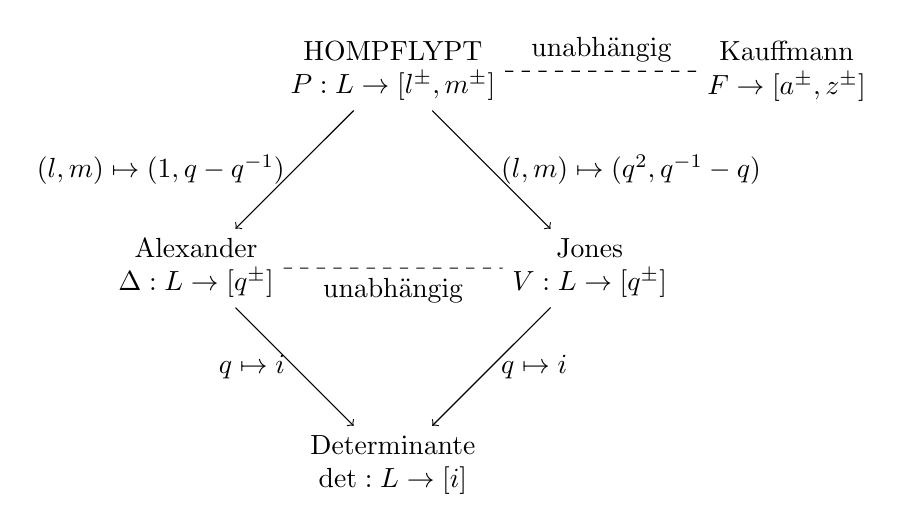
\begin{tikzpicture}[scale=2.5]
    \node[align=center] (1) at (1,2) {HOMPFLYPT \\ $P: \scr L \to \Z[l^\pm, m^\pm]$};
    \node[align=center] (2) at (0,1) {Alexander \\ $\Delta: \scr L \to \Z[q^\pm]$};
    \node[align=center] (3) at (2,1) {Jones \\ $V: \scr L \to \Z[q^\pm]$};
    \node[align=center] (4) at (1,0) {Determinante \\ $\det: \scr L \to \Z[i]$};
    \node[align=center] (5) at (3,2) {Kauffmann \\ $\scr F \to \Z[a^\pm, z^\pm]$};

    \draw[->] (1) -- node[left] {$(l,m) \mapsto (1, q - q^{-1})$} (2);
    \draw[->] (1) -- node[right] {$(l,m) \mapsto (q^2, q^{-1} - q)$} (3);
    \draw[->] (2) -- node[left] {$q \mapsto i$} (4);
    \draw[->] (3) -- node[right] {$q \mapsto i$} (4);
    \draw[dashed] (1) -- node[above] {unabhängig} (5);
    \draw[dashed] (2) -- node[below] {unabhängig} (3);
\end{tikzpicture}


% §E3
\section{Die Tait-Vermutung}

\begin{df}
    Ein Verschlingungs-Diagramm $D \subset \R^2$ heißt \emphdef{alternierend}, wenn beim Durchlaufen jeder Komponente abwechselnd Über/Unterkreuzungen auftauchen.

    Eine Verschlingung $L \subset \R^3$ heißt \emphdef{alternierend}, wenn sie sich durch ein alternierendes Diagramm darstellen lässt.
\end{df}

\begin{nt}
    \begin{itemize}
        \item
            In alternierenden Diagrammen ist kein R3-Zug möglich (die entsprechenden Situation können nicht auftreten):
        \item
            Ebensowenig ist ein reduzierender R2-Zug möglich (nicht-reduzierend möglich).
        \item
            Reduzierende R1-Züge sind möglich.
        \item
            Allgemeiner ist folgendes möglich: (zwei Teile, eins umkehren, „großer R1-Zug“ siehe Skizze)
    \end{itemize}
\end{nt}

\begin{df}
    Ein Diagramm heißt \emphdef{reduziert}, wenn keine solche Reduktion mehr möglich ist.
\end{df}

Die drei Tait-Vermutungen besagen
\begin{enumerate}[(1)]
    \item
        Jedes reduzierte, alternierende Verschlingungsdiagramm $D$ minimiert die Kreuzungsszahl, d.h. $D' \sim D \implies \Cr(D') \ge \Cr(D)$.
    \item
        Für reduzierte, alternierende Diagramme $D$ ist der Drall $w(D) = \sum_{p} \eps(p)$ eine Invariante, d.h. $D' \sim D$ mit $D, D'$ reduziert und alternierend impliziert $w(D) = w(D')$.
    \item
        Sind $D \sim D'$ reduzierte alternierende Diagramme, dann lassen sie sich allein durch Flypes (in $\S^2$) ineinander überführen.
\end{enumerate}
\begin{note}
    Klar ist $(3) \implies (2)$.
\end{note}
Dies löst das Klassifikationsproblem für alternierende Verschlingungen.


\begin{df}
    Jedes Polynom $P \in \Z[A^\pm]$, $P \neq 0$ schreibt sich eindeutig als
    \begin{math}
        P = \sum_{k=m}^n p_k A^k
    \end{math}
    mit $p_m \neq 0 \neq p_n$, $m \le n$.
    Wir setzen $\mindeg(P) := m$ und $\maxdeg(P) := n$ und $\width(P) := n - m$.
\end{df}

\begin{ex}
    \begin{enumerate}[1.]
        \item
            Beim Alexander-Polynom war $\width_q(\Delta(D) \le 4g(S_D)$.
            Gleichheit gilt falls $D$ zusammenhängend und alternierend ist (ohne Beweis).
        \item
            Wir wollen dies für Jones und die Kreuzungszahl $\Cr$ zeigen.
    \end{enumerate}
\end{ex}

\begin{df}
    Sei $D \subset \R^2$ ein unorientiertes Diagramm mit nummerierten Kreuzungen $i = 1, \dotsc, n$.
    Zu $s: \Set{1, \dotsc, n} \to \Set{\pm 1}$ definiere ein „aufgelöstes“ Diagramm $sD$ durch
    \begin{math}
        …
    \end{math}
    Sei $|sD|$ die Anzahl der Kreise und $\sum s := \sum_{i=1}^n s(i)$ die Summe der Vorzeichen.
\end{df}

\begin{lem}
    Für die Kaufmann-Klammer gilt
    \begin{math}
        \<D\> &= \sum_{s: \Set{1, \dotsc, n} \to \Set{\pm 1}} A^{\sum s} (-A^2 - A^{-2})^{|sD|-1} \\
        &=: \sum_{s} \< D | s\>
    \end{math}
\end{lem}

Ziel: Für reduzierte alternierende Diagramme wollen wir $\width(\<D\>)$ berechnen, genauer: höchste und niedrigste Terme verstehen.


\Timestamp{2015-07-13}

Definition: Distante Vereinigung.

\begin{df}
    Ein Diagramm $D$ heißt \emphdef{zusammenhängend}, wenn es nicht distante Vereinigung ist, d.h. $D = D_1 \sqcup D_2$ folgt entweder $D_1 = \emptyset$ oder $D_2 = \emptyset$.

    Ausführlich: Sei $S^1 \homto \C \subset \R^2$ eine (polygonale) Jordan-Kuve und $\R^2 \setminus C = A \sqcup B$ zwei Gebiete.
    Wenn $C \cap D = \emptyset$, dann entweder $A \cap D = \emptyset$ oder $B \cup D = \emptyset$.
\end{df}

Definition: Verbunde Summe von Diagrammen $D = D_1 \# D_2$.

\begin{df}
    Ein Diagramm $D$ heißt \emphdef{prim}, wenn es nicht verbundene Summe ist, d.h. aus $D = D_1 \# D_2$ folgt entweder $D_1$ oder $D_2$ trivial (ohne Kreuzungen).

    Ausführlich: Besteht $C \cap D$ aus zwei transversalen Schnittpunkten, dann ist entweder $A \cap D$ oder $B \cap D$ trivial, d.h. ein Bogen ohne Kreuzungen.
\end{df}

Dies sind Eigenschaften des Diagramms, nicht der zugrundeliegenden Verschlingung (Beispiele: zwei Kreiskompenten übereinander, nebeneinander und zwei Kleeblattschlingen als verbundene Summe nebeneneinander und teilweise übereinander).

\begin{st}
    Sei $D \subset \R^2$ ein unorientiertes Diagramm.
    Durch Auflösen einer Kreuzung erhalten wir aus $D$ die Diagramme $D_-$ oder $D_+$ (je nachdem wie die Kreuzung aufgelöst wurde).
    \begin{enumerate}[a)]
        \item
            Ist $D$ zusammenhängend, so auch $D_+$ oder $D_-$ (oder beide).
        \item
            Ist $D$ prim, so auch $D_+$ oder $D_-$ (oder beide).
    \end{enumerate}
    \begin{proof}
        \begin{enumerate}[a)]
            \item
                Angenommen $D$ ist zusammenhängend, aber weder $D_+$ noch $D_-$.
                Die trennenden Jordankurven $C_+, C_-$ müssen durch die aufgelösten Kreuzungen gehen (nach geeignetem Umformen nur einmal).
                Der Rand des Innenbereichs von $C_+$ und $C_-$ schneidet $D$ genau ein Mal, ein Widerspruch.
            \item
                Angenommen $D$ ist prim, aber weder $D_+$ noch $D_-$.
                Im Gegensatz zu oben sind hier jeweils zwei Fälle für $C_+$ und $C_-$ zu unterscheiden (Schnitte außen oder innen).
                Beim Schneiden von $C_+$ und $C_-$ sind weitere Fälle zu unterscheiden.
                $C_+ \cup C_-$ zerlegt die Ebene in vier offene Mengen (mit jeweils evtl. mehreren Zusammenhangskomponenten)
                \begin{math}
                    AA &= \Set{z \in \R^2 & \deg(C_-,z) = 0, \deg(C_+,z) = 0} \\
                    AB &= \Set{z \in \R^2 & \deg(C_-,z) = 0, \deg(C_+,z) = 1} \\
                    BA &= \Set{z \in \R^2 & \deg(C_-,z) = 1, \deg(C_+,z) = 0} \\
                    BB &= \Set{z \in \R^2 & \deg(C_-,z) = 1, \deg(C_+,z) = 1}.
                \end{math}
                Aus Paritätsgründen haben genau zwei dieser Bereiche $E_1, E_2$ genau zwei Schnitte mit $D$.
                Diese zwei Bereiche können nicht $AA$ und $BB$ sein.
                $D$ muss ohne Einschrankung in $E_1$ Kreuzungen enthalten ($C_+, C_-$ waren nicht-triviale Zerlegungen von $D_+, D_-$).
                $E_1$ liefert dann eine nicht-triviale Zerlegung für $D$, ein Widerspruch.
        \end{enumerate}
    \end{proof}
\end{st}

Die erste Tait-Vermutung wird präzisiert und umfassend beantwortet durch den folgenden Satz.

\begin{st}
    Sei $D \subset \R^2$ ein zusammenhängendes Verschlingungsdiagramm und $L \subset \R^3$ die dargestellte Verschlingung mit Jones-Polynom $V(L) \in \Z[q^\pm]$.
    \begin{enumerate}[a)]
        \item
            Es gilt
            \begin{math}
                \width_t V(L) = \frac{1}{2} \width_q V(L) \le \Cr(D).
            \end{math}
        \item
            Gleichheit gilt, wenn $D$ reduziert alternierend ist oder verbundene Summe solcher Diagramme ist.
        \item
            In allen anderen Fällen ist die Ungleichung strikt.
    \end{enumerate}
\end{st}


\Timestamp{2015-07-15}

\begin{lem}[Umschalten von $+$ nach $-$]
    Seien $s, s': \Set{1, \dotsc, n} \to \Set{\pm 1}$ mit $s(i) = +1$, $s'(i) = - 1$ für ein $i$ und $s(j) = s'(j)$ für alle $j \neq i$.

    Dann gilt $\sum s' = \sum s - 2$ und $|s'D| = |sD| \pm 1$.
    \begin{proof}
        Löse eine Kreuzung auf, beide Möglichkeiten: $\pm$.
        Die Zahl der Komponenten verändert sich jeweils genau um Eins.
    \end{proof}
\end{lem}

Erinnerung: $s_+, s_-: \Set{1, \dotsc, n} \to \Set{\pm 1}$ sind konstant $+1$, bzw. $-1$.

\begin{df}
    Ein Verschlingungsdiagramm $D$ heißt
    \begin{enumerate}[1)]
        \item
            \emphdef{plus-adäquat}, wenn $|s_+ D| > |sD|$ für alle $s$ mit $\sum s = n - 2$,
        \item
            \emphdef{minus-adäquat}, wenn $|s_- D| > |sD|$ für alle $s$ mit $\sum s = 2 - n$,
        \item
            \emphdef{adäquat}, wenn es plus- und minus-adäquat ist.
    \end{enumerate}
    \begin{nt}
        1) bedeutet: keiner der Kreise in $s_+ D$ stößt an sich selbst.
        2) analog.
    \end{nt}
\end{df}

\begin{ex}
    Diagramm des Achterknotens: $n = 4$.
    $|s_+ D| = 3 = |s_- D|$.
\end{ex}

\begin{lem}
    Jedes reduzierte alternierende Diagramm ist adäquat.
    \begin{proof}
        Wir färben die Regionen von $D$ schwarz und weiß (Schachbrettfärbung).
        Dann berandet $s_\pm D$ die schwarzen/weißen Regionen.
        Begründung: Jede Region ist berandet von einem Bögen mit alternierenden Kreuzungen.
        Zudem ist $D$ reduziert, daher stößt nie ein Kreis an sich selbst.
        Denn ein Kreis stößt genau dann in $s_\pm D$ an sich selbst, wenn ein „großer R1-Zug“ in $D$ möglich ist.
    \end{proof}
\end{lem}

\begin{lem}[A]
    Für jedes Verschlingungsdiagramm $D$ gilt
    \begin{enumerate}[1)]
        \item
            \begin{enumerate}[a)]
                \item
                    $\maxdeg_A \<D\> \le \Cr(D) + 2 |s_+ D| - 2$
                \item
                    Gleichheit gilt, wenn $D$ plus-adäquat ist.
            \end{enumerate}
        \item
            \begin{enumerate}[a)]
                \item
                    $\maxdeg_A \<D\> \ge -\Cr(D) - 2 |s_+ D| + 2$
                \item
                    Gleichheit gilt, wenn $D$ minus-adäquat ist.
            \end{enumerate}
    \end{enumerate}
    Also
    \begin{math}
        \width_A \<D\>  \le 2 \Cr(D) + 2 |s_+ D| + 2|s_- D| - 4
    \end{math}
    mit Gleichheit, wenn $D$ adäquat ist.
    \begin{proof}
        Erinnerung: Es gilt $\<D\> = \sum_s \<D|s\>$ mit $\<D|s\> = A^{\sum s} (-A^{\pm 2} - A^{-2})^{|sD| - 1}$.
        \begin{enumerate}[1)]
            \item
                \begin{enumerate}[a)]
                    \item
                        Es gilt
                        \begin{math}
                            \maxdeg_A \<D\> = \Cr(D) + 2(|s_+ D| - 1).
                        \end{math}
                        Beim Umschalten einer Kreuzung $s \to s'$ von $s(i) = +1$ nach $s'(i) = -1$ gilt $\sum s' = \sum s - 2$ und $|s' D| = |sD| \pm 1$.
                        Also $\maxdeg_A \<D|s'\> \le \maxdeg_A \<D|s\>$.
                        Daher gilt $\maxdeg_A \<D|s\> \le \maxdeg_A \<D|s_+\>$ für alle $s$.
                    \item
                        Wenn $D$ plus-adäquat ist, dann gilt bei jedem ersten Umschalten $s_+ \to s$ stets $|sD| = |s_+D| - 1$, also $\maxdeg_A \<D|s\> < \maxdeg_A \<D|s_+\>$.
                        Diese strikte Ungleichung gilt also für alle $s$.
                        Es kann also durch die Summation im höchsten Grad keine Auslöschung passieren, die Gleichheit wird angenommen.
                \end{enumerate}
            \item
                Analog
        \end{enumerate}
    \end{proof}
\end{lem}

\begin{lem}[B]
    \begin{enumerate}[a)]
        \item
            Ist $D$ zusammenhängend, dann gilt
            \begin{math}
                |s_+ D| + |s_- D| \le \Cr(D) + 2.
            \end{math}
        \item
            Gleichheit gilt, wenn $D$ alternierend ist oder verbundene Summe von alternierenden Diagrammen.
        \item
            In allen anderen Fällen ist die Ungleichung strikt.
    \end{enumerate}
    \begin{proof}
        \begin{enumerate}[a)]
            \item
                Induktion über $n = \Cr(D)$.
                Für $n = 0$ ist $D$ genau ein Kreis, $|s_+ D| = |s_- D| = 1$ und die Behauptung gilt.
                Sei nun $n \ge 1$.
                Da $D$ zusammenhängend ist, ist auch $D_+$ oder $D_-$ zusammenhängend.
                Sei nun $D_+$ ist zusammenhängend ($D_-$ analog).
                Dann ist $|s_+ D| = |s_+ D_+|$ und $|s_- D| = |s_- D_+| \pm 1$.
                Also
                \begin{math}
                    |s_+ D| + |s_- D|
                    &= |s_+ D_+| + |s_- D_+| \pm 1 \\
                    &\le (n-1) + 2 \pm 1 \\
                    &\le n + 2.
                \end{math}
            \item
                Wir betrachten die Schachbrettfärbung.
                Sei $D$ alternierend.
                $|s_+ D|$ sei die Anzahl der schwarzen Regionen und $|s_- D|$ die Anzahl der weißen Regionen.
                $r := |s_+ D| + |s_- D|$ die Anzahl aller Regionen.
                $D$ hat $n$ Kreuzungen und $k$ Kanten zwischen diesen.
                %Dann gilt für die Anzahl der Regionen
                %\begin{math}
                %    r := |s_+ D| + |s_- D|
                %\end{math}
                Es gilt $2k = 4n$, d.h. $k = 2n$.
                Für die Euler-Charakteristik gilt $\chi = n - k + r = 2$.
                Also
                \begin{math}
                    r = 2 - n + k
                    = 2 + n.
                \end{math}
                Die Gleichheit bleibt erhalten bei verbundener Summe:
                $|s_\pm D| = |s_\pm D_1| + |s_\pm D_2| - 1$.
                \begin{math}
                    |s_+ D| + |s_- D|
                    &= |s_+ D_1| + |s_- D_1| + |s_+ D_2| + |s_- D_2| - 2 \\
                    &= \Cr(D_1) + 2 + \Cr(D_2) + 2 - 2 \\
                    &= \Cr(D) + 2
                \end{math}
            \item
                Zeige: wenn $D$ prim, zusammenhängend, aber nicht alternierend, dann gilt strikte Ungleichung.
                Induktion: für $n = 0$ ist $D$ ein Kreis, also alternierend und nicht prim.
                Für $n = 1$ ist $D$ alternierend und prim, es gilt
                \begin{math}
                    |s_+ D| + |s_- D| = 3 = \Cr(D) + 2.
                \end{math}
                Für $n = 2$ ist das einzige nicht alternierende, prime Knotendiagramm zwei überlappende Kreise und
                \begin{math}
                    |s_+ D| + |s_- D| = 1 + 1 < \Cr(D) + 2 = 2 + 2.
                \end{math}
                Sei nun $n \ge 3$, dann existieren zwei aufeinanderfolgende nicht-alternierende Kreuzungen $1, 2$ und eine weiter Kreuzung $n$ mit $n \ge 3$.
                Wir lösen die $n$-te Kreuzung in $D_-, D_+$ auf.
                $D_-, D_+$ sind weiterhin alternierend.
                $D_-$ oder $D_+$ sind prim.
                Sei $D_+$ prim ($D_-$ analog).
                Dann gilt
                \begin{math}
                    |s_+ D_+| + |s_- D_+|
                    \le \Cr(D_+) + 1.
                \end{math}
                Also
                \begin{math}
                    |s_+ D| + |s_- D|
                    = |s_+ D_+| + |s_- D_+| \pm 1
                    \le n + 1
                    < n + 2.
                \end{math}
        \end{enumerate}
    \end{proof}
\end{lem}

\begin{st}
    Für jedes zusammenhängende Verschlingungsdiagramm $D$ gilt
    \begin{math}
        \width_A \<D\>
        \stack{A}\le 2 \Cr(D) + 2 |s_+ D| + 2|s_- D| - 4
        \stack{B}\le 4 \Cr(D).
    \end{math}
    Gleichheit gilt, wenn $D$ zudem reduziert und alternierend ist oder verbundene Summe von solchen.
    In allen anderen Fällen ist die Ungleichung strikt.

    Entsprechend gilt für das Jones-Polynom:
    \begin{math}
        \width_t V(D)
        \le \Cr(D).
    \end{math}
\end{st}

\Timestamp{2015-07-20}

\begin{kor}
    Sei $L \subset \R^3$ eine alternierende Verschlingung, d.h. $L$ lässt sich durch ein alternierendes Diagramm $D$ darstellen.
    Wir können $D$ als reduziert annehmen.
    Dann gilt
    \begin{math}
        \Cr(D) = \Cr(L) := \min \Set{\Cr(D') & \text{$D'$ stellt $L$ dar} }.
    \end{math}
    Zudem ist jedes minimale Diagramm reduziert und alternierend oder verbundene Summe von solchen.
\end{kor}

\begin{ex}
    \begin{itemize}
        \item
            Die Kleeblattschlinge lässt sich minimal alternierend mit drei Kreuzungen darstellen.
        \item
            Achterknoten
        \item
            Torusknoten/Torusverschlingung
        \item
            Hopf-Verschlingung
        \item
            Minimale Diagramme können verbundene Summe von reduzierten alternierenden Diagrammen sein.
            Die verbundene Summe selbst muss nicht alternierend sein.
    \end{itemize}
\end{ex}


\subsection{Die zweite Tait-Vermutung}

Zur zweiten Tait-Vermutung:
Wenn $D \sim D'$ reduziert und alternierend, dann haben sie gleichen Drall $w(D) = w(D')$.

\begin{ex}
    \begin{itemize}
        \item
            Für die Kleeblattschlinge gilt $w(3_1^\pm) = \pm 3$, also $3_1^+ \neq 3_1^t$.

            Dies ist unser vierter Beweis der Chiralität von $3_1$.
        \item
            Für den Achterknoten ist $w(D) = 0$.
            Dies deckt sich damit, dass der Achterknoten nicht chiral ist.
    \end{itemize}
\end{ex}

\begin{df}
    Sei $D$ ein Verschlingungsdiagramm.
    Die $r$-fache Kabelung $D^r$ von $D$ ist definiert durch „Ver-$r$-fachung“ jedes Stranges.
\end{df}

\begin{lem}
    Sind $D$ und $E$ R2/R3-äquivalent, so auch $D^r$ und $E^r$.
    \begin{proof}
        Leicht einzusehen.
    \end{proof}
    \begin{note}
        Für R1-Züge gilt dies nicht.
    \end{note}
\end{lem}

\begin{lem}
    Zwei Knotendiagramme $D, E$ sind genau dann R2/R3-äquivalent, wenn $D, E$ R-äquivalent sind und zudem $w(D) = w(E)$.

    Zwei Verschlingungsdiagramme $D = (D_1, \dotsc, D_n)$, $E = (E_1, \dotsc, E_n)$ sind genau dann R2/R3-äquivalent, wenn $D, E$ R-äquivalent sind und zudem $w(D_i) = w(E_i)$ für $i = 1, \dotsc, n$.
    \begin{proof} % leicht
        Die erste Implikation ist klar.

        Sei nun $D, E$ R-äquivalent.
        Ersetze jeden R1-Zug durch folgenden Whitney-Trick (bilde zwei Kringel, entgegengesetzt orientierte Kreuzungen).
        Den überzähligen Kringel können wir ausschließlich mittels R2/R3-Zügen auf der Komponente beliebig verschieben.

        Wir finden so eine Folge von R2/R3-Zügen von $D$ nach $E'$, wobei $E'$ bestehend aus $E$ und extra Kringel.
        Es gilt $w(D_i) = w(E_i')$.
        Da wir $w(D_i) = w(E_i)$ voraussetzen gilt $w(E_i') = w(E_i)$, d.h. es gibt auf jeder Komponente $E_i'$ gleich viele positive extra Kringel, wie negative extra Kringel.
        Durch paarweises Gruppieren heben sich diese mit dem Whitney-Trick auf.
    \end{proof}
\end{lem}

\begin{lem}
    Ist $D$ plus/minus-ädequat, so auch $D^r$.
    \begin{proof}
        Es gilt $s_\pm (D^r) \sim (s_\pm D)^r$, siehe Skizze.
    \end{proof}
\end{lem}

\begin{nt}
    Wir hatten gesehen: Ist $D$ reduziert alternierend, so auch adäquat, die Umkehrung gilt nicht.

    Die Verkabelung reduzierter alternierender Diagramme ist nie alternierend (für $\Cr(D) > 0$ und $r \ge 2$).
    Die Verkabelung adäquater Diagramme sind jedoch adäquat.
\end{nt}

\begin{st}
    Seien $D \sim D'$ reduziert und alternierende Knotendiagramme.
    \begin{enumerate}[1.]
        \item
            $\Cr(D) = \Cr(D')$,
        \item
            $w(D) = w(D')$.
    \end{enumerate}
    \begin{proof}
        Sei ohne Einschränkung $w(D') \le w(D)$, also $w(D') + a = w(D)$ mit $a \ge 0$.
        Ersetze $D'$ durch $E$, indem $a$ positive Kringel hinzugefügt werden.
        Es gilt $\Cr(D) = n$, $\Cr(E) = n + a$, $w(E) = w(D') + a = w(D)$.
        $D \sim E$ und $w(D) = w(E)$ folgt $D \stack{R2/3}\sim E$.
        Somit ist auch $D^r \stack{R2/3}\sim E^r$ und daher $\<D^r\> = \<E^r\>$.

        $D, D'$ sind reduziert und alternierend, also $D, D'$ adäquat.
        $E$ ist plus-adäquat, denn in $s_+ E$ entstehen lediglich $a$ neue triviale Komponenten.
        Somit ist $D^r, E^r$ plus-adäquat für alle $r$.
        Daher gilt
        \begin{math}
            \maxdeg_A \<D^r\> &= \Cr(D^r) + 2 |s_+ D^r| - 2 \\
            &= n r^2 + 2 r |s_+ D| - 2 \\
            \maxdeg_A \<E^r\> &= \Cr(E^r) + 2 |s_+ E^r| - 2 \\
            &= (n + a) r^2 + 2 r |s_+ E| - 2
        \end{math}
        Koeffizientenvergleich liefert $n = n + a$, $|s_+ D| = |s_+ E|$, d.h. $a = 0$.
    \end{proof}
\end{st}

\chapter{Differentialformen}

\begin{df} \label{6.1}
    Sei $V$ ein endlich-dimensionaler reeller Vektorraum und für $q \in \N_0$ sei $\omega \in {V^*}^{\otimes q}$ eine \emphdef{$q$-Form}, d.h. eine multilineare Abbildung $V^k \to \R$, $(v_1, \dotsc, v_q) \mapsto \omega(v_1, \dotsc, v_q)$.

    $\omega$ heißt \emphdef{alternierend}, falls $\omega(v_1, \dotsc, v_q) = 0$ wenn zwei der Argumente $v_1, \dotsc, v_q$ gleich sind.
\end{df}

\begin{ex*}
    Die Determinanten von rellen $n\times n$-Matrizen ist eine alternierende $n$-Form auf den Spalten (Zeilen) einer Matrix, $\det: (\R^n)^n \to \R$.
\end{ex*}

\begin{lem} \label{6.2}
    Sei $\omega \in {V^*}^{\otimes q}$ eine alternierende $q$-Form.
    Dann gilt für $i,j \in \Set{1, \dotsc, q}$, $\lambda \in \R$
    \begin{enumerate}[(i)]
        \item
            Scherung:
            \begin{math}
                \omega(v_1, \dotsc, v_{i-1}, v_i + \lambda v_j, v_{i+1}, \dotsc, v_q) = \omega(v_1, \dotsc, v_q)
            \end{math}
        \item
            Antikommutativität:
            \begin{math}
                \omega(v_1, \dotsc, v_j, \dotsc, v_i, \dotsc, v_q) = - \omega(v_1, \dotsc, v_i, \dotsc, v_j, \dotsc, v_q)
            \end{math}
        \item
            sind $v_1, \dotsc, v_q$ linear abhängig, dann gilt $\omega(v_1, \dotsc, v_q) = 0$.
    \end{enumerate}
    \begin{proof}
        leichte Übung (Linearität und alternierend).
    \end{proof}
\end{lem}


\chapter{Ramsey}

\Timestamp{2016-01-25}


\begin{st}
    Sei $G = (V,E)$ ein unendlicher Graph, d.h. $|V| = \infty$.
    Dann existiert ein unendlicher induzierter Untergraph $V'$, sodass $V'$ Clique oder unabhängig ist
    \begin{math}
        \alpha(G) + \omega(G) = \infty.
    \end{math}
    Allgemeiner:
    Sei $G$ vollständig und $f: \binom{V}{2} \to \Set{0, \dotsc, c - 1}$ eine Färbung in $c$ Farben.
    Dann existiert ein monochromatischer unendlicher Untergraph.
    \begin{proof}
        Sei ohne Einschränkung $V = \N$.

        Wähle für den Knoten $i = 1$ eine Farbe $g(i)$, sodass für fast alle $j > i$ gilt $f(\Set{i,j}) = g(i)$, eliminiere die restlichen Knoten.
        Wiederhole für $i = 2, 3, \dotsc$ mit den jeweils verbleibenden Knoten.

        Unter den verbleibenden (unendlich vielen) Knoten wähle eine Farbe mit unendlich vielen zugehörigen Knoten.
        Diese bilden eine Clique.
    \end{proof}
\end{st}

\begin{df}
    Ein \emphdef{Hypergraph} $G = (V, E)$ besteht aus einer Menge $V$ von \emphdef{Knoten} und einer Menge $E \subset \binom{V}{k}$ von \emphdef{Hyperkanten} für ein $k \in \N$.

    Sei $C = \Set{0, \dotsc, c-1}$ eine Menge von $c$ Farben.
    Eine Färbung des vollständigen Hypergraphen $(V, \binom{V}{k})$ ist eine Abbildung $f: \binom{V}{k} \to C$.

    Eine Teilmenge $V' \subset V$ heißt \emphdef{monochromatisch}, falls $f(K) \in C$ konstant ist für alle $K \in \binom{V'}{k}$.
\end{df}

\begin{st}[Ramsey, 1930]
    Für alle $n, k, c \in \N$ existiert eine Zahl $R(n,k,c) \in \N$ minimal mit der folgenden Eigenschaft:
    % Für jeden Hypergraphen G = (V,E) mit $|V| \ge R(n,k,c)$ und jeder Färbung ...
    Ist $f: \binom{V}{k} \to \Set{0, \dotsc, c-1}$ eine Färbung für $|V| \ge R(n,k,c)$, dann existiert $V' \subset V$ mit $|V'| \ge n$ und $V'$ ist monochromatisch.
    \begin{proof}
        Induktionsanfang:
        \begin{math}
            R(n,1,c) = c(n-1) + 1.
        \end{math}
        Sei $r \in \N$ und $f: \binom{V}{k} \to C = \Set{0, \dotsc, c-1}$ mit $|V| \ge r$.
        Wir definieren induktiv Mengen $A_m, B_m \subset V$ mit den folgenden Eigenschaften:
        \begin{enumerate}[(i)]
            \item
                $\forall a \in A_m \forall b \in B_m: a < b$,
            \item
                $|A_m| = m$,
            \item
                Es gibt eine Färbung $g: \binom{A_m}{k-1} \to C$ mit der Eigenschaft, dass für alle $K \subset \binom{A_m}{k-1}$ gilt $f(K, b) = g(K)$ für alle $b \in B_m$.

                Für $K \in \binom{V}{k-1}$ und $b \in V$ mit $b > \max(K)$ bezeichne $K, b$ die Menge $K \cup \Set{b}$.
        \end{enumerate}
        Setze $A_0 :=  \emptyset$ und $B_0 := V$.

        Seien $A_m$ und $B_m$ bereits definiert.
        Wähle $a_{m+1} := \min B_m$ und setze $A_{m+1} = A_m \cup \Set{a_{m+1}}$.
        Wir wählen jetzt $B_{m+1} \subset B_m \setminus \Set{a_{m+1}}$ geeignet.

        Gesucht ist eine Erweiterung der Färbung zu $g: \binom{A_{m+1}}{k-1} \to C_m$ mit Eigenschaft (iii).
        $g(K)$ ist noch nicht definiert genau dann, wenn $a_{m+1} \in K$.
        Es müssen also noch insgesamt $\binom{m}{k-2}$ solcher $K$ gefärbt werden.

        Für $a_{m+1} \in K \in \binom{A_m}{k-1}$ wähle $s \in C$ mit $\Set{b \in B_m & f(K,b) = s}$ maximal.
        Dann färbe $g(K) = s$.

        Setze
        \begin{math}
            B_{m+1} = \Set{ b \in B_m \setminus \Set{a_{m+1}} & \forall a_{m+1} \in K \in \binom{A_{m+1}}{k-1} : f(K,b) = s_K }.
        \end{math}
        Dann gilt (i), (ii), (iii).

        Betrachte den Ausdünnungsprozess nacheinander für die $a_{m+1} \in K \in \binom{A_{m+1}}{k-1}$.
        Jedes Mal können wir $\frac{1}{|C|}$ Knoten weiter fortfahren.

        Wenn wir also $|B_{m+1}| \ge r$ garantieren wollen, müssen wir mit $|B_m| \ge c^{\binom{m}{k-2}} r$ starten.
        Für $R(n,k,c)$ müssen wir $A_m$ mit $|B_{m+1}| \ge 1$ erreichen mit $m = n - 1$.
        Also ist
        \begin{math}
            R(n,k,c) \le \prod_{m < R(n,k-1,c)} c^{\binom{m}{k-2}}
            = c^{\sum_{m < R(n,k-1,c)} \binom{m}{k-2}}
            = c^{\binom{R(n,k-1,c)}{k-1}}
        \end{math}
    \end{proof}
\end{st}

\begin{ex}
    $R(n) := R(n, 2, 2)$ ist die Situation für Graphen $(V, E)$.
    \begin{itemize}
        \item
            $R(1) = 0$
        \item
            $R(2) = 2$,
        \item
            $R(3) = 6$,
            denn $R(3) \neq 5$ wegen
            $\alpha(C_5) = 2 = \omega(C_5)$
    \end{itemize}
\end{ex}

\chapter{Einführung in die algebraische Zahlentheorie}


\begin{df} \label{8.1}
	Sei $L / K$ eine endliche Körpererweiterung, $x \in L$.

	Wir bezeichnen mit $T_x: L \to L$ den $K$-linearen Endomorphismus $a \mapsto x a$, die Linksmultiplikation mit $x$.
	\begin{enumerate}[a)]
		\item
			Die Spur von $T_x$ nennt man die \emphdef{Spur} $\Tr_{L/K}(x)$.
		\item
			Die Determiante von $T_x$ nennt man die \emphdef{Norm} $N_{L/K}(x)$.
	\end{enumerate}
\end{df}

% Bsp + Bem
\begin{nt} \label{8.2}
	\begin{enumerate}[a)]
		\item
			Spur und Determinante von Vektorraumendomorphismen sind unabhängig von der Wahl der Basis.
		\item
			Ist
			\[
				\chi_{T_x}(t)
				= t^n - a_1 t^{n-1} + \dotsb + (-1)^n a_n
			\]
			mit $a_1 \in K$ das charakteristische Polynom von $T_x$, dann ist $\Tr_{L/K}(x) = a_1$ und $N_{L/K}(x) = a_n$.

			Ist $M_x = (m_{ij})$ die zu $T_x$ gehörige Matrix in einer Matrixdarstellung nach Wahl einer Basis, dann ist $\Tr_{L/K}(x) = \sum_{i=1}^n m_{ij}$, $n = \dim_K L$ und $N_{L/K}(x) = \det M_x$.
		\item
			Sei $L = \Q(\sqrt d)$ mit $d \in \Z$ quadratfrei.
			Wähle $\Set{1, \sqrt d}$ als $\Q$-Basis.
			Setze $x = a + b \sqrt d$ mit $a, b \in \Q$.
			Dann ist $M_x = \Matrix{a & bd \\ b & a}$ wegen $x \sqrt d = a \sqrt d + b d$.
			Also ist
			\begin{align*}
				\Tr_{L/\Q}(x) &= 2a, &
				N_{L/\Q}(x) &= a^2 - db^2.
			\end{align*}
	\end{enumerate}
\end{nt}

% Lem 8.3
\begin{lem} \label{8.3}
	\begin{enumerate}[a)]
		\item
			Die Abbildung $L \to K, x \mapsto \Tr_{L/K}(x)$ ist ein Gruppenhomomorphismus $(L, +) \to (K, +)$ und es gilt
			\[
				\Tr_{L/K}(kx) = k \Tr_{L/K}(x)
			\]
			für $k \in K$.
		\item
			Die Abbildung $L^* \to K^*, x \mapsto N_{L/K}(x)$ ist ein Gruppenhomomorphismus $(L^*, \cdot) \to (K^*, \cdot)$ zwischen den Einheitengruppen von $L$ und $K$.
	\end{enumerate}
	\begin{proof}
		Einfach nachzurechnen (Spur ist additiv, Determinante multiplikativ, \dots).
	\end{proof}
\end{lem}

% Wiederholung ... 8.4
\begin{nt}[Wiederholung von Begriffen und Sätzen aus der Algebra] \label{8.4}
	\begin{enumerate}[a)]
		\item
			Eine Körpererweiterung $L / K$ heißt \emphdef{separabel}, wenn jedes Element $x \in L$ ein Minimalpolynom $\mu_x \in K[x]$ besitzt, welches in einem algebraisch abgeschlossenen Körper $\_K$ keine mehrfachen Nullstellen hat.
		\item
			Körpererweiterungen über Körper der Charakteristik 0 sind separabel.
			Insbesondere ist $L / \Q$ mit algebraischem Zahlkörper $L$ stets separabel.
			Für algebraische Zahlkörper kann man $\_K = \C$ wählen.
		\item
			Sei $L / K$ separabel und $\dim_K L = n$.
			Dann gibt es genau $n$ verschiedene $K$-Homomorphismen $\sigma_i: L \to \_K$.
			Dabei ist ein $K$-Homomorphismus ein Körperhomomorphismus, der $K$ elementweise festlässt, d.h. $\sigma_i(k) = k$ für alle $k \in K$.
	\end{enumerate}
\end{nt}

% St 8.5
\begin{st} \label{8.5}
	Sei $L / K$ separabel, $n = \dim_K L$ und $\Hom_K(L, \_K) = \Set{\sigma_1, \dotsc, \sigma_n}$ die Menge der $K$-Homomorphismen nach $\_K$.
	Dann gilt für ein $x \in L$, dass
	\begin{enumerate}[(i)]
		\item
			$\chi_{T_x}(t) = \prod_{i=1}^n (t - \sigma_i(x))$,
		\item
			$\Tr_{L/K}(x) = \sum_{i=1}^n \sigma_i(x)$,
		\item
			$N_{L/K}(x) = \prod_{i=1}^n \sigma_i(x)$.
	\end{enumerate}
	\begin{proof}
		(ii) und (iii) folgen unmittelbar aus (i).
	\end{proof}
	\begin{note}
		Ist $L / K$ sogar galoissch, dann bilden $\Set{\sigma_1, \dotsc, \sigma_n}$ die Galoisgruppe und $\sigma_i$ sind insbesondere Körperautomorphismen von $L$.
	\end{note}
\end{st}


\printindex[lectures]
\printindex[terms]
%\printbibliography


\end{document}
